\chapter{Supplementary material from the analysis of invisibly decaying Higgs bosons}
\label{app:supplementary_hinv_plots}

\initial{T}o avoid detracting too much from the predominant results from Chpt.~\ref{chap:higgstoinv}, some figures were omitted from the main text. The following sections illustrate the pre-fit and post-fit distributions for the \glspl{CR} in each category and data taking period.


%=========================================================


\section{Post-fit distributions of the control regions in the \texorpdfstring{\ttH}{ttH} category}
\label{sec:pre_post_fit_plots_ttH_CRs}

\begin{figure}[htbp]
    \centering
    \begin{subfigure}[b]{0.66\textwidth}
        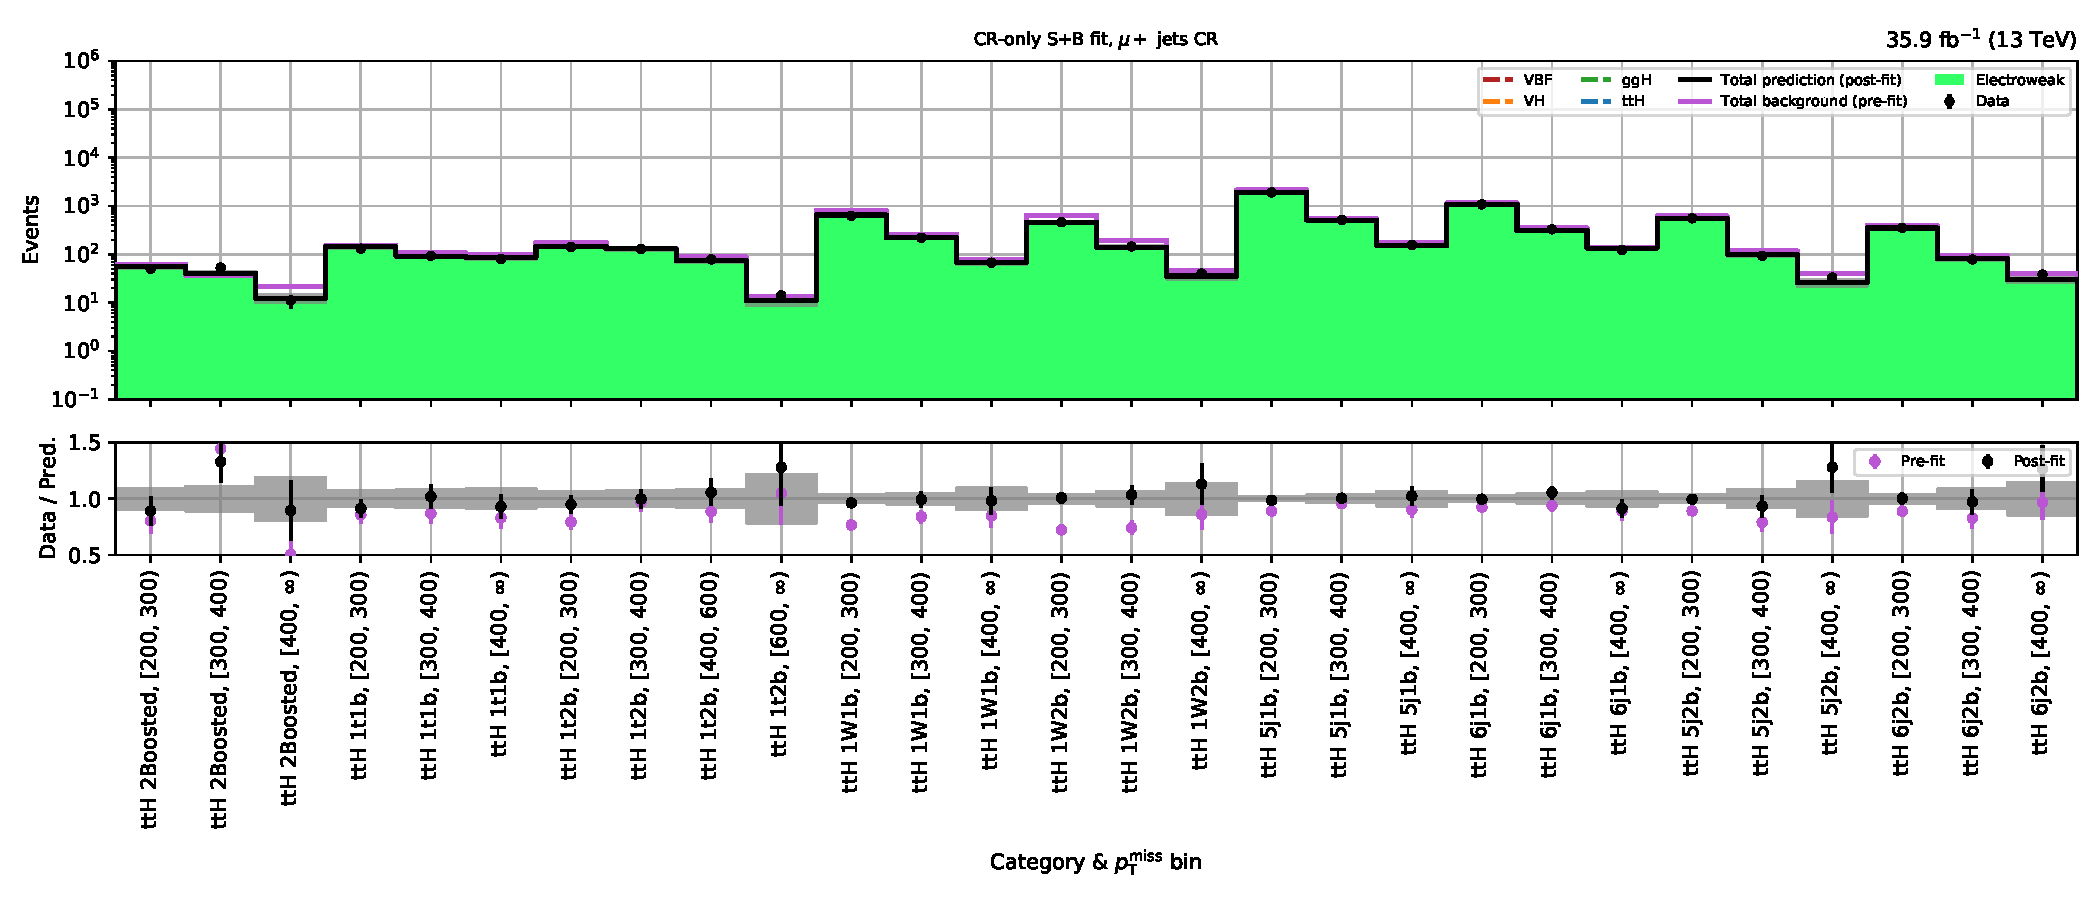
\includegraphics[width=\textwidth]{chapters/higgstoinv/figures/mountain_ranges/2016/ttH/Wmunu_tree_fit_s-abs_values_ttH_cats.pdf}
        \caption{\ttH --- \singleMuCr \gls{CR} (2016)}
    \end{subfigure}

    \begin{subfigure}[b]{0.66\textwidth}
        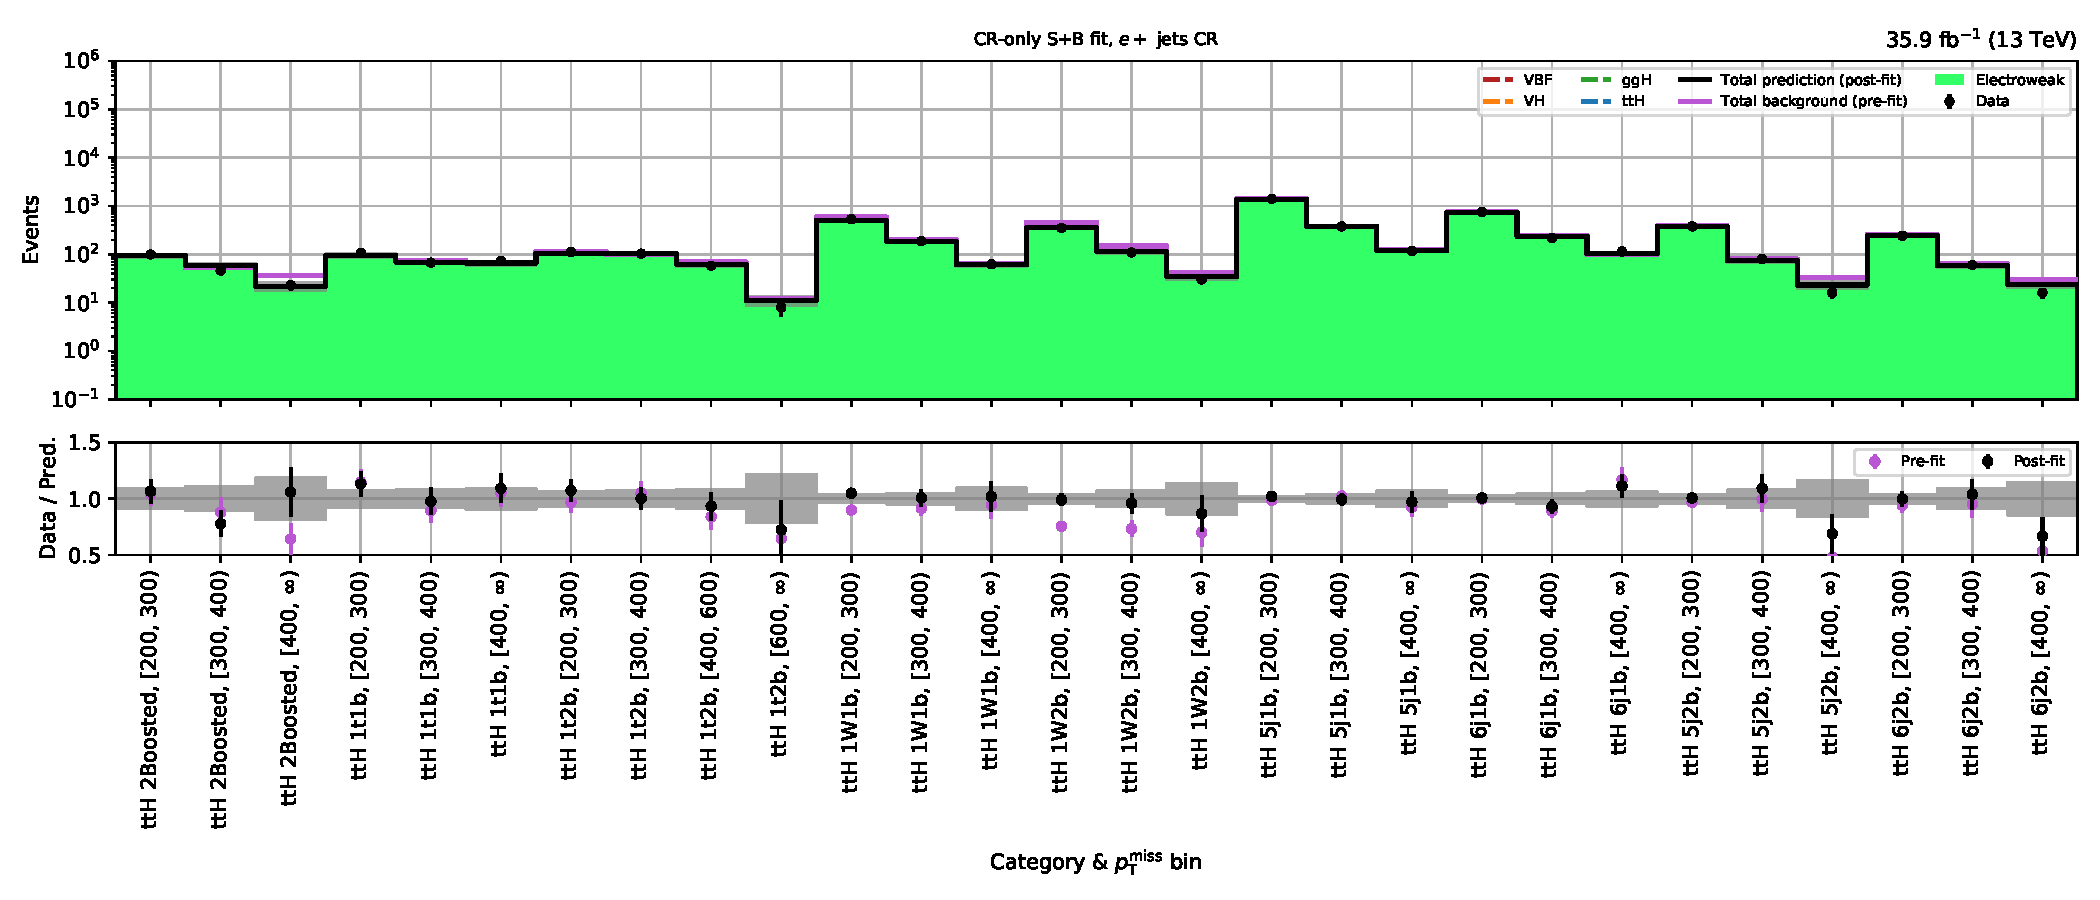
\includegraphics[width=\textwidth]{chapters/higgstoinv/figures/mountain_ranges/2016/ttH/Wenu_tree_fit_s-abs_values_ttH_cats.pdf}
        \caption{\ttH --- \singleEleCr \gls{CR} (2016)}
    \end{subfigure}

    \begin{subfigure}[b]{0.66\textwidth}
        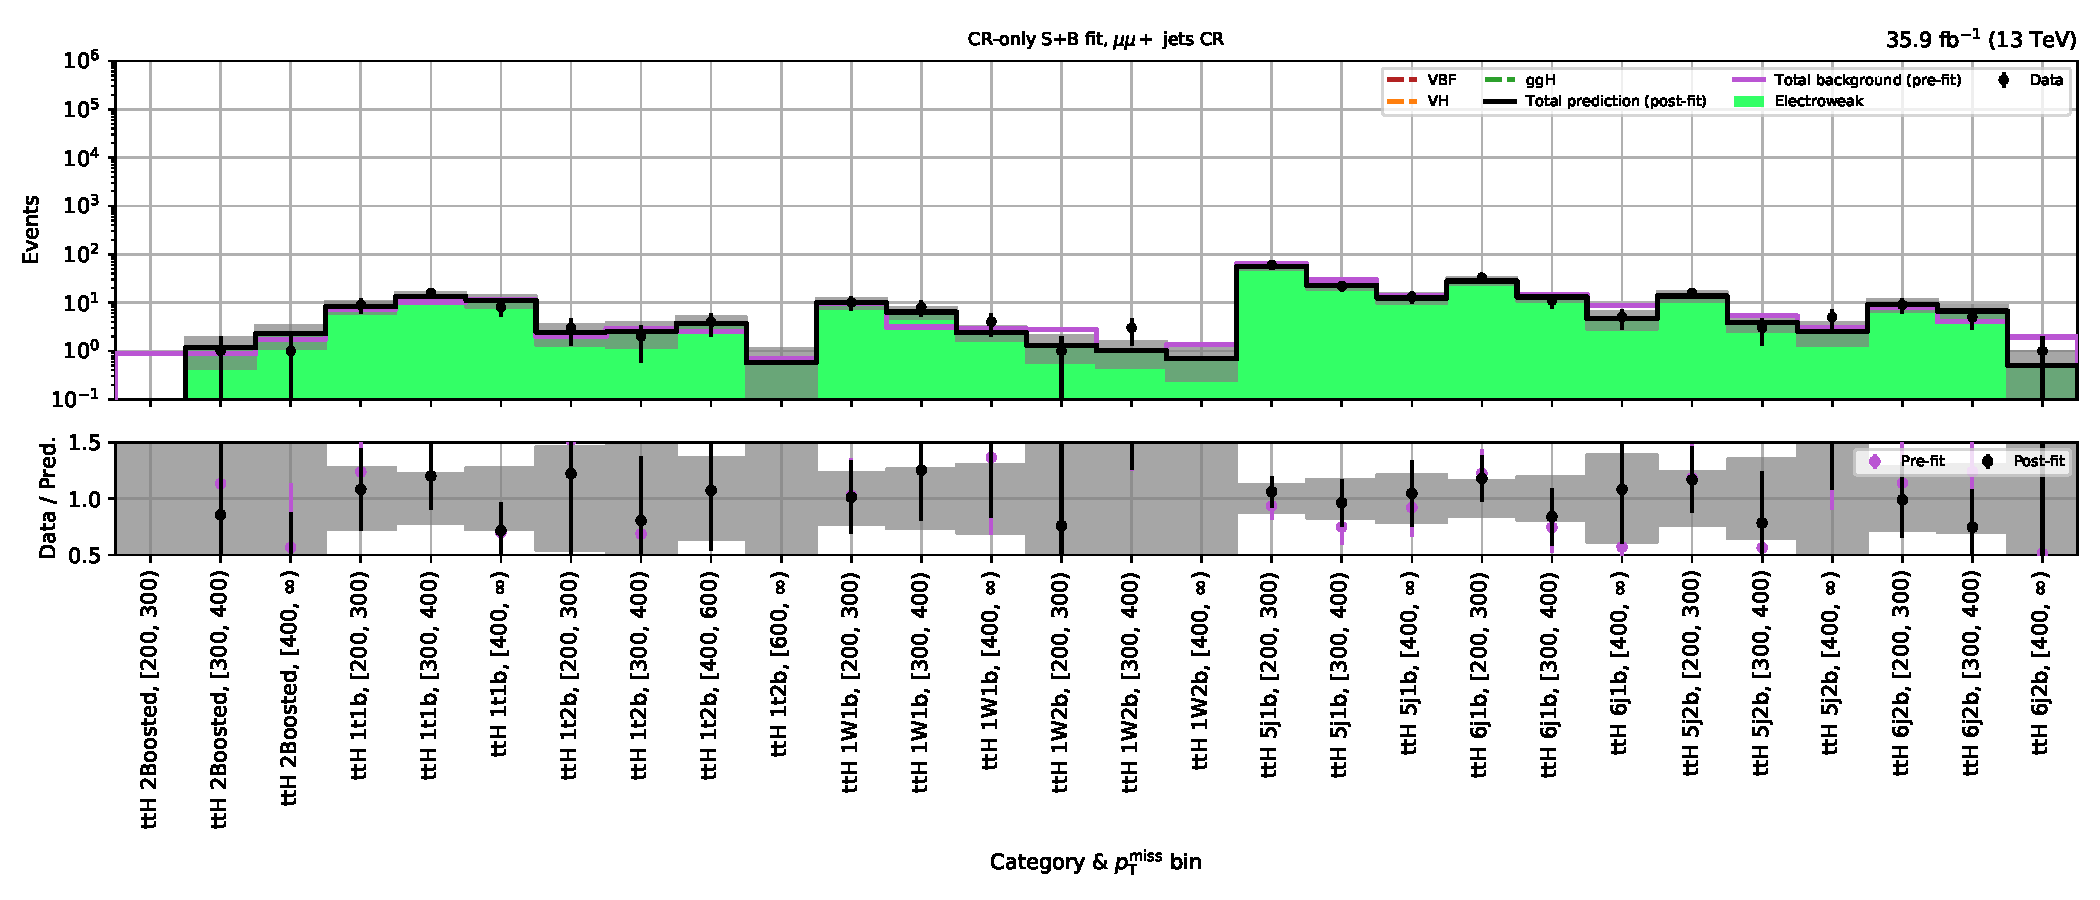
\includegraphics[width=\textwidth]{chapters/higgstoinv/figures/mountain_ranges/2016/ttH/Zmumu_tree_fit_s-abs_values_ttH_cats.pdf}
        \caption{\ttH --- \doubleMuCr \gls{CR} (2016)}
    \end{subfigure}

    \begin{subfigure}[b]{0.66\textwidth}
        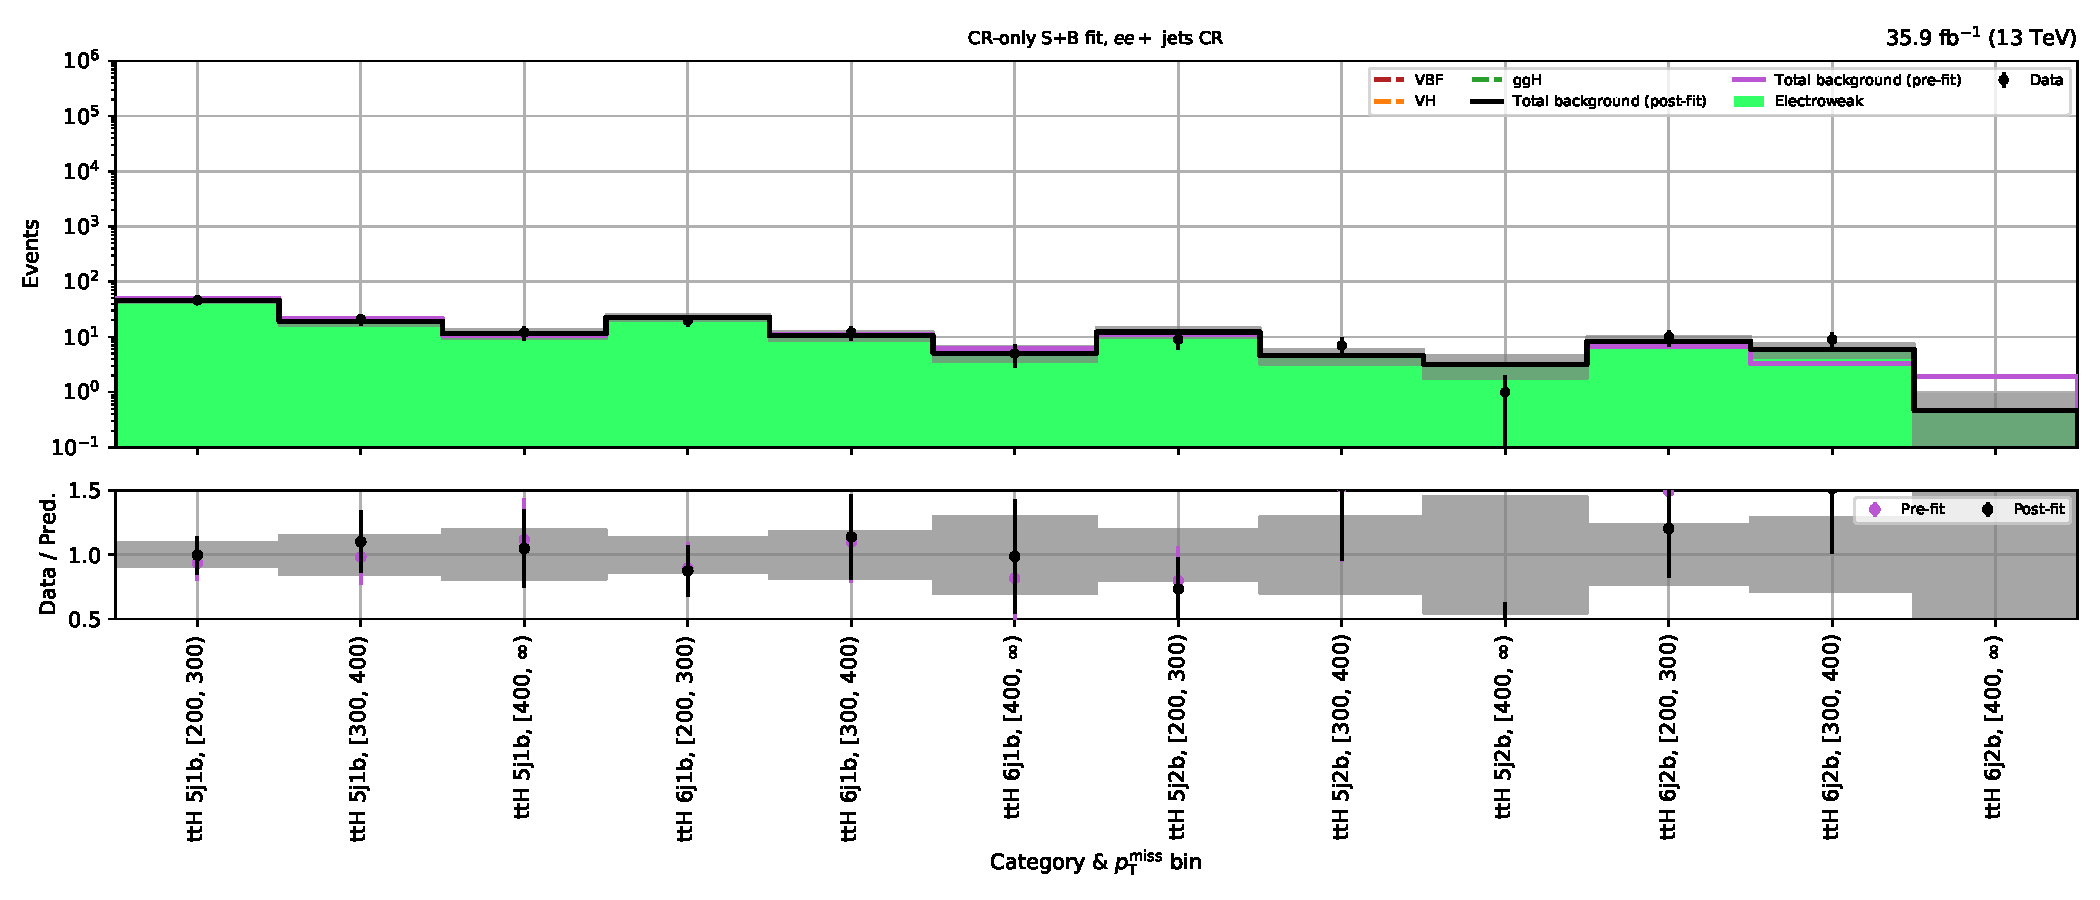
\includegraphics[width=\textwidth]{chapters/higgstoinv/figures/mountain_ranges/2016/ttH/Zee_tree_fit_s-abs_values_ttH_cats.pdf}
        \caption{\ttH --- \doubleEleCr \gls{CR} (2016)}
    \end{subfigure}
    \caption[Post-fit yields for each \ttH subcategory and \ptmiss bin in the lepton control regions for the 2016 dataset]{Post-fit yields for each \ttH subcategory and \ptmiss bin in the lepton \glspl{CR} for the 2016 dataset. The total background pre-fit and post-fit is compared in the lower panel of each subfigure.}
    \label{fig:htoinv_mountain_range_ttH_2016_CRs}
\end{figure}

\begin{figure}[htbp]
    \centering
    \begin{subfigure}[b]{0.66\textwidth}
        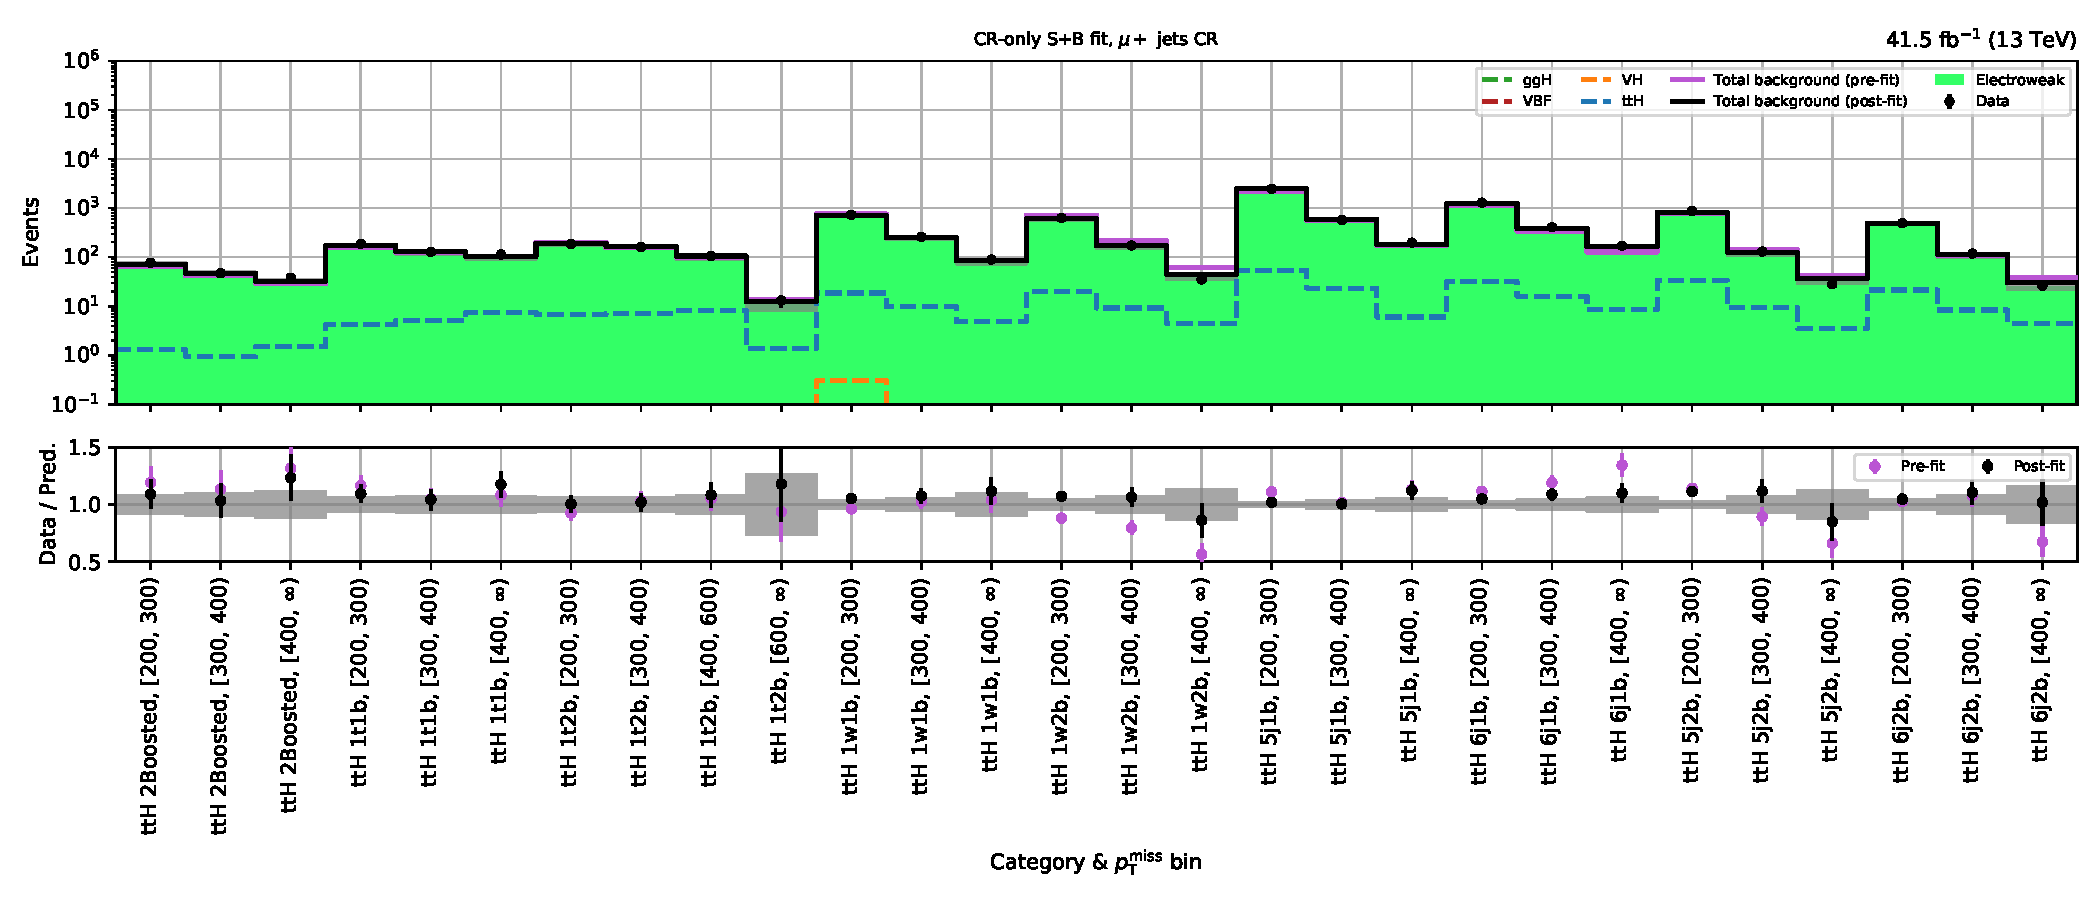
\includegraphics[width=\textwidth]{chapters/higgstoinv/figures/mountain_ranges/2017/ttH/Wmunu_tree_fit_s-abs_values_ttH_cats.pdf}
        \caption{\ttH --- \singleMuCr \gls{CR} (2017)}
    \end{subfigure}

    \begin{subfigure}[b]{0.66\textwidth}
        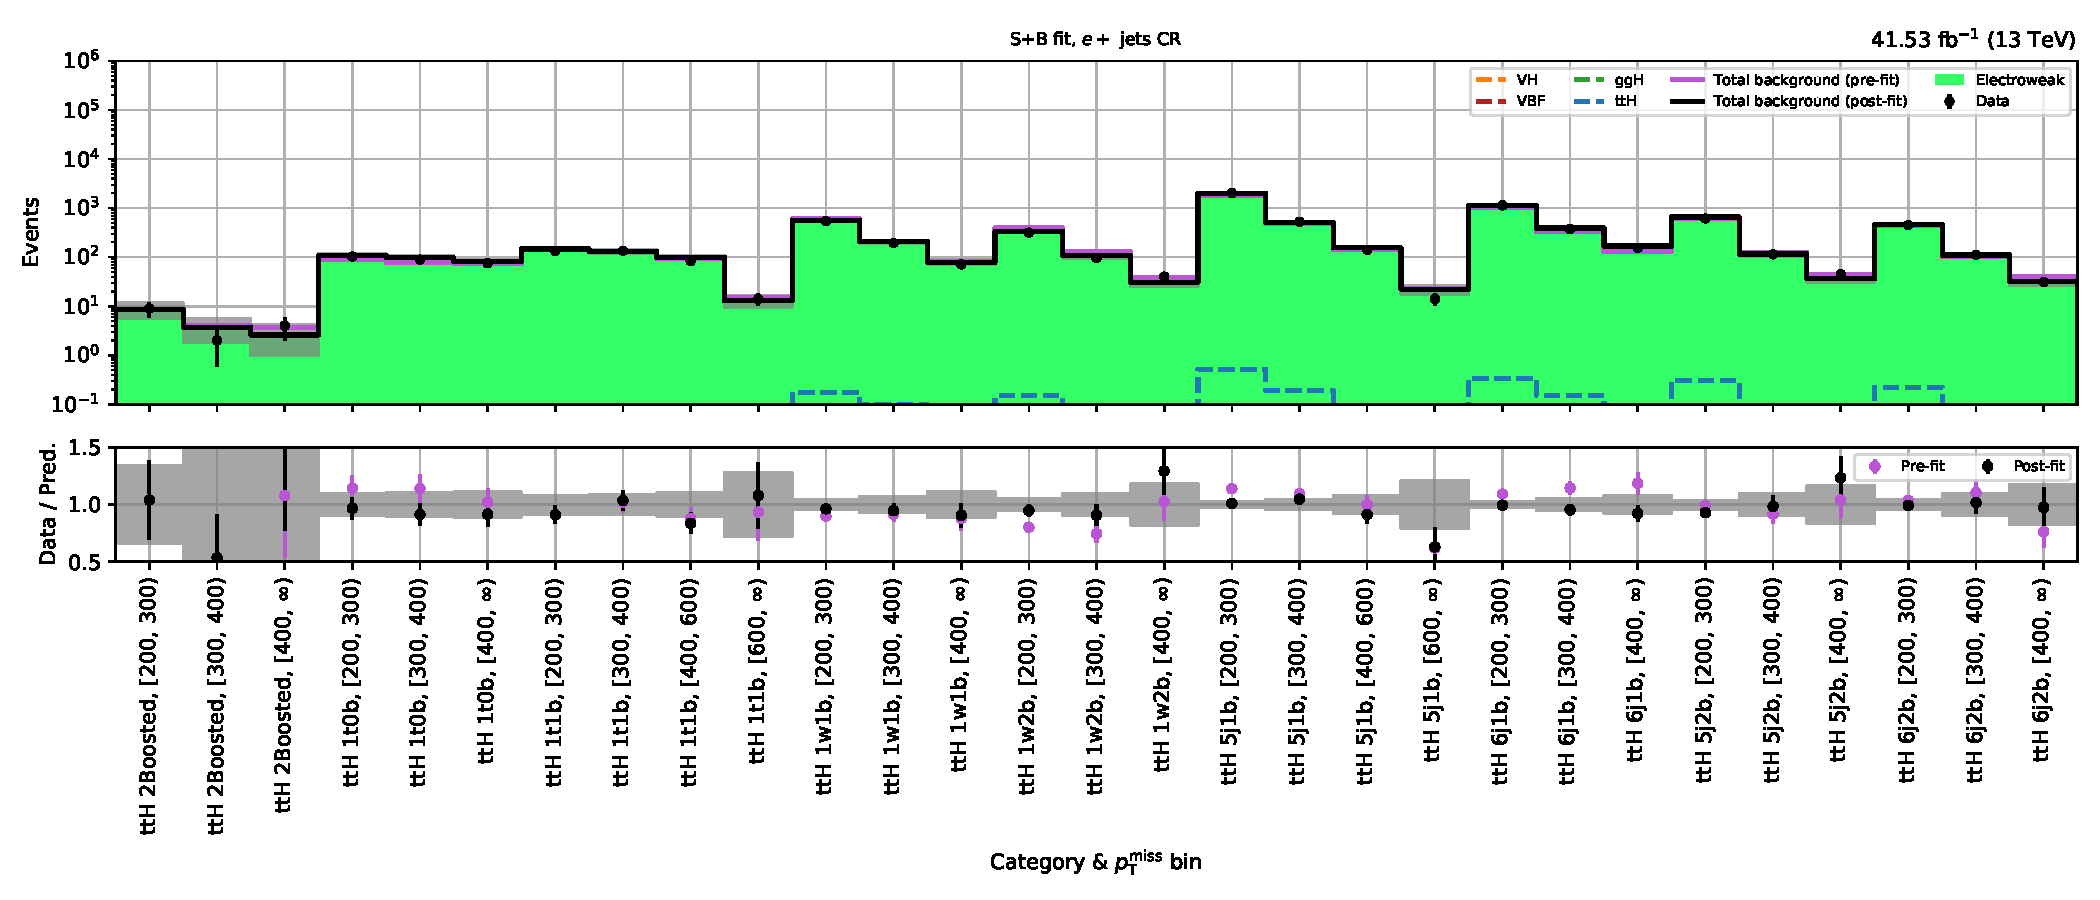
\includegraphics[width=\textwidth]{chapters/higgstoinv/figures/mountain_ranges/2017/ttH/Wenu_tree_fit_s-abs_values_ttH_cats.pdf}
        \caption{\ttH --- \singleEleCr \gls{CR} (2017)}
    \end{subfigure}

    \begin{subfigure}[b]{0.66\textwidth}
        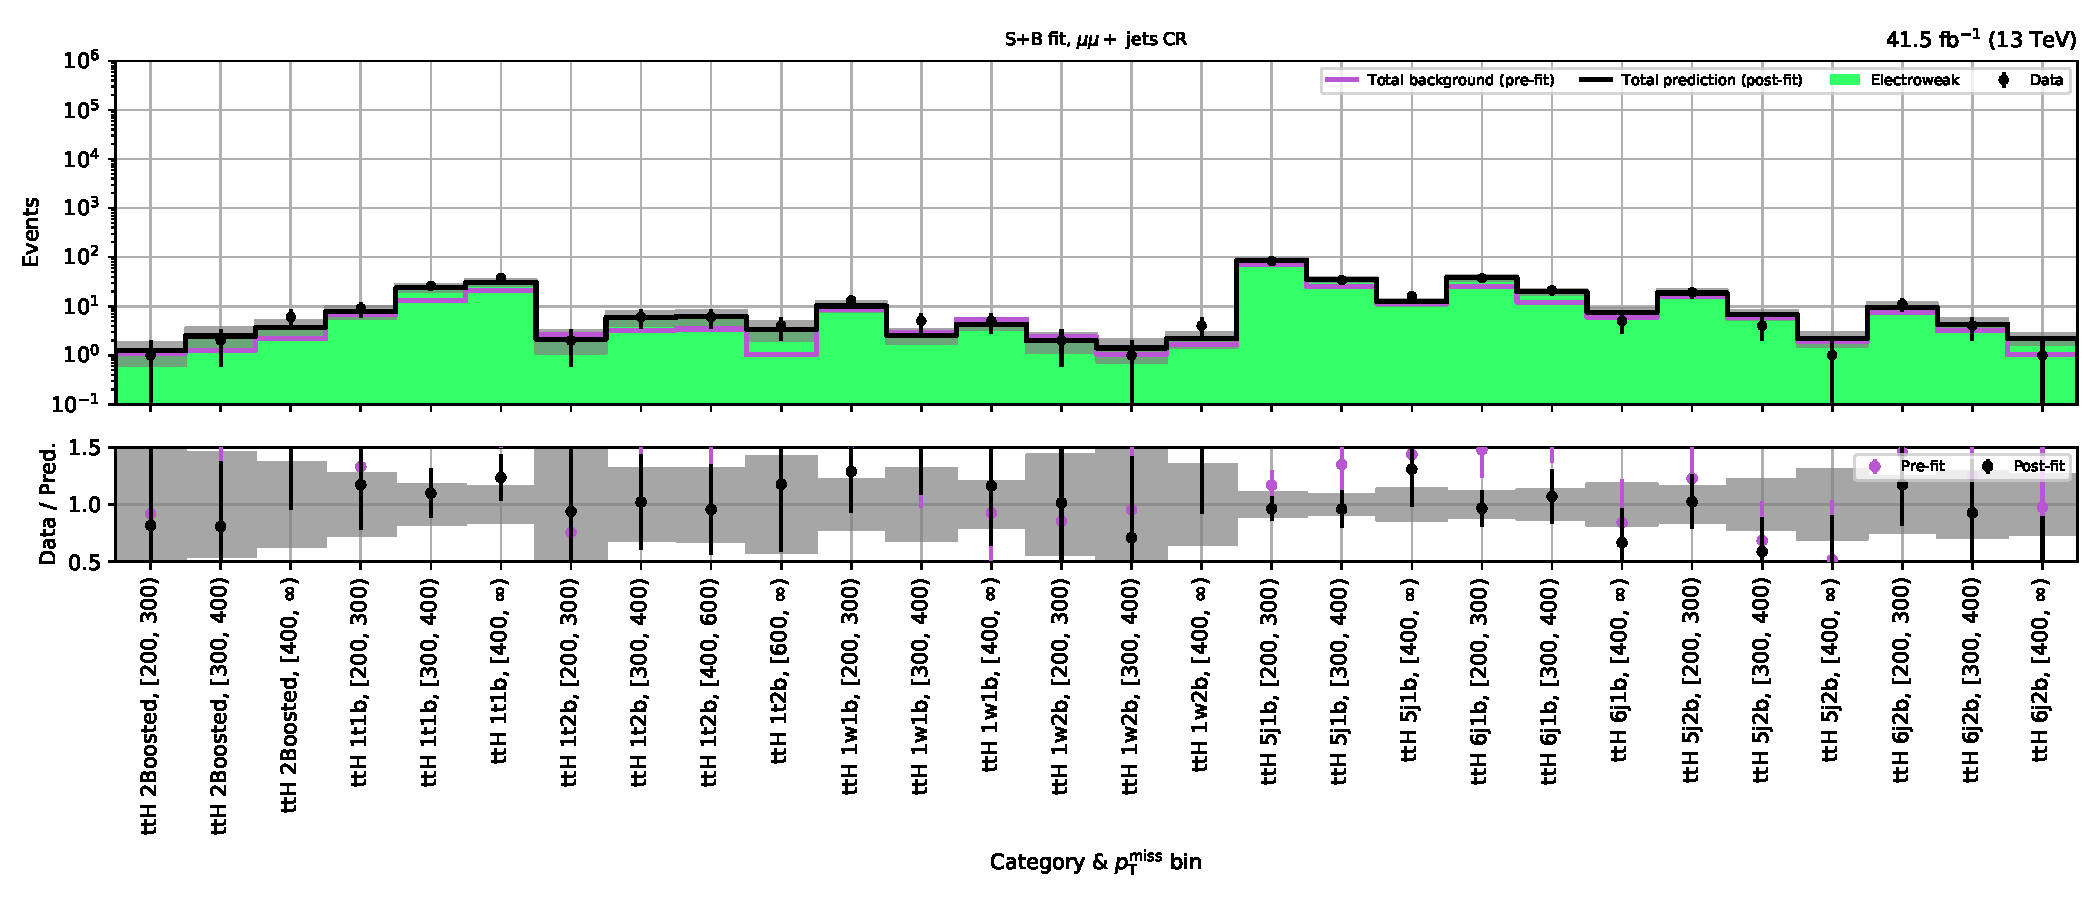
\includegraphics[width=\textwidth]{chapters/higgstoinv/figures/mountain_ranges/2017/ttH/Zmumu_tree_fit_s-abs_values_ttH_cats.pdf}
        \caption{\ttH --- \doubleMuCr \gls{CR} (2017)}
    \end{subfigure}

    \begin{subfigure}[b]{0.66\textwidth}
        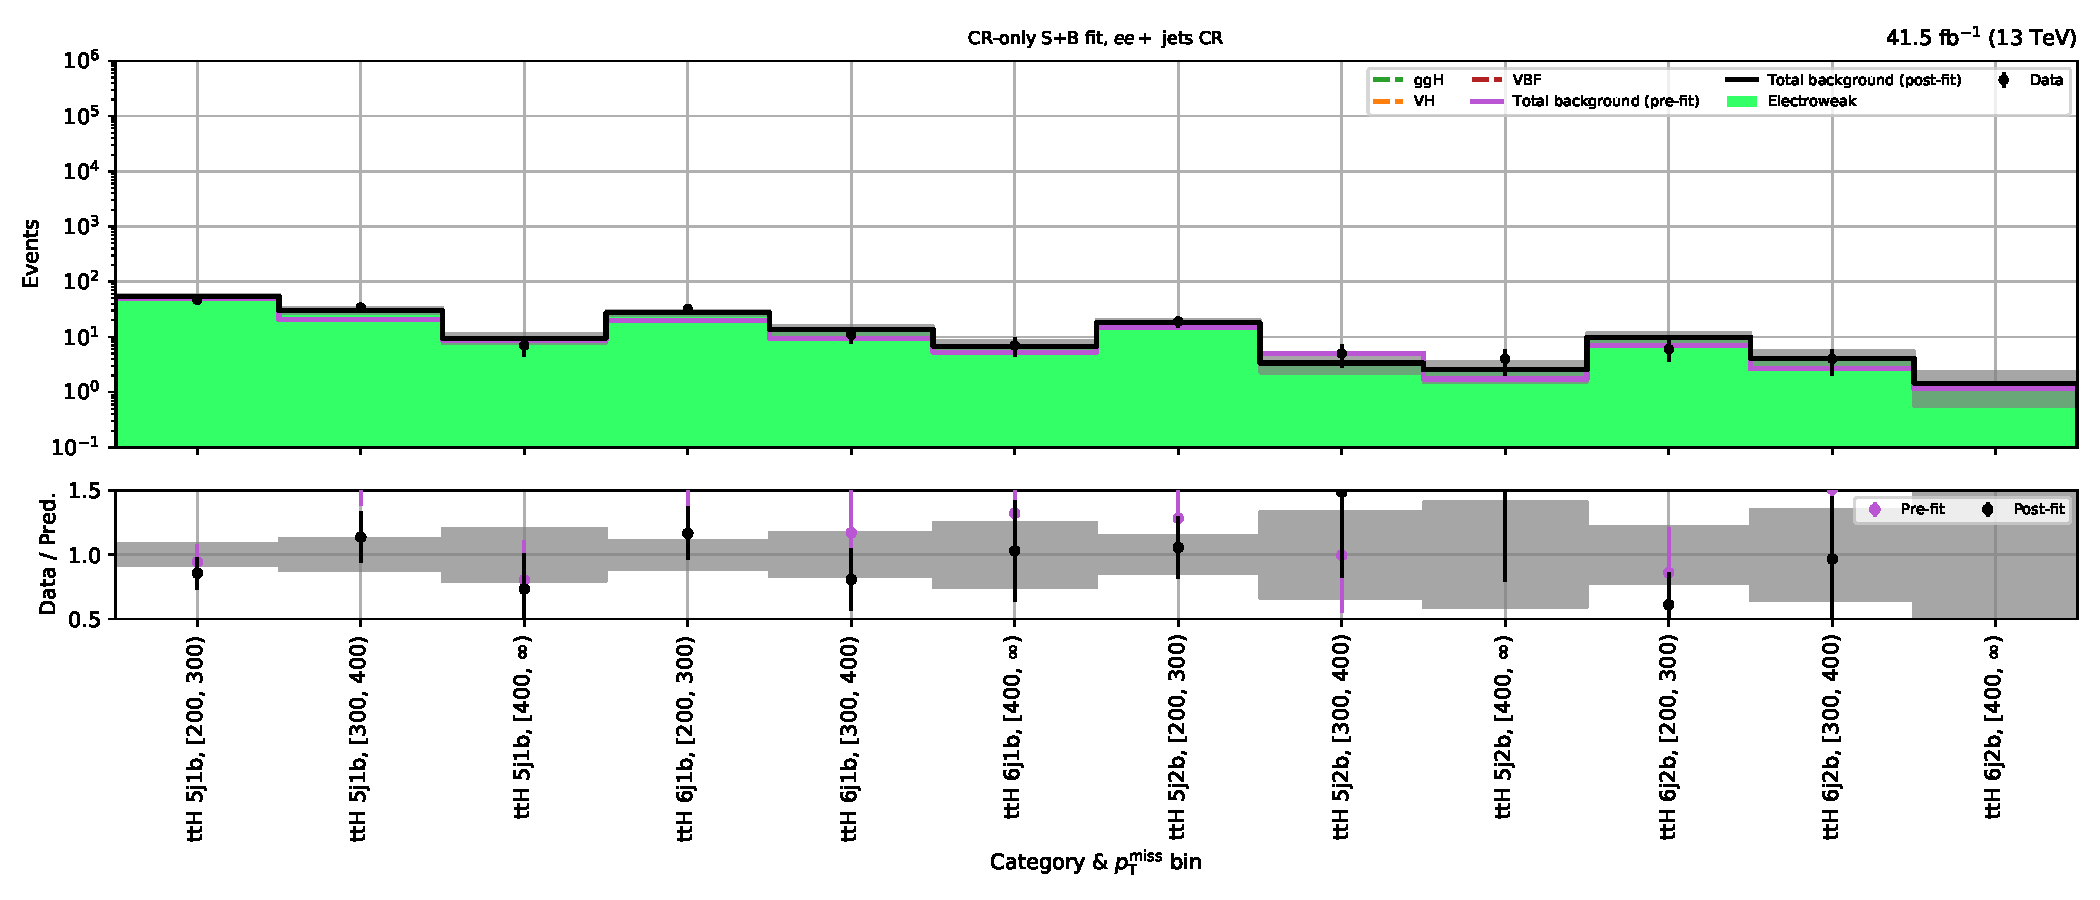
\includegraphics[width=\textwidth]{chapters/higgstoinv/figures/mountain_ranges/2017/ttH/Zee_tree_fit_s-abs_values_ttH_cats.pdf}
        \caption{\ttH --- \doubleEleCr \gls{CR} (2017)}
    \end{subfigure}
    \caption[Post-fit yields for each \ttH subcategory and \ptmiss bin in the lepton control regions for the 2017 dataset]{Post-fit yields for each \ttH subcategory and \ptmiss bin in the lepton \glspl{CR} for the 2017 dataset. The total background pre-fit and post-fit is compared in the lower panel of each subfigure.}
    \label{fig:htoinv_mountain_range_ttH_2017_CRs}
\end{figure}

\begin{figure}[htbp]
    \centering
    \begin{subfigure}[b]{0.66\textwidth}
        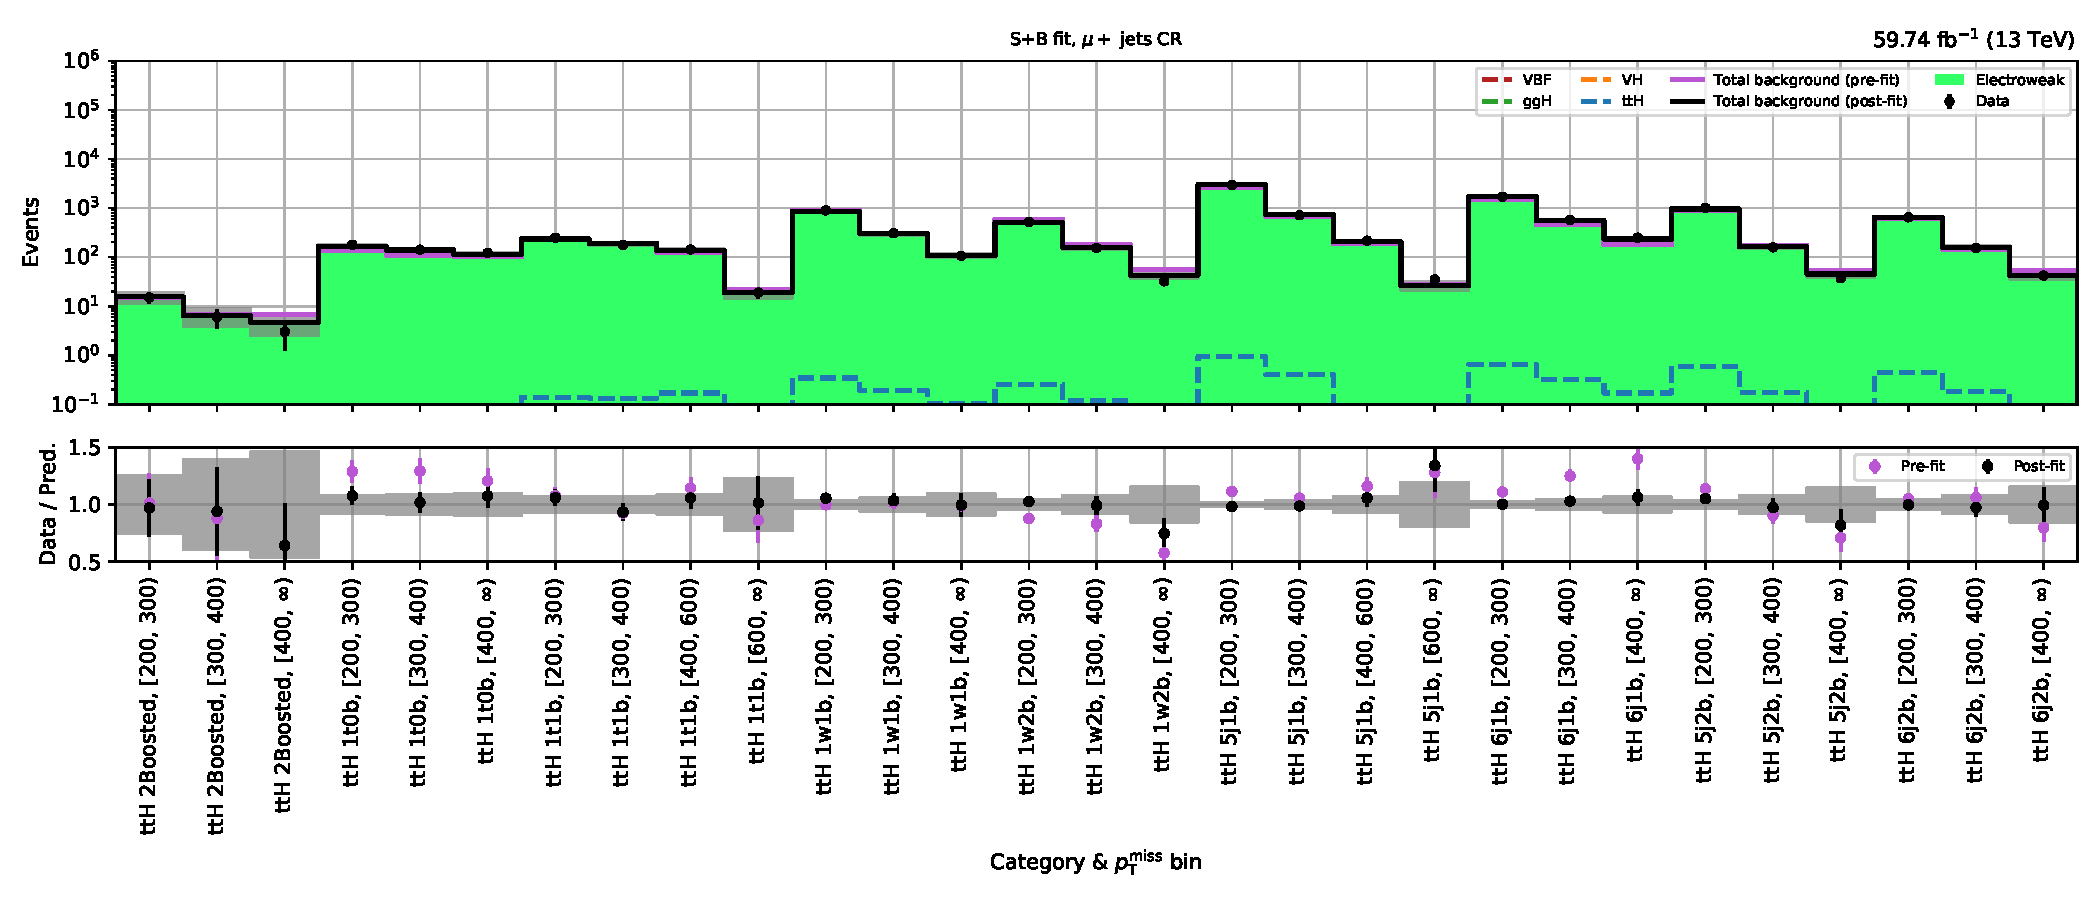
\includegraphics[width=\textwidth]{chapters/higgstoinv/figures/mountain_ranges/2018/ttH/Wmunu_tree_fit_s-abs_values_ttH_cats.pdf}
        \caption{\ttH --- \singleMuCr \gls{CR} (2018)}
    \end{subfigure}

    \begin{subfigure}[b]{0.66\textwidth}
        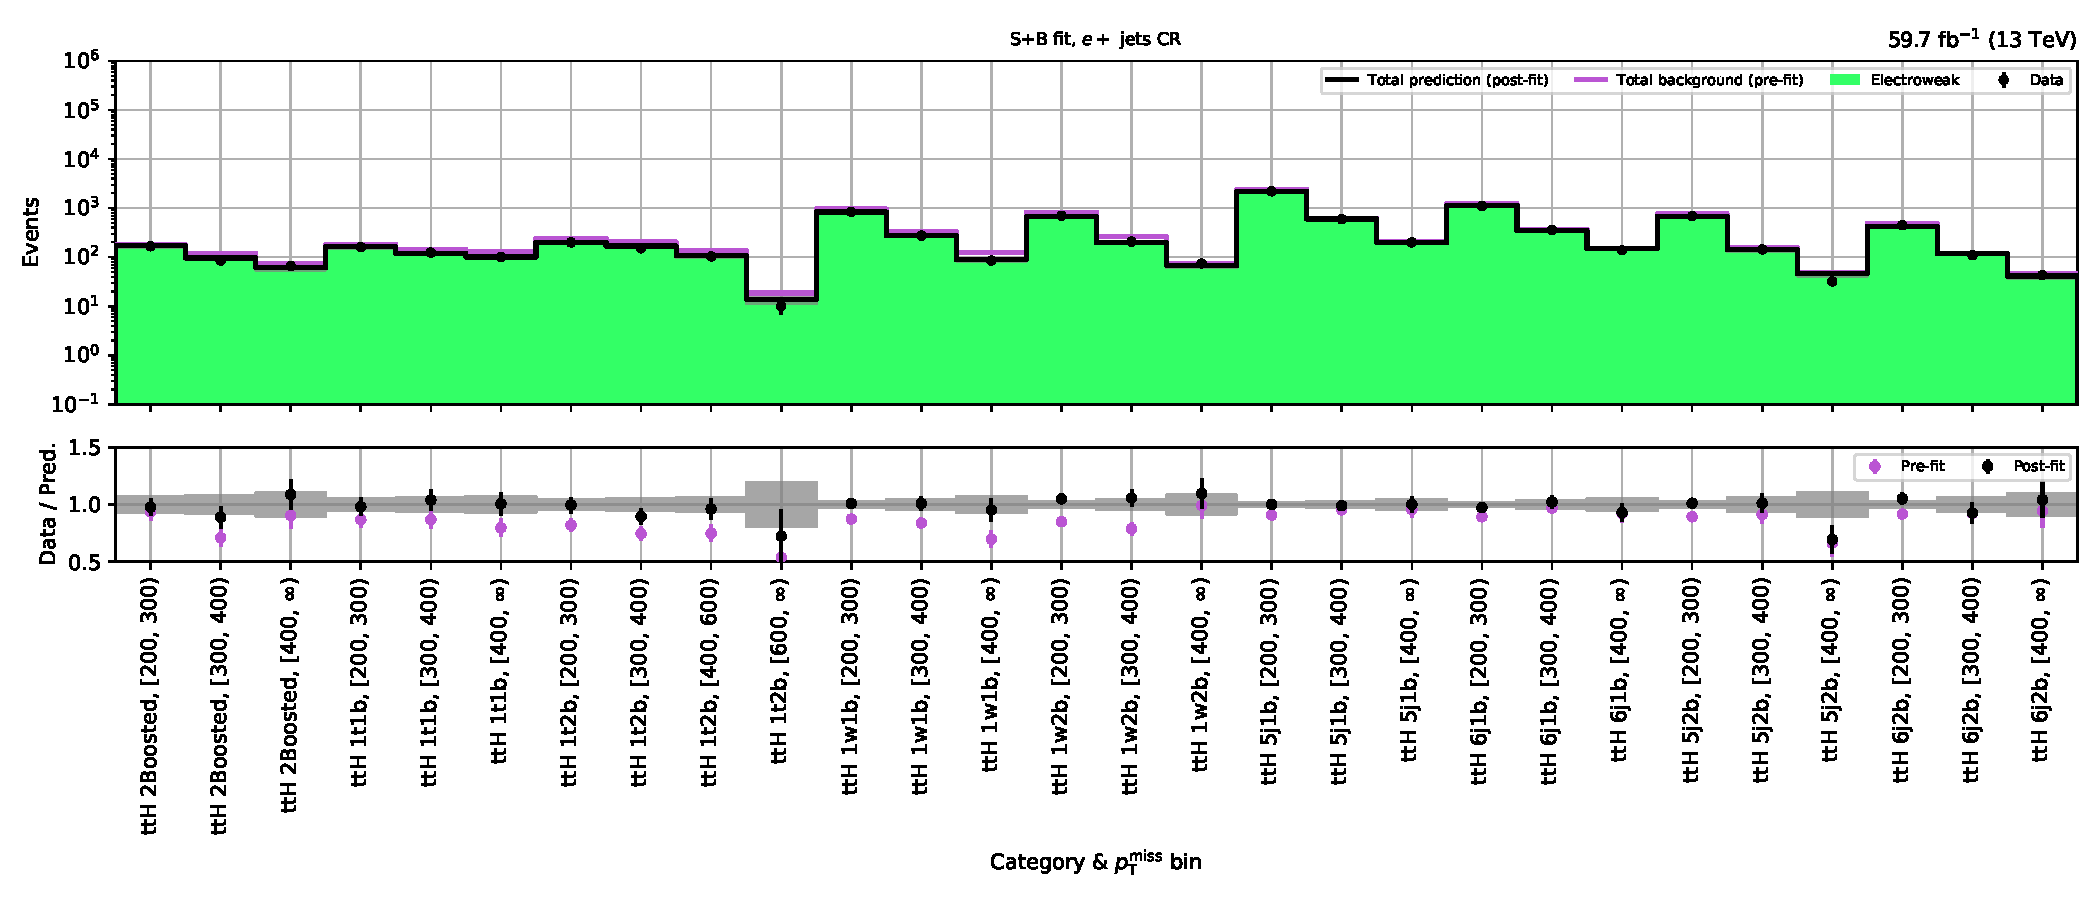
\includegraphics[width=\textwidth]{chapters/higgstoinv/figures/mountain_ranges/2018/ttH/Wenu_tree_fit_s-abs_values_ttH_cats.pdf}
        \caption{\ttH --- \singleEleCr \gls{CR} (2018)}
    \end{subfigure}

    \begin{subfigure}[b]{0.66\textwidth}
        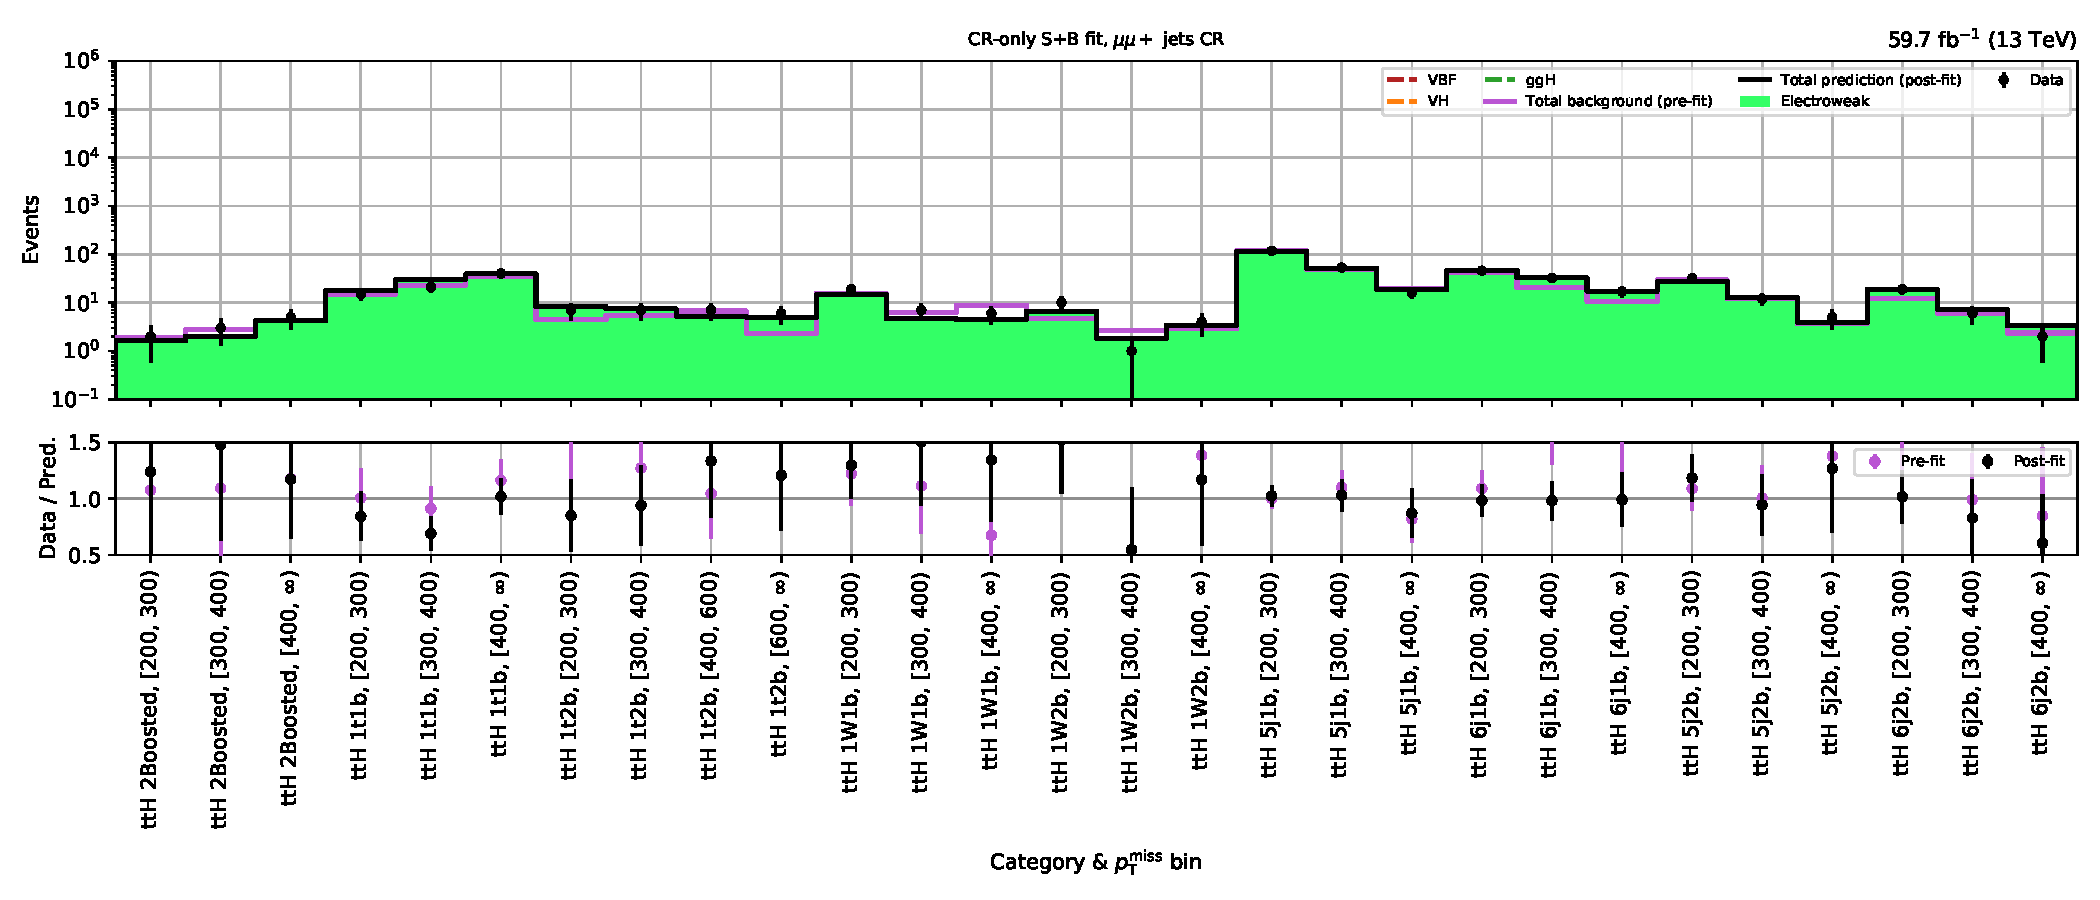
\includegraphics[width=\textwidth]{chapters/higgstoinv/figures/mountain_ranges/2018/ttH/Zmumu_tree_fit_s-abs_values_ttH_cats.pdf}
        \caption{\ttH --- \doubleMuCr \gls{CR} (2018)}
    \end{subfigure}

    \begin{subfigure}[b]{0.66\textwidth}
        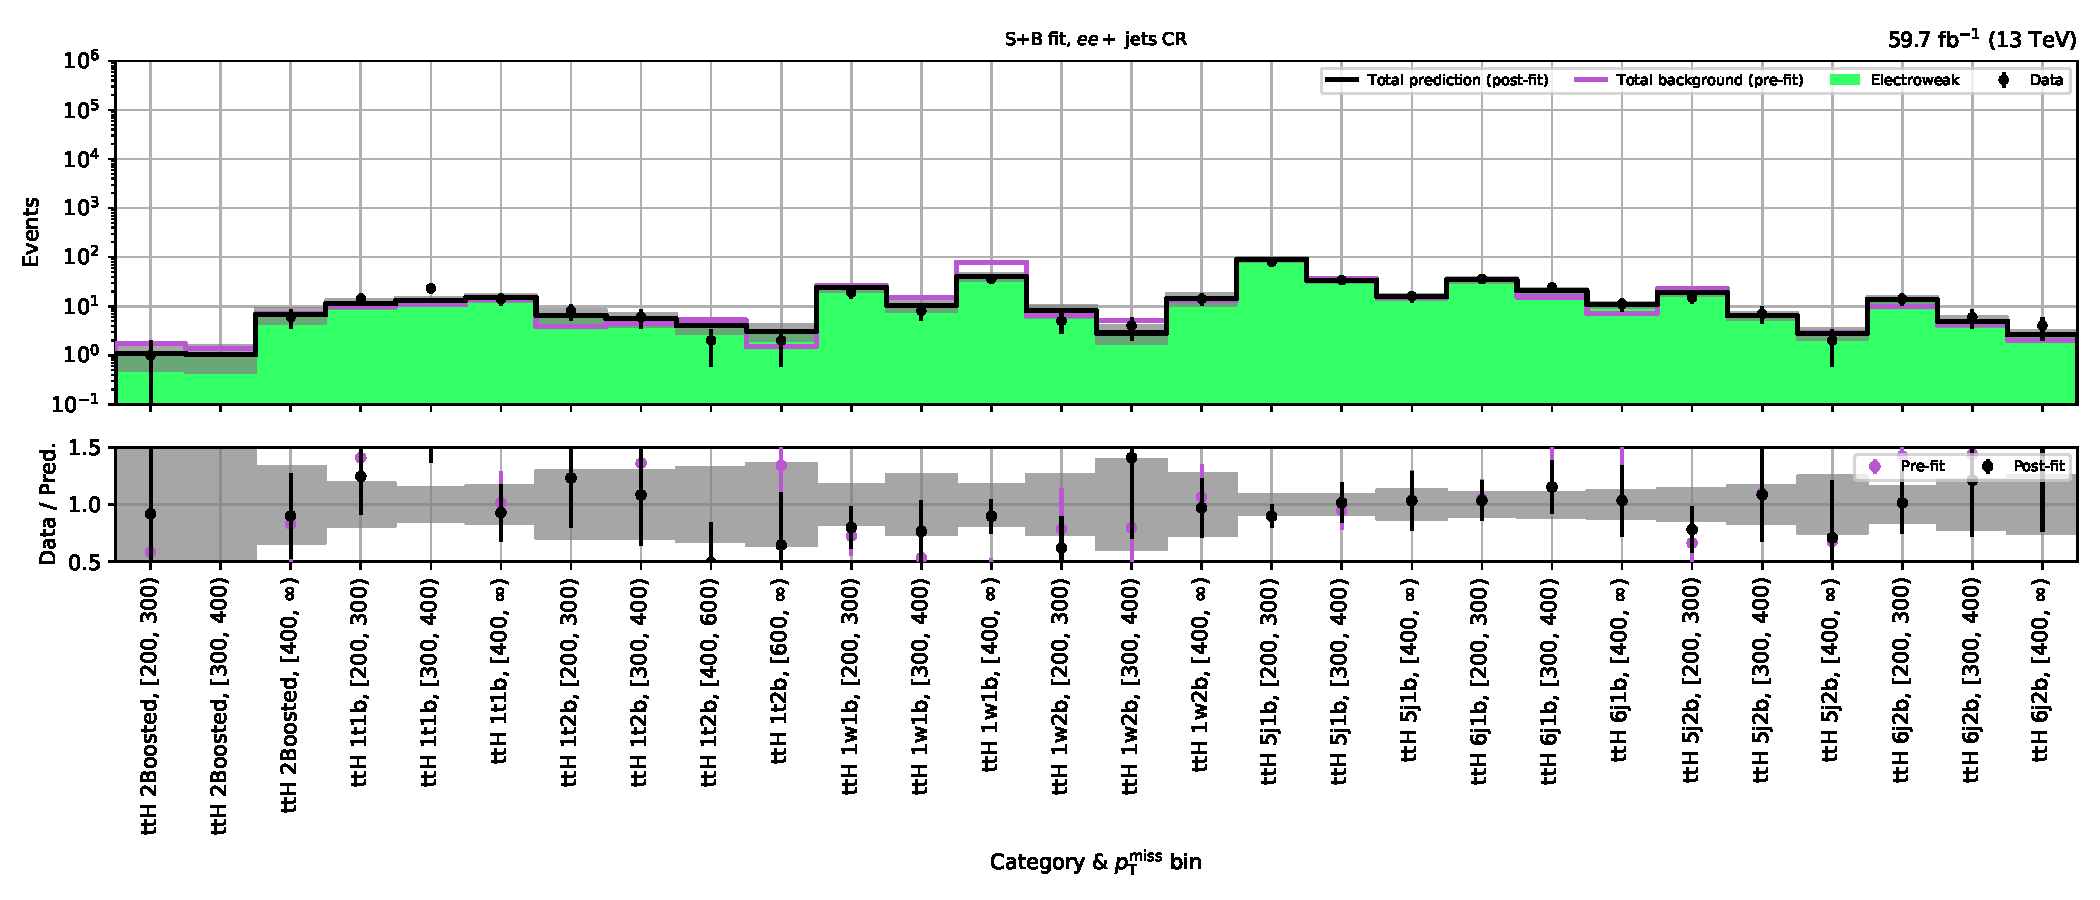
\includegraphics[width=\textwidth]{chapters/higgstoinv/figures/mountain_ranges/2018/ttH/Zee_tree_fit_s-abs_values_ttH_cats.pdf}
        \caption{\ttH --- \doubleEleCr \gls{CR} (2018)}
    \end{subfigure}
    \caption[Post-fit yields for each \ttH subcategory and \ptmiss bin in the lepton control regions for the 2018 dataset]{Post-fit yields for each \ttH subcategory and \ptmiss bin in the lepton \glspl{CR} for the 2018 dataset. The total background pre-fit and post-fit is compared in the lower panel of each subfigure.}
    \label{fig:htoinv_mountain_range_ttH_2018_CRs}
\end{figure}



%=========================================================


\section{Post-fit distributions of the control regions in the \texorpdfstring{\VH}{VH} category}
\label{sec:pre_post_fit_plots_VH_CRs}

\begin{figure}[htbp]
    \centering
    \begin{subfigure}[b]{0.51\textwidth}
        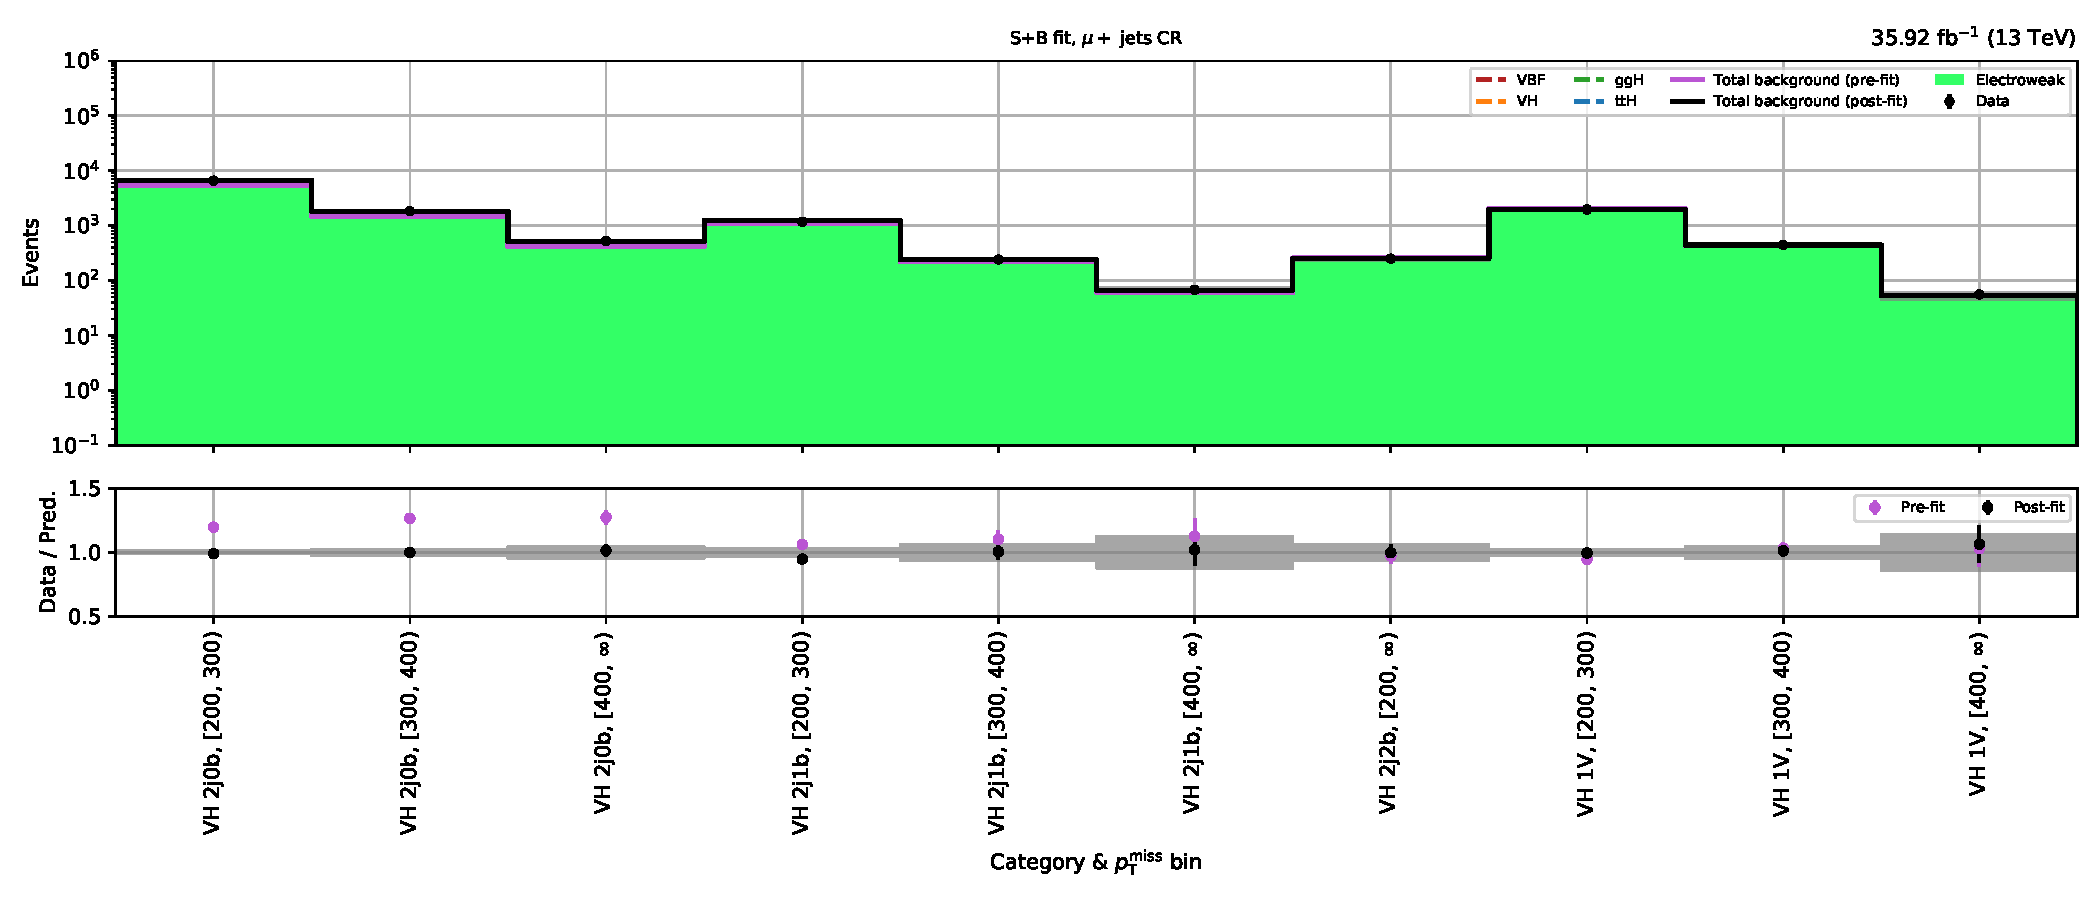
\includegraphics[width=\textwidth]{chapters/higgstoinv/figures/mountain_ranges/2016/VH/Wmunu_tree_fit_s-abs_values_VH_cats.pdf}
        \caption{\VH --- \singleMuCr \gls{CR} (2016)}
    \end{subfigure}

    \begin{subfigure}[b]{0.51\textwidth}
        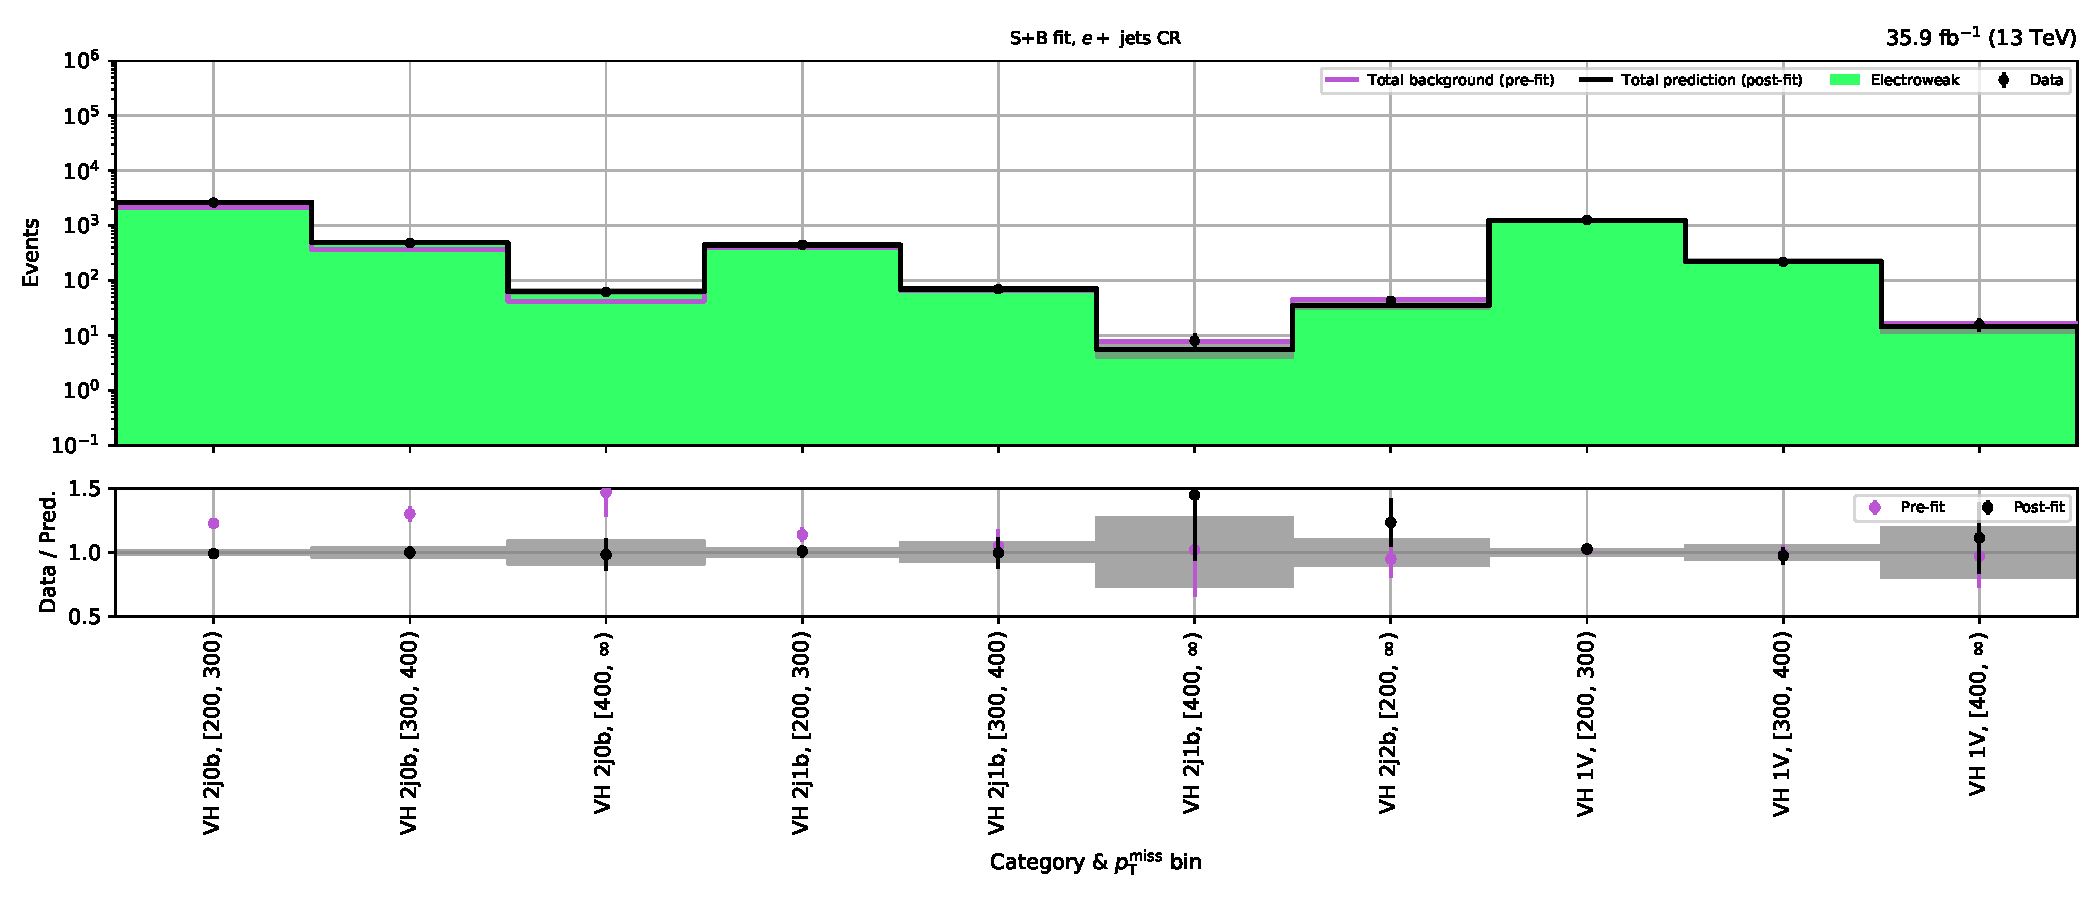
\includegraphics[width=\textwidth]{chapters/higgstoinv/figures/mountain_ranges/2016/VH/Wenu_tree_fit_s-abs_values_VH_cats.pdf}
        \caption{\VH --- \singleEleCr \gls{CR} (2016)}
    \end{subfigure}

    \begin{subfigure}[b]{0.51\textwidth}
        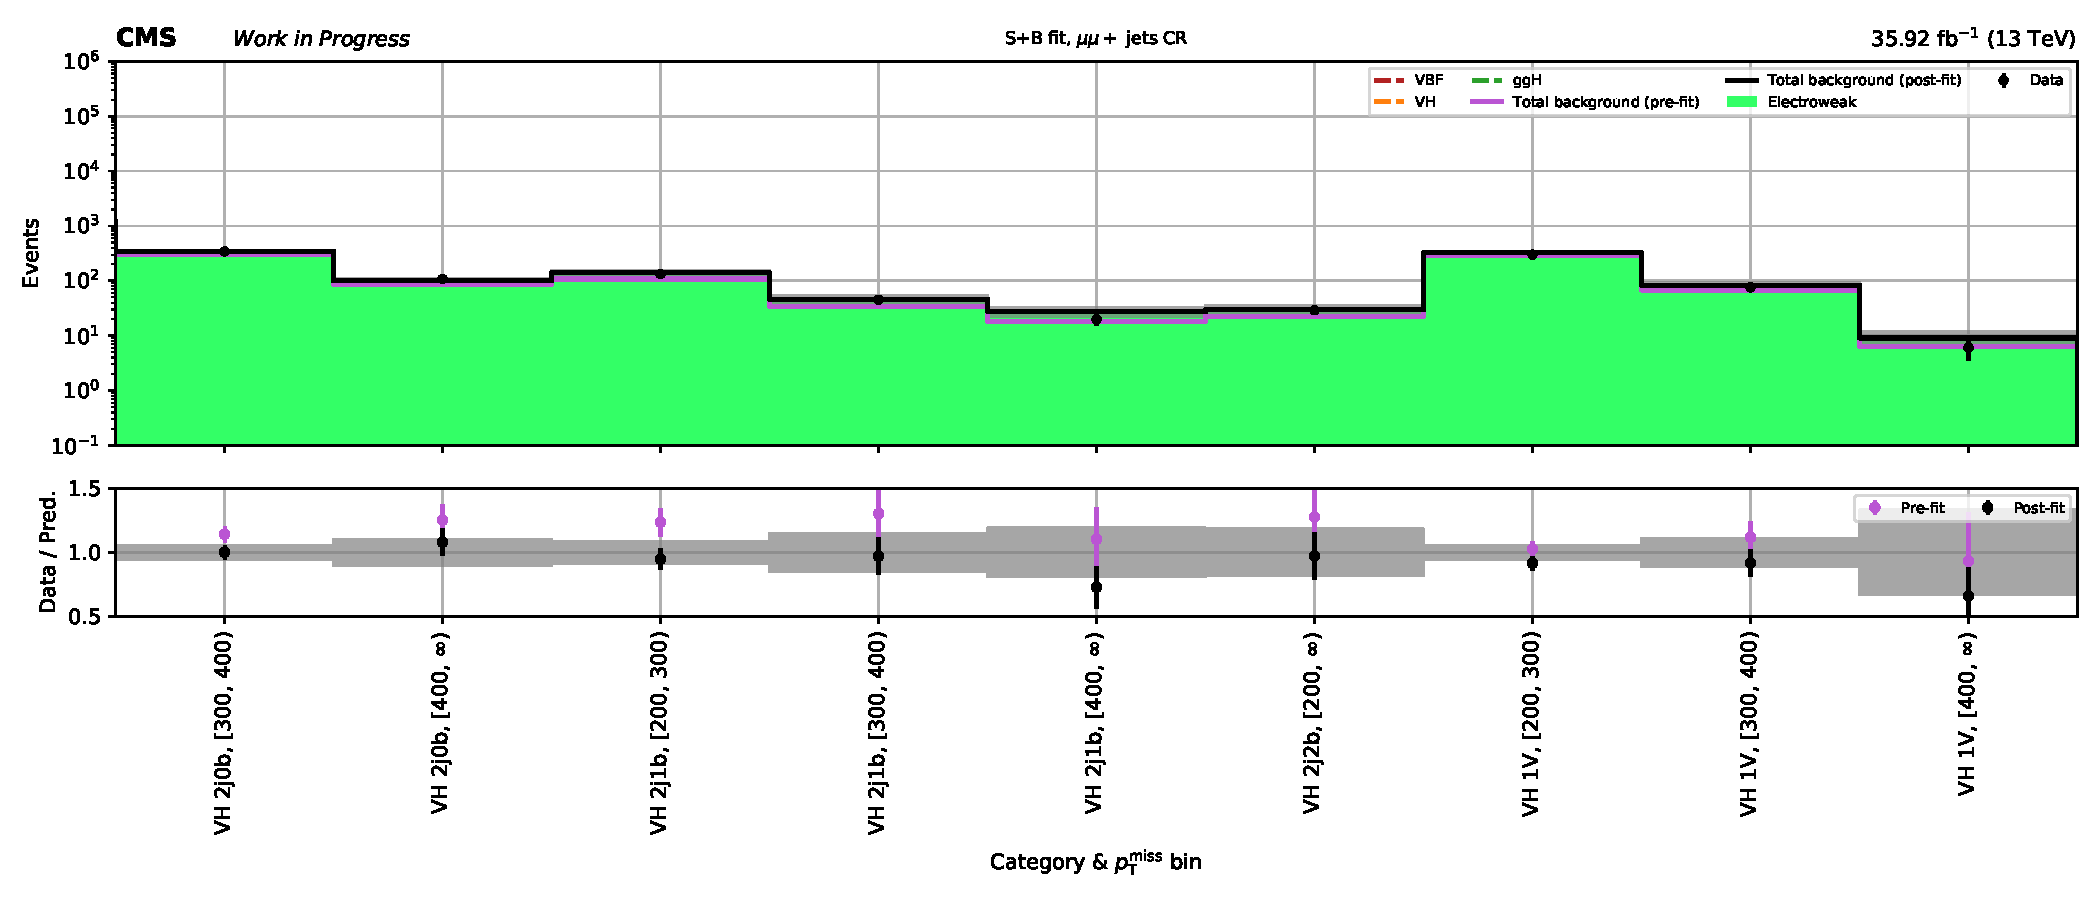
\includegraphics[width=\textwidth]{chapters/higgstoinv/figures/mountain_ranges/2016/VH/Zmumu_tree_fit_s-abs_values_VH_cats.pdf}
        \caption{\VH --- \doubleMuCr \gls{CR} (2016)}
    \end{subfigure}

    \begin{subfigure}[b]{0.51\textwidth}
        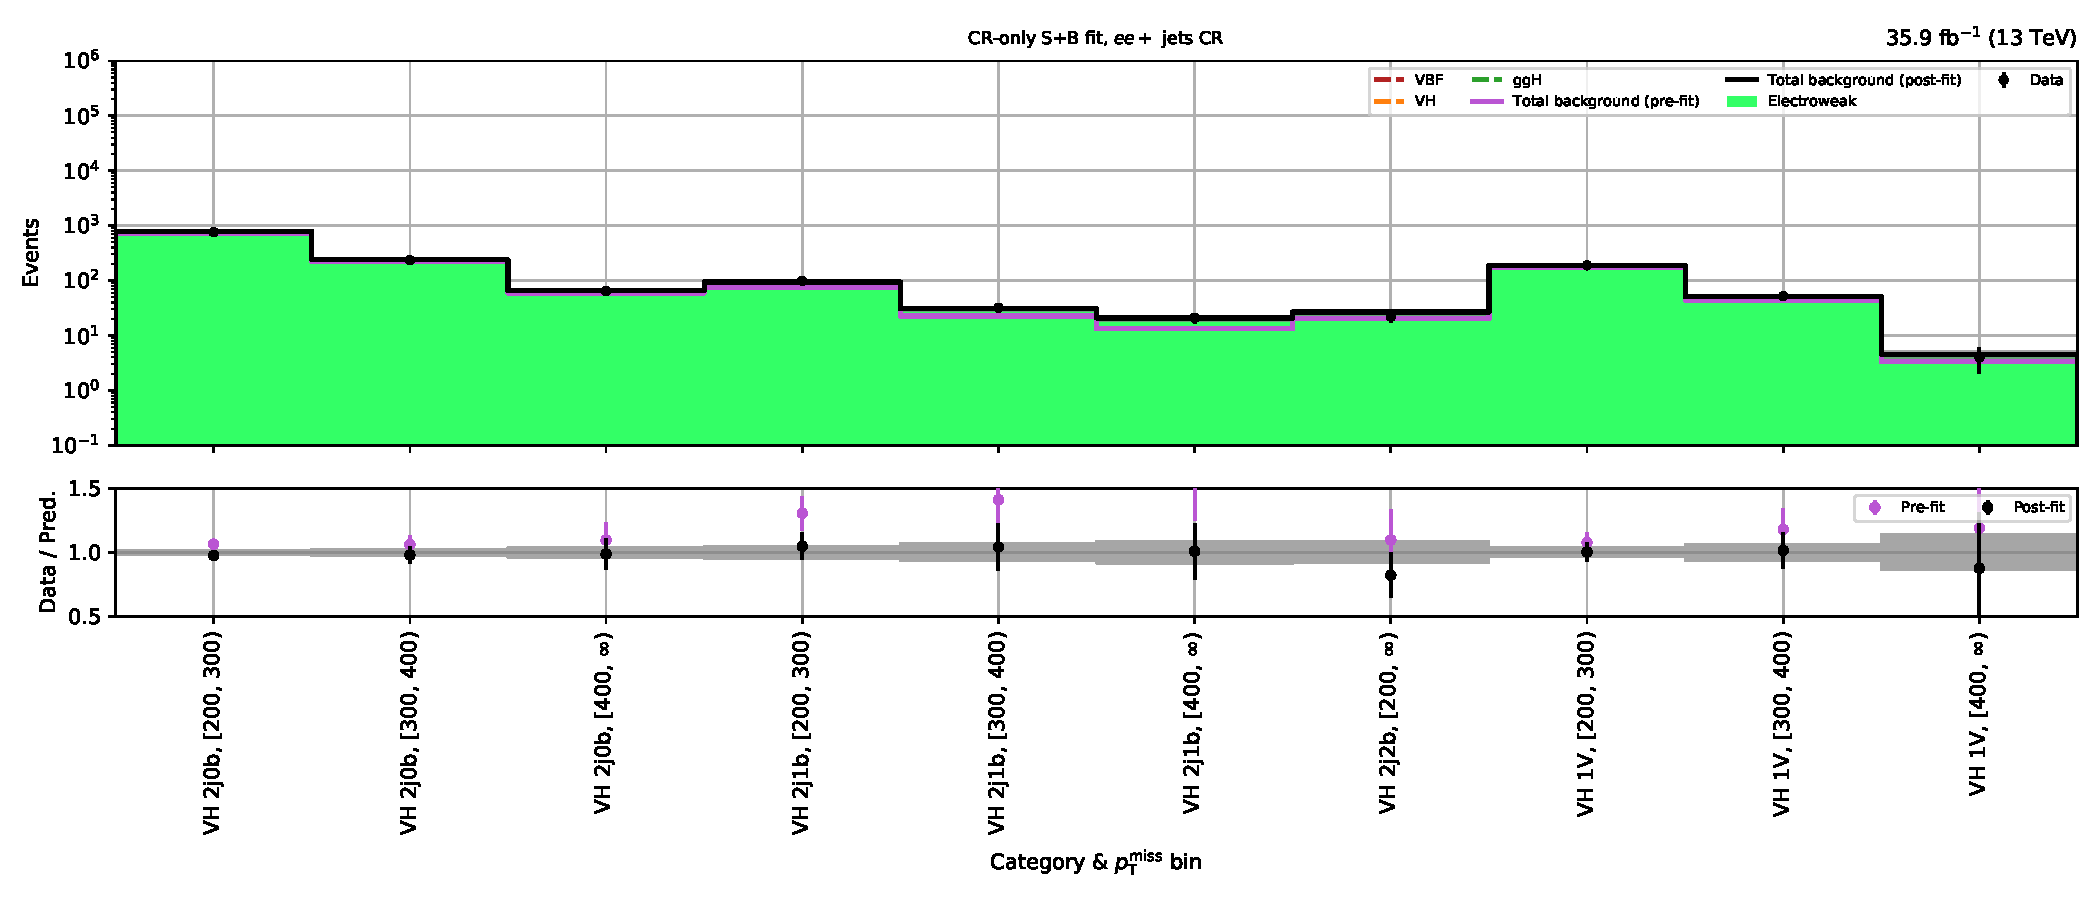
\includegraphics[width=\textwidth]{chapters/higgstoinv/figures/mountain_ranges/2016/VH/Zee_tree_fit_s-abs_values_VH_cats.pdf}
        \caption{\VH --- \doubleEleCr \gls{CR} (2016)}
    \end{subfigure}

    \begin{subfigure}[b]{0.51\textwidth}
        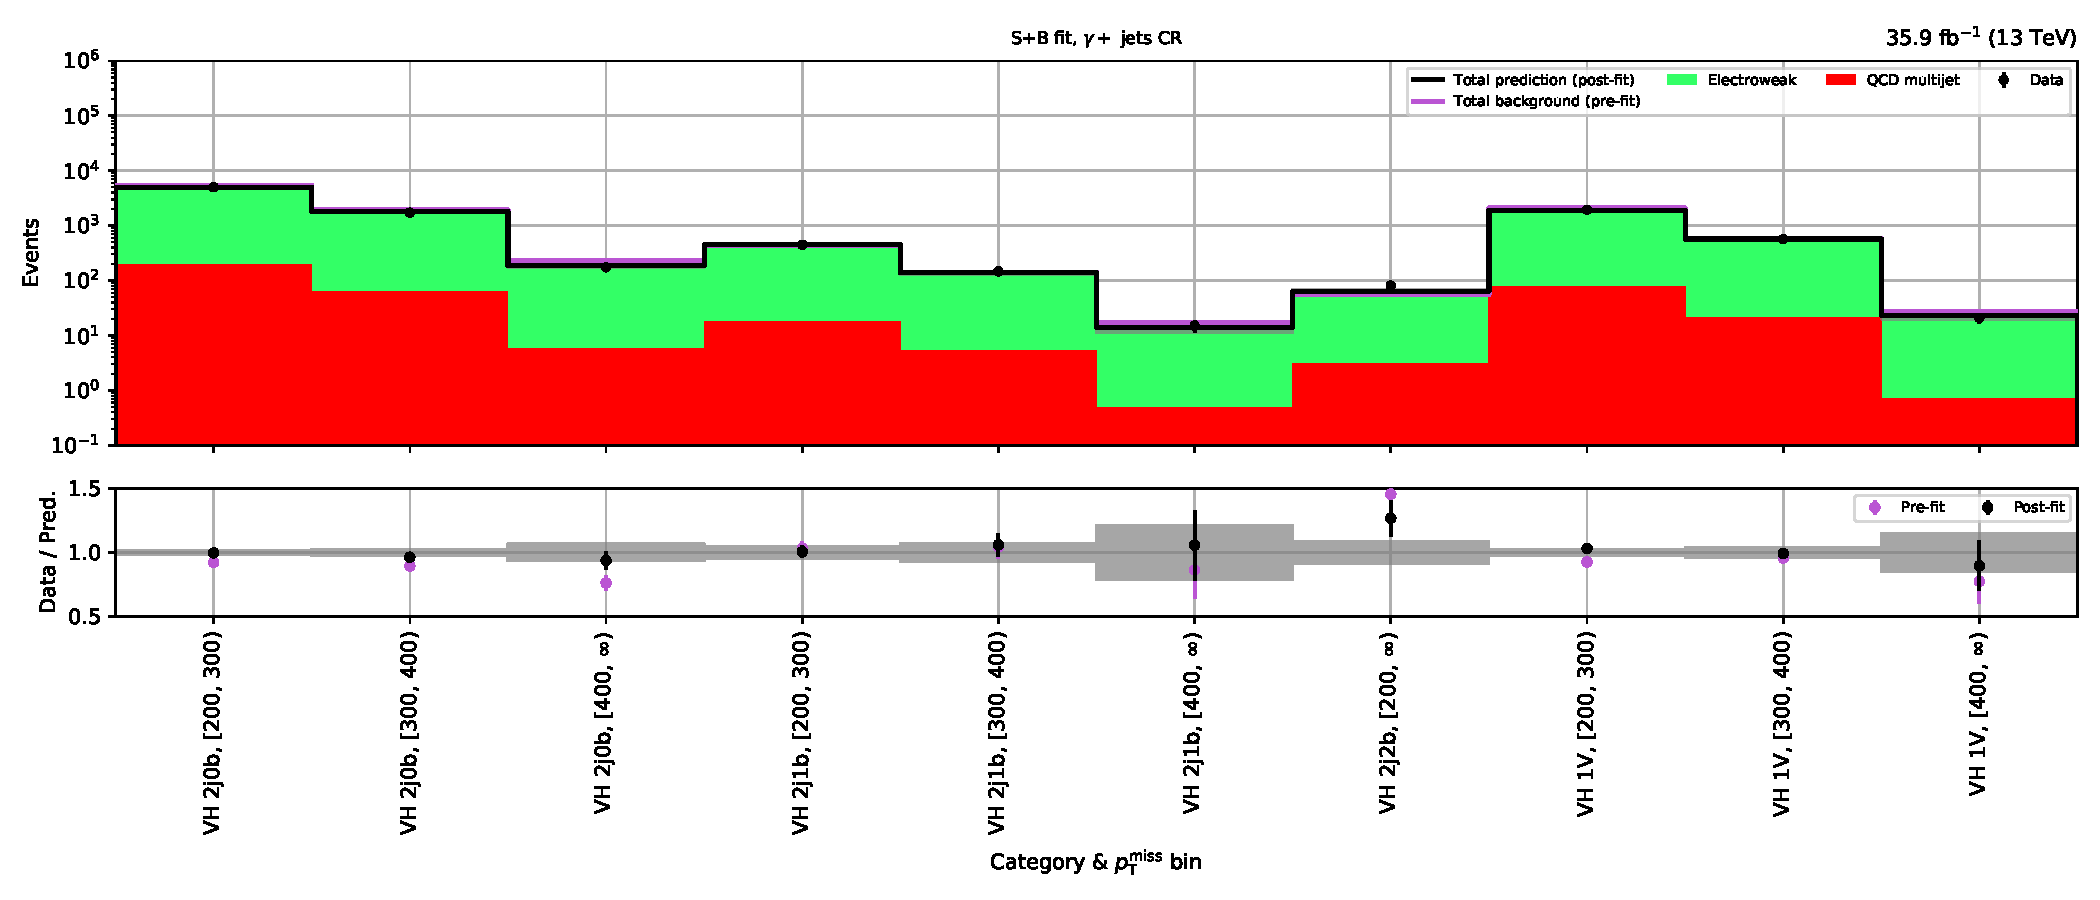
\includegraphics[width=\textwidth]{chapters/higgstoinv/figures/mountain_ranges/2016/VH/Photon_tree_fit_s-abs_values_VH_cats.pdf}
        \caption{\VH --- \singlePhotonCr \gls{CR} (2016)}
    \end{subfigure}
    \caption[Post-fit yields for each \VH subcategory and \ptmiss bin in the lepton and photon control regions for the 2016 dataset]{Post-fit yields for each \VH subcategory and \ptmiss bin in the lepton and photon \glspl{CR} for the 2016 dataset. The total background pre-fit and post-fit is compared in the lower panel of each subfigure.}
    \label{fig:htoinv_mountain_range_VH_2016_CRs}
\end{figure}

\begin{figure}[htbp]
    \centering
    \begin{subfigure}[b]{0.66\textwidth}
        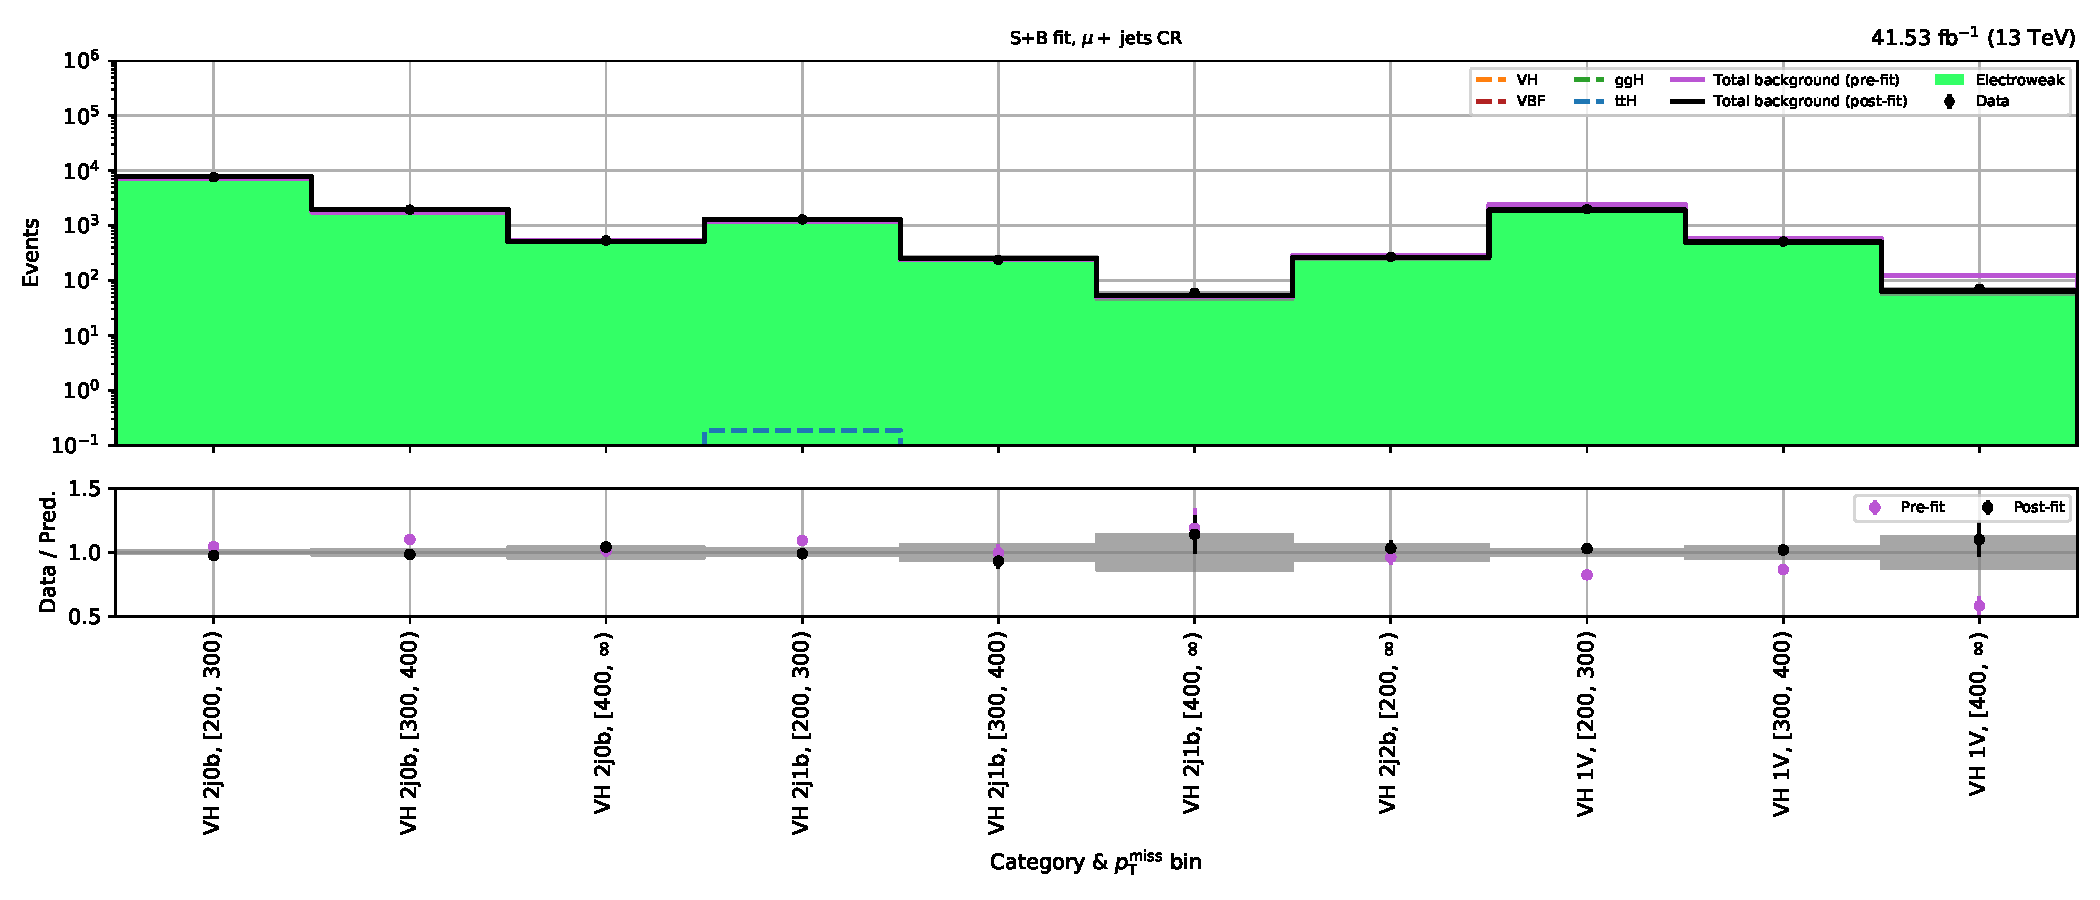
\includegraphics[width=\textwidth]{chapters/higgstoinv/figures/mountain_ranges/2017/VH/Wmunu_tree_fit_s-abs_values_VH_cats.pdf}
        \caption{\VH --- \singleMuCr \gls{CR} (2017)}
    \end{subfigure}

    \begin{subfigure}[b]{0.66\textwidth}
        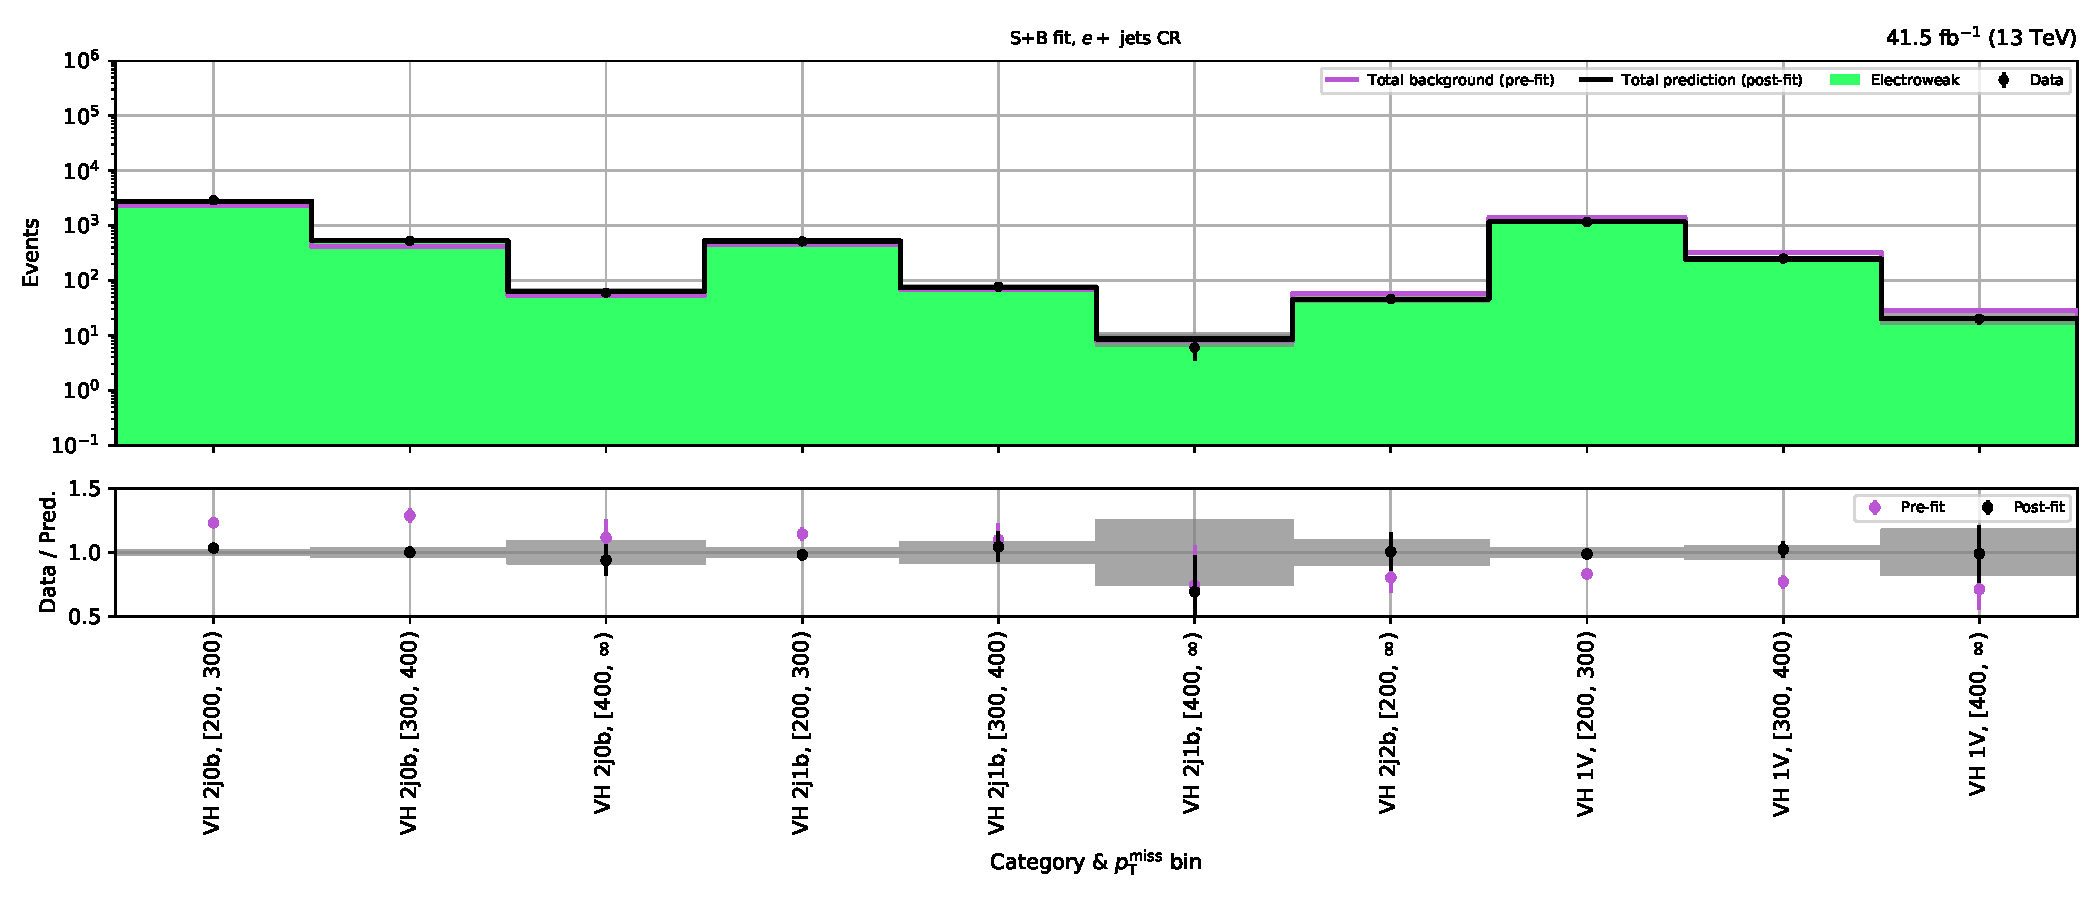
\includegraphics[width=\textwidth]{chapters/higgstoinv/figures/mountain_ranges/2017/VH/Wenu_tree_fit_s-abs_values_VH_cats.pdf}
        \caption{\VH --- \singleEleCr \gls{CR} (2017)}
    \end{subfigure}

    \begin{subfigure}[b]{0.66\textwidth}
        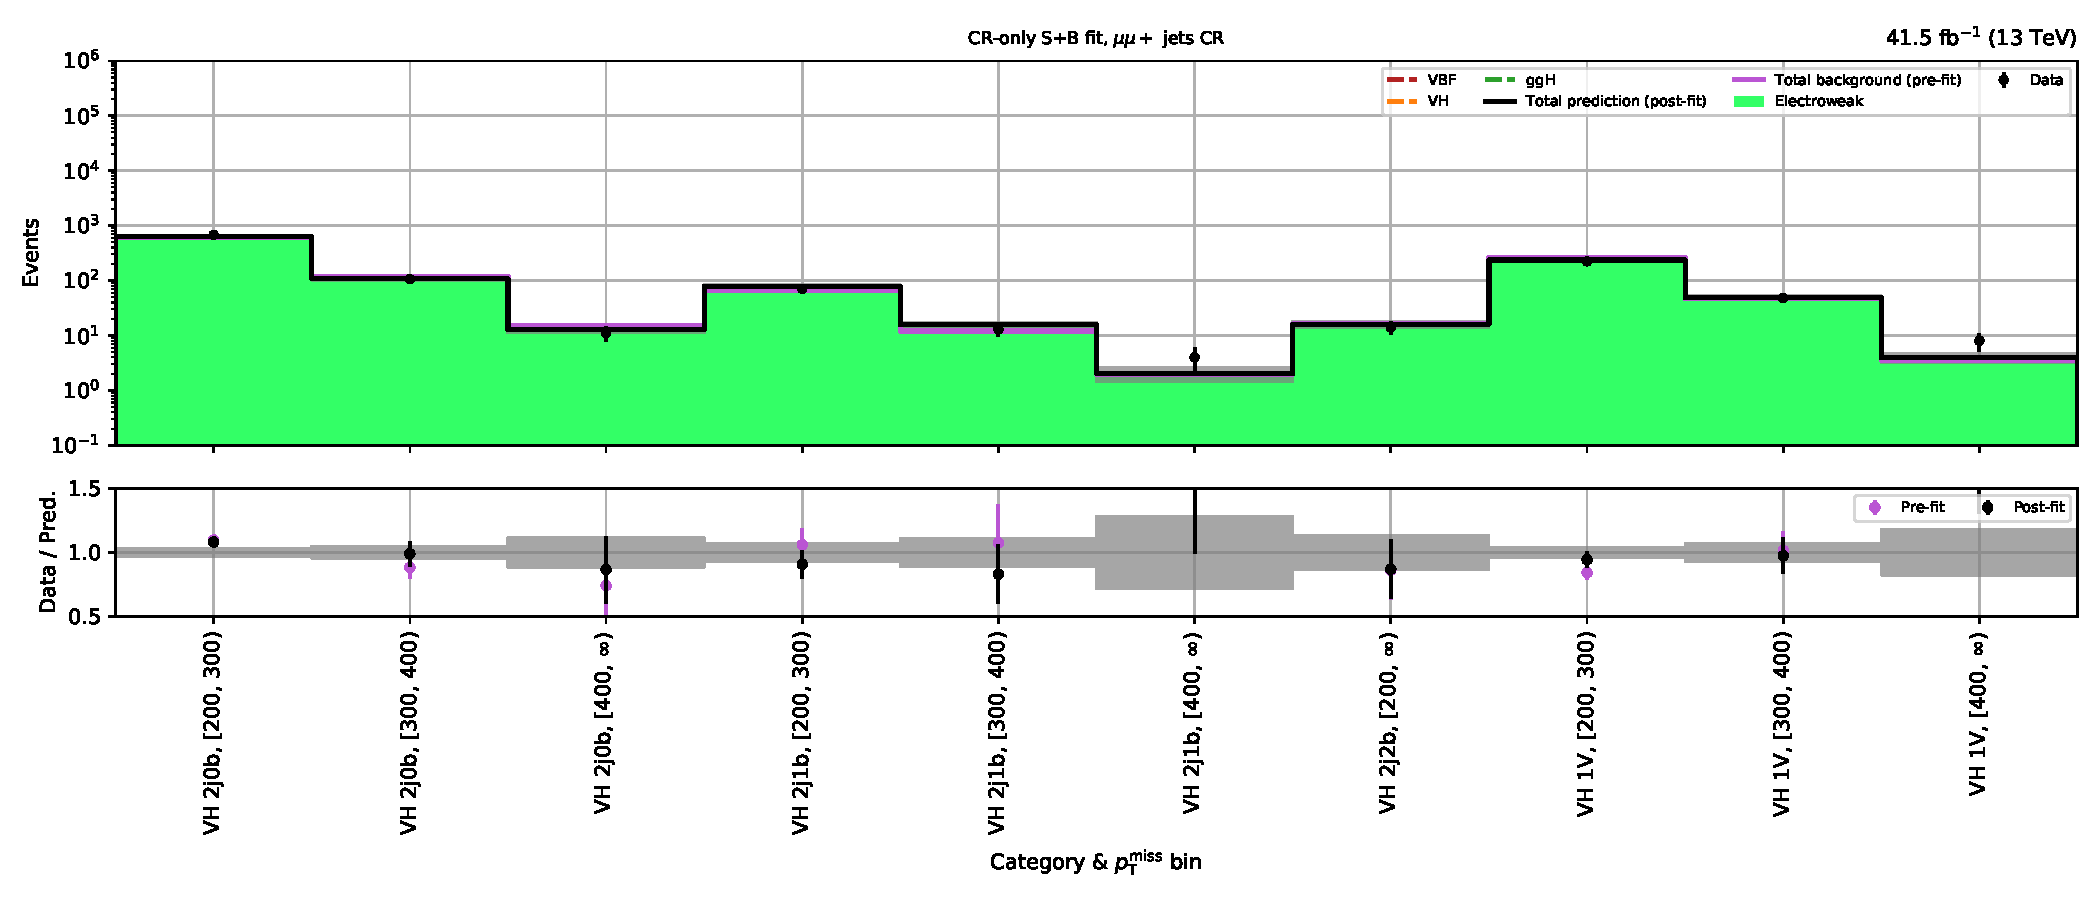
\includegraphics[width=\textwidth]{chapters/higgstoinv/figures/mountain_ranges/2017/VH/Zmumu_tree_fit_s-abs_values_VH_cats.pdf}
        \caption{\VH --- \doubleMuCr \gls{CR} (2017)}
    \end{subfigure}

    \begin{subfigure}[b]{0.66\textwidth}
        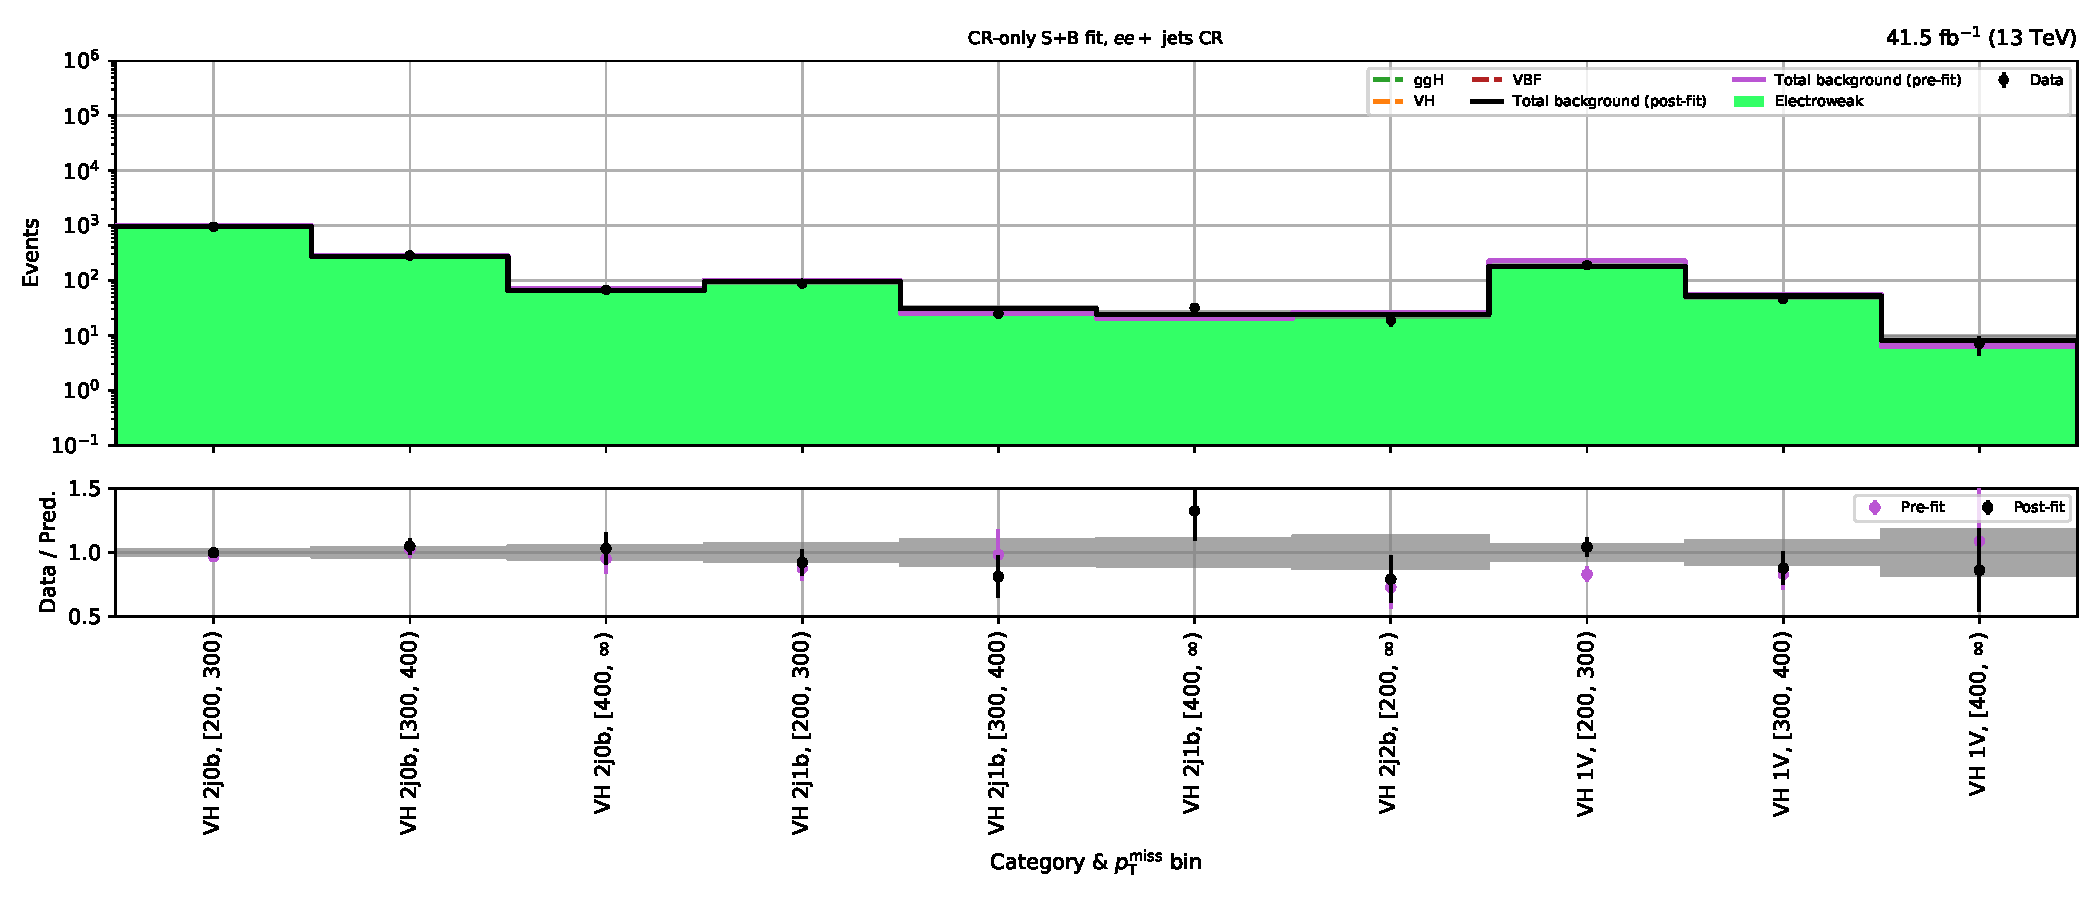
\includegraphics[width=\textwidth]{chapters/higgstoinv/figures/mountain_ranges/2017/VH/Zee_tree_fit_s-abs_values_VH_cats.pdf}
        \caption{\VH --- \doubleEleCr \gls{CR} (2017)}
    \end{subfigure}

    \begin{subfigure}[b]{0.66\textwidth}
        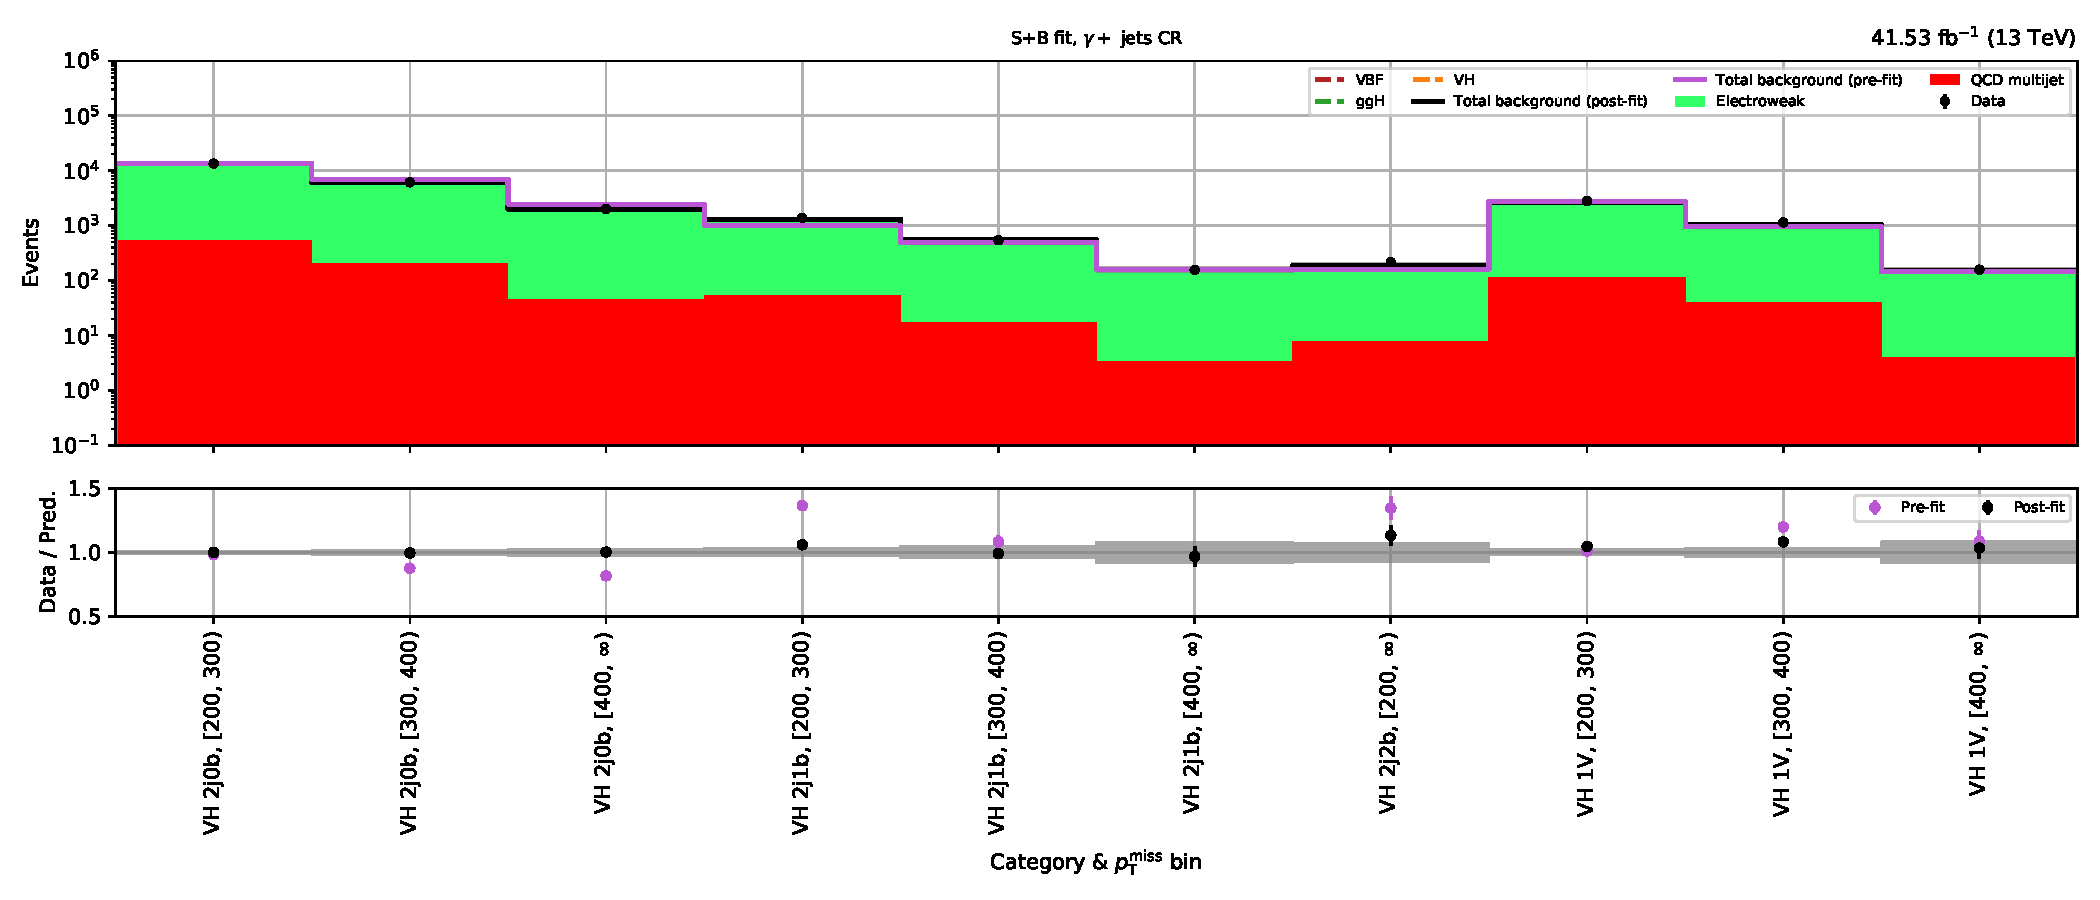
\includegraphics[width=\textwidth]{chapters/higgstoinv/figures/mountain_ranges/2017/VH/Photon_tree_fit_s-abs_values_VH_cats.pdf}
        \caption{\VH --- \singlePhotonCr \gls{CR} (2017)}
    \end{subfigure}
    \caption[Post-fit yields for each \VH subcategory and \ptmiss bin in the lepton and photon control regions for the 2017 dataset]{Post-fit yields for each \VH subcategory and \ptmiss bin in the lepton and photon \glspl{CR} for the 2017 dataset. The total background pre-fit and post-fit is compared in the lower panel of each subfigure.}
    \label{fig:htoinv_mountain_range_VH_2017_CRs}
\end{figure}

\begin{figure}[htbp]
    \centering
    \begin{subfigure}[b]{0.66\textwidth}
        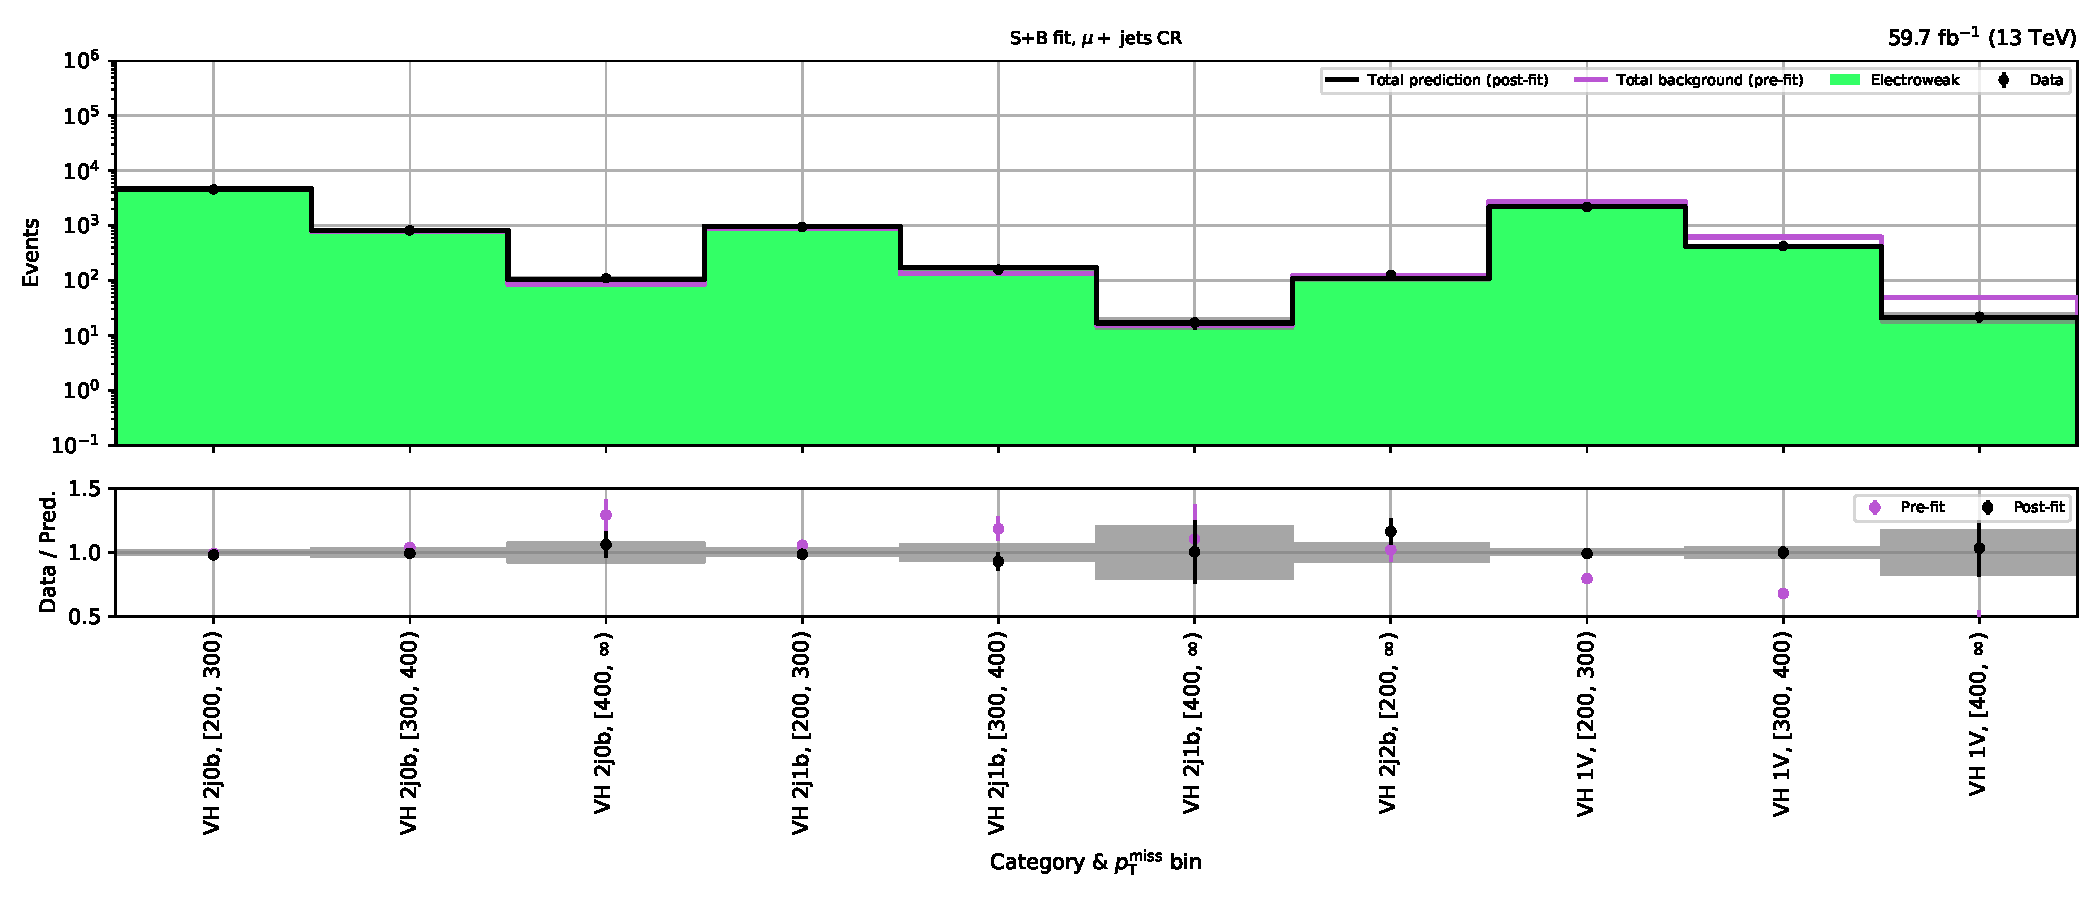
\includegraphics[width=\textwidth]{chapters/higgstoinv/figures/mountain_ranges/2018/VH/Wmunu_tree_fit_s-abs_values_VH_cats.pdf}
        \caption{\VH --- \singleMuCr \gls{CR} (2018)}
    \end{subfigure}

    \begin{subfigure}[b]{0.66\textwidth}
        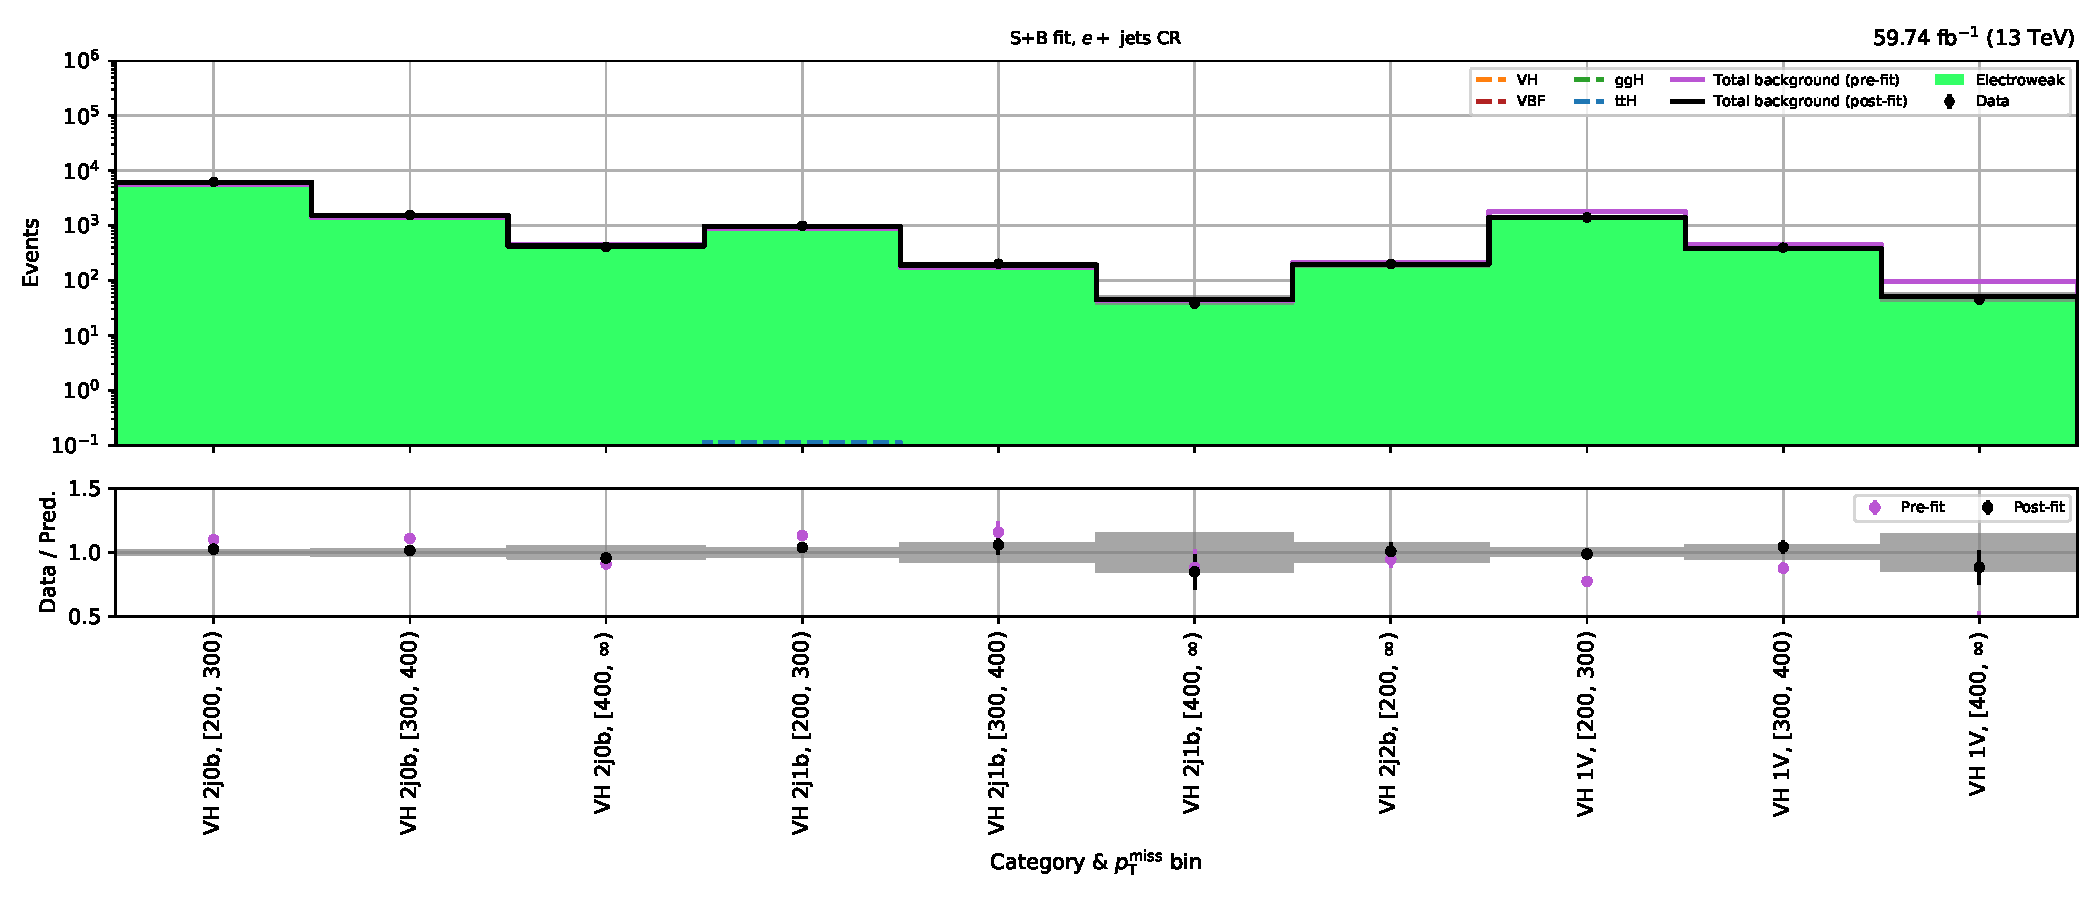
\includegraphics[width=\textwidth]{chapters/higgstoinv/figures/mountain_ranges/2018/VH/Wenu_tree_fit_s-abs_values_VH_cats.pdf}
        \caption{\VH --- \singleEleCr \gls{CR} (2018)}
    \end{subfigure}

    \begin{subfigure}[b]{0.66\textwidth}
        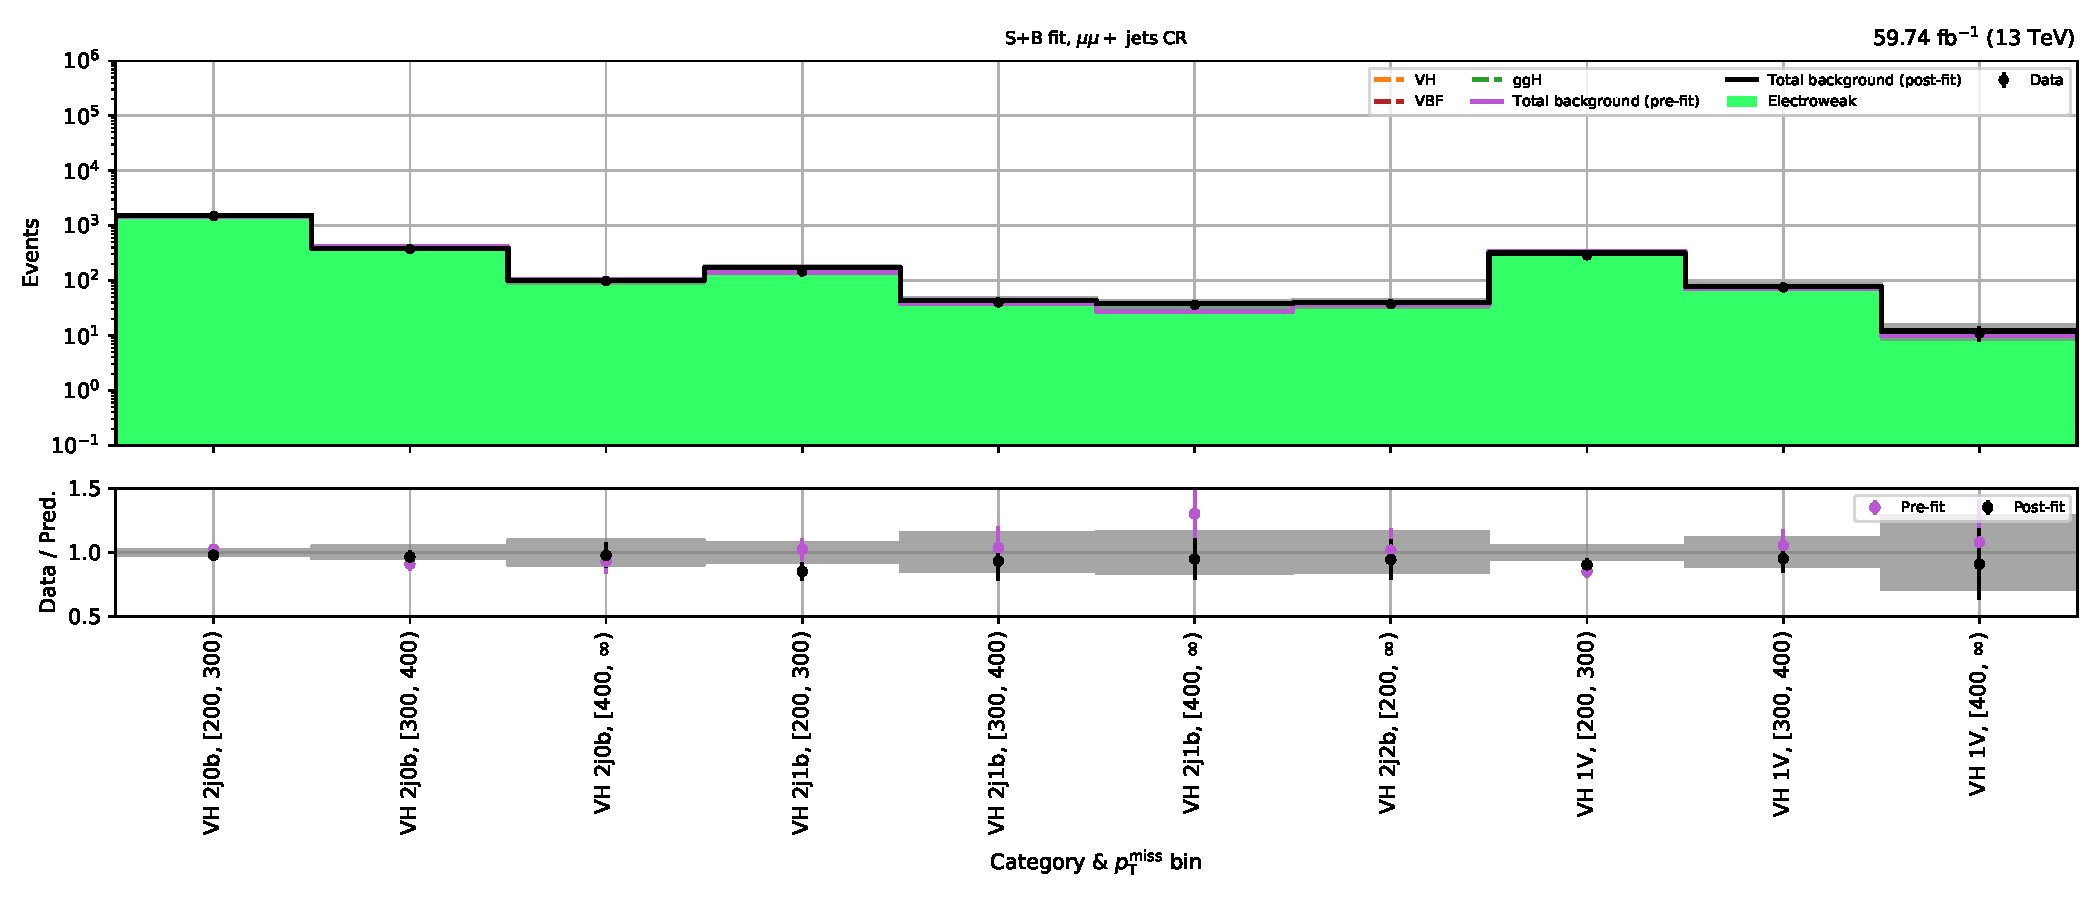
\includegraphics[width=\textwidth]{chapters/higgstoinv/figures/mountain_ranges/2018/VH/Zmumu_tree_fit_s-abs_values_VH_cats.pdf}
        \caption{\VH --- \doubleMuCr \gls{CR} (2018)}
    \end{subfigure}

    \begin{subfigure}[b]{0.66\textwidth}
        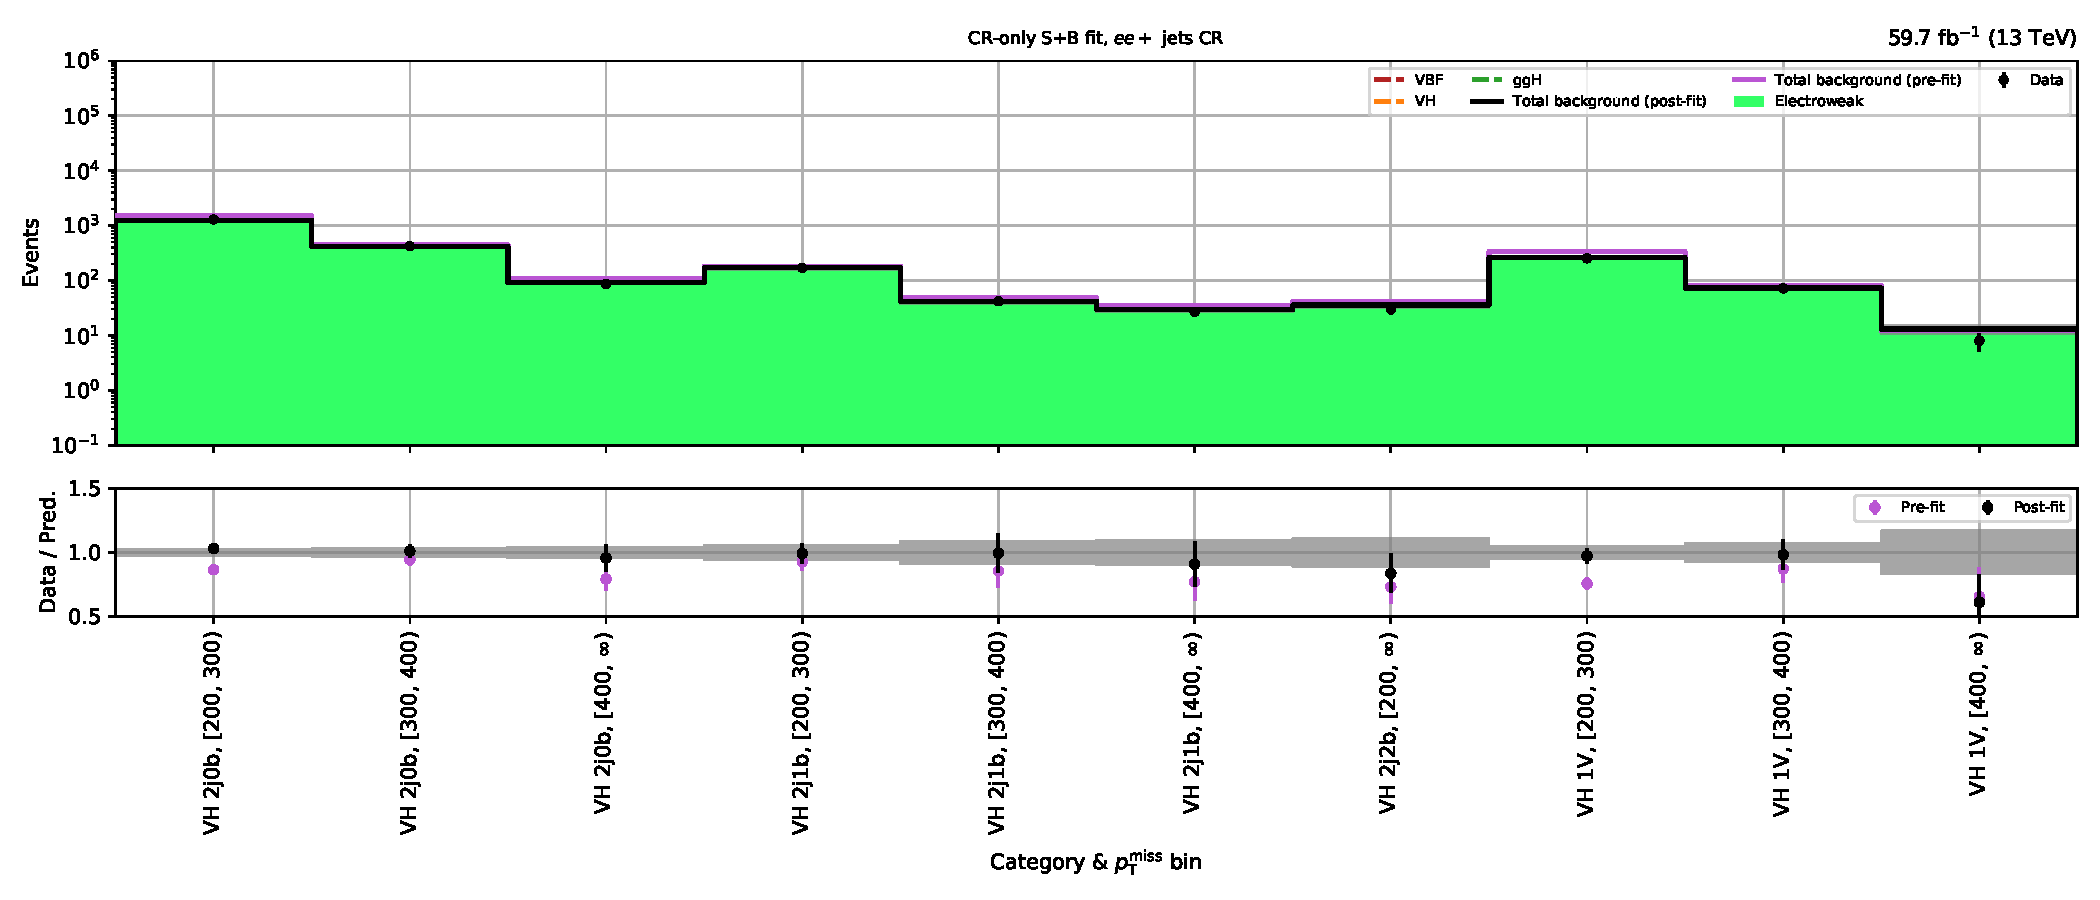
\includegraphics[width=\textwidth]{chapters/higgstoinv/figures/mountain_ranges/2018/VH/Zee_tree_fit_s-abs_values_VH_cats.pdf}
        \caption{\VH --- \doubleEleCr \gls{CR} (2018)}
    \end{subfigure}

    \begin{subfigure}[b]{0.66\textwidth}
        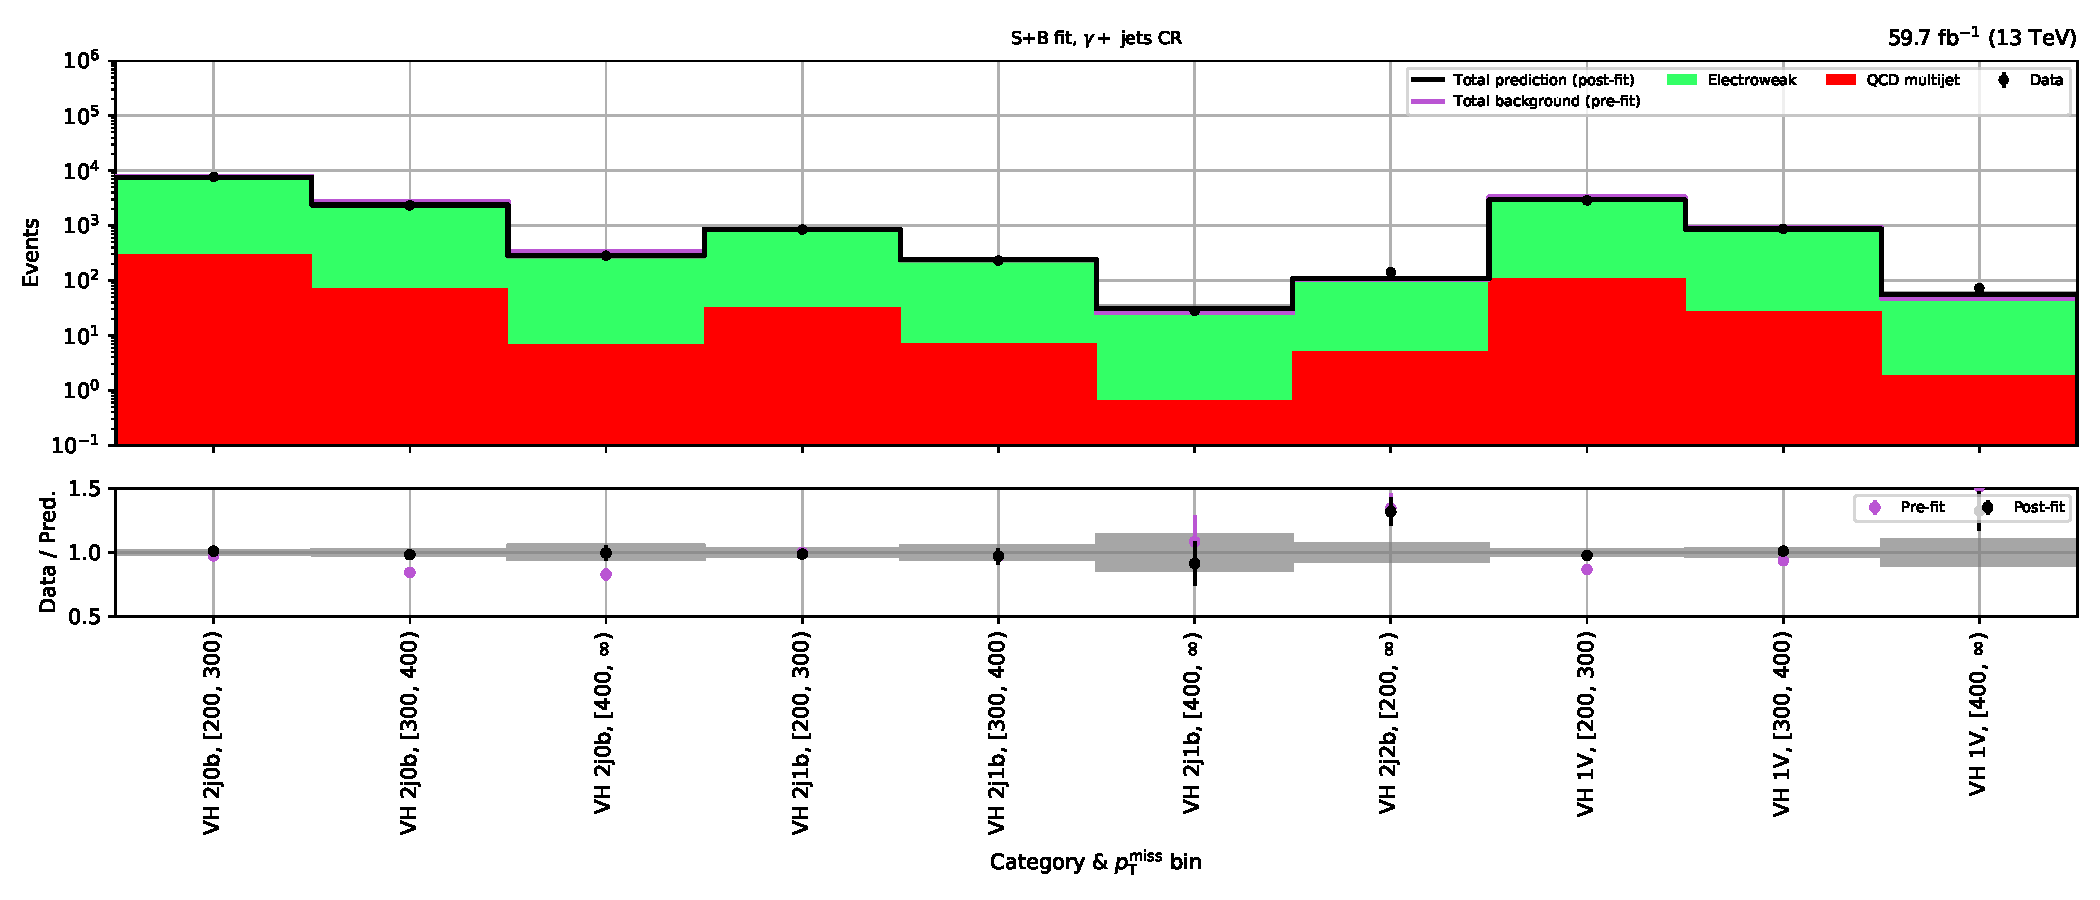
\includegraphics[width=\textwidth]{chapters/higgstoinv/figures/mountain_ranges/2018/VH/Photon_tree_fit_s-abs_values_VH_cats.pdf}
        \caption{\VH --- \singlePhotonCr \gls{CR} (2018)}
    \end{subfigure}
    \caption[Post-fit yields for each \VH subcategory and \ptmiss bin in the lepton and photon control regions for the 2018 dataset]{Post-fit yields for each \VH subcategory and \ptmiss bin in the lepton and photon \glspl{CR} for the 2018 dataset. The total background pre-fit and post-fit is compared in the lower panel of each subfigure.}
    \label{fig:htoinv_mountain_range_VH_2018_CRs}
\end{figure}


%=========================================================


\section{Post-fit distributions of the control regions in the \texorpdfstring{\ggH}{ggH} category}
\label{sec:pre_post_fit_plots_ggF_CRs}

\begin{figure}[htbp]
    \centering
    \begin{subfigure}[b]{0.66\textwidth}
        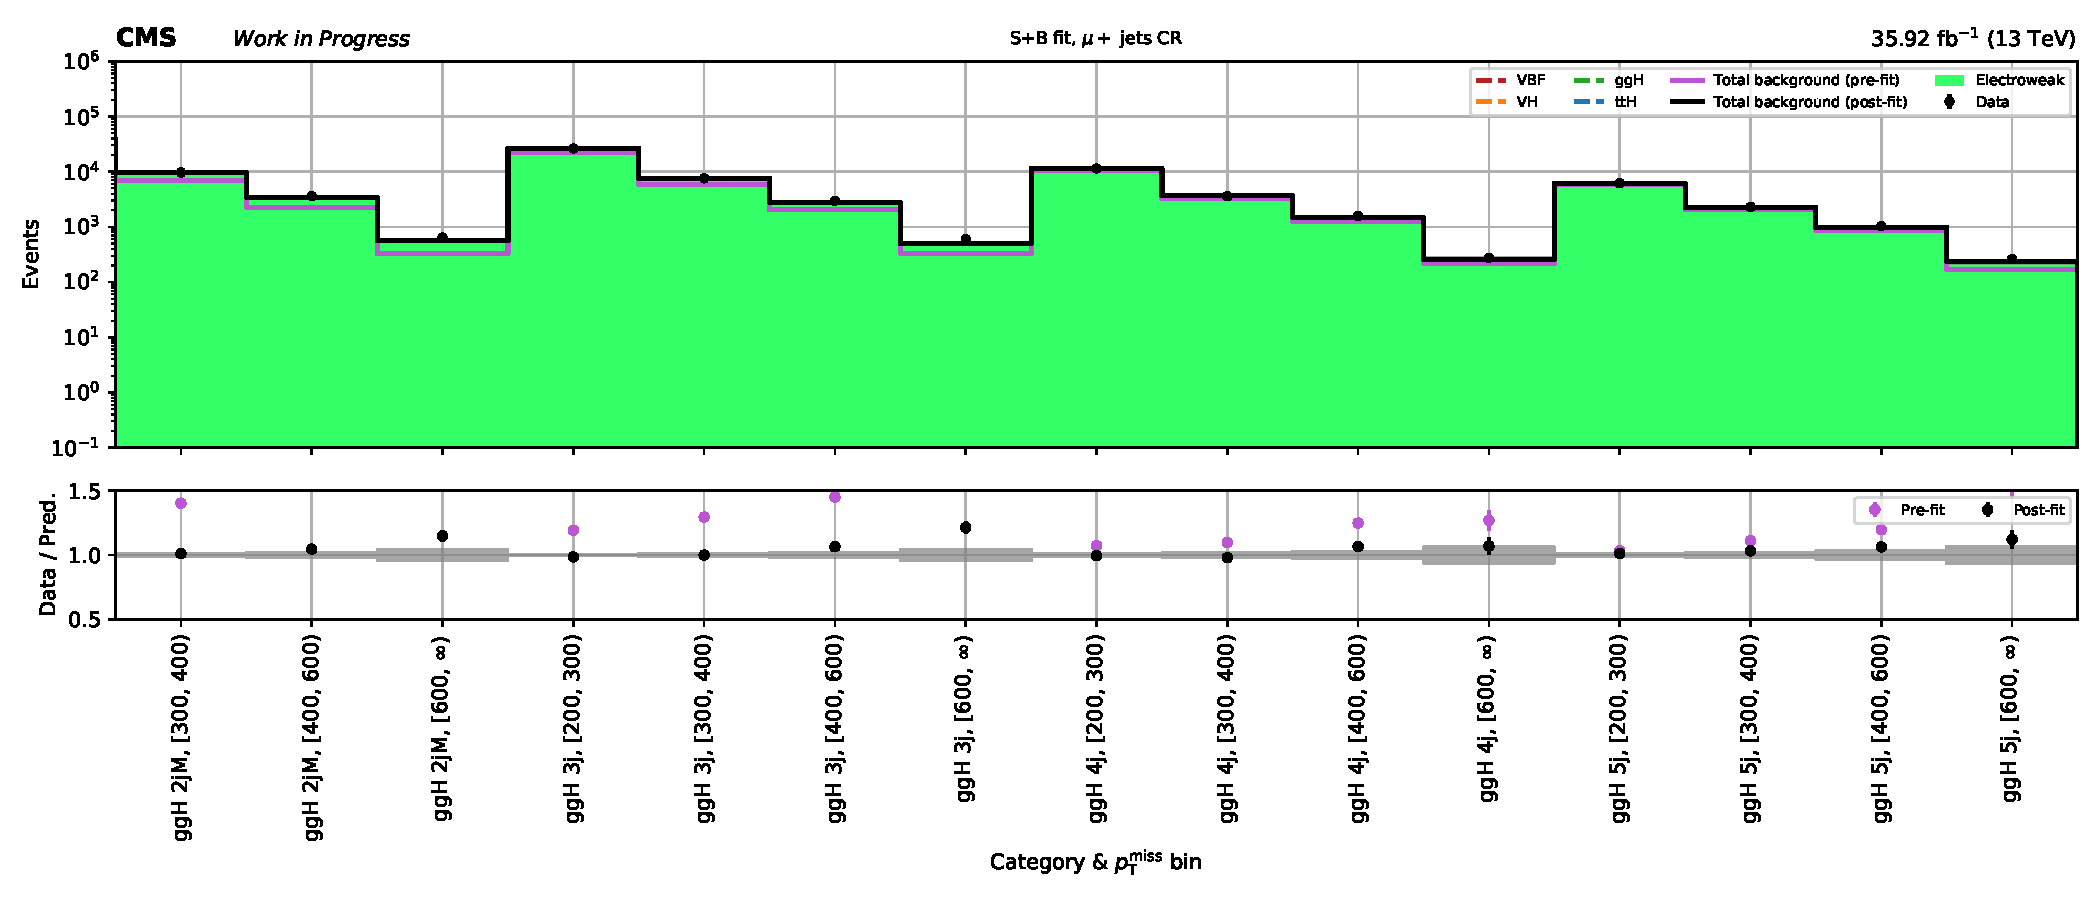
\includegraphics[width=\textwidth]{chapters/higgstoinv/figures/mountain_ranges/2016/ggF/Wmunu_tree_fit_s-abs_values_ggF_cats.pdf}
        \caption{\ggH --- \singleMuCr \gls{CR} (2016)}
    \end{subfigure}

    \begin{subfigure}[b]{0.66\textwidth}
        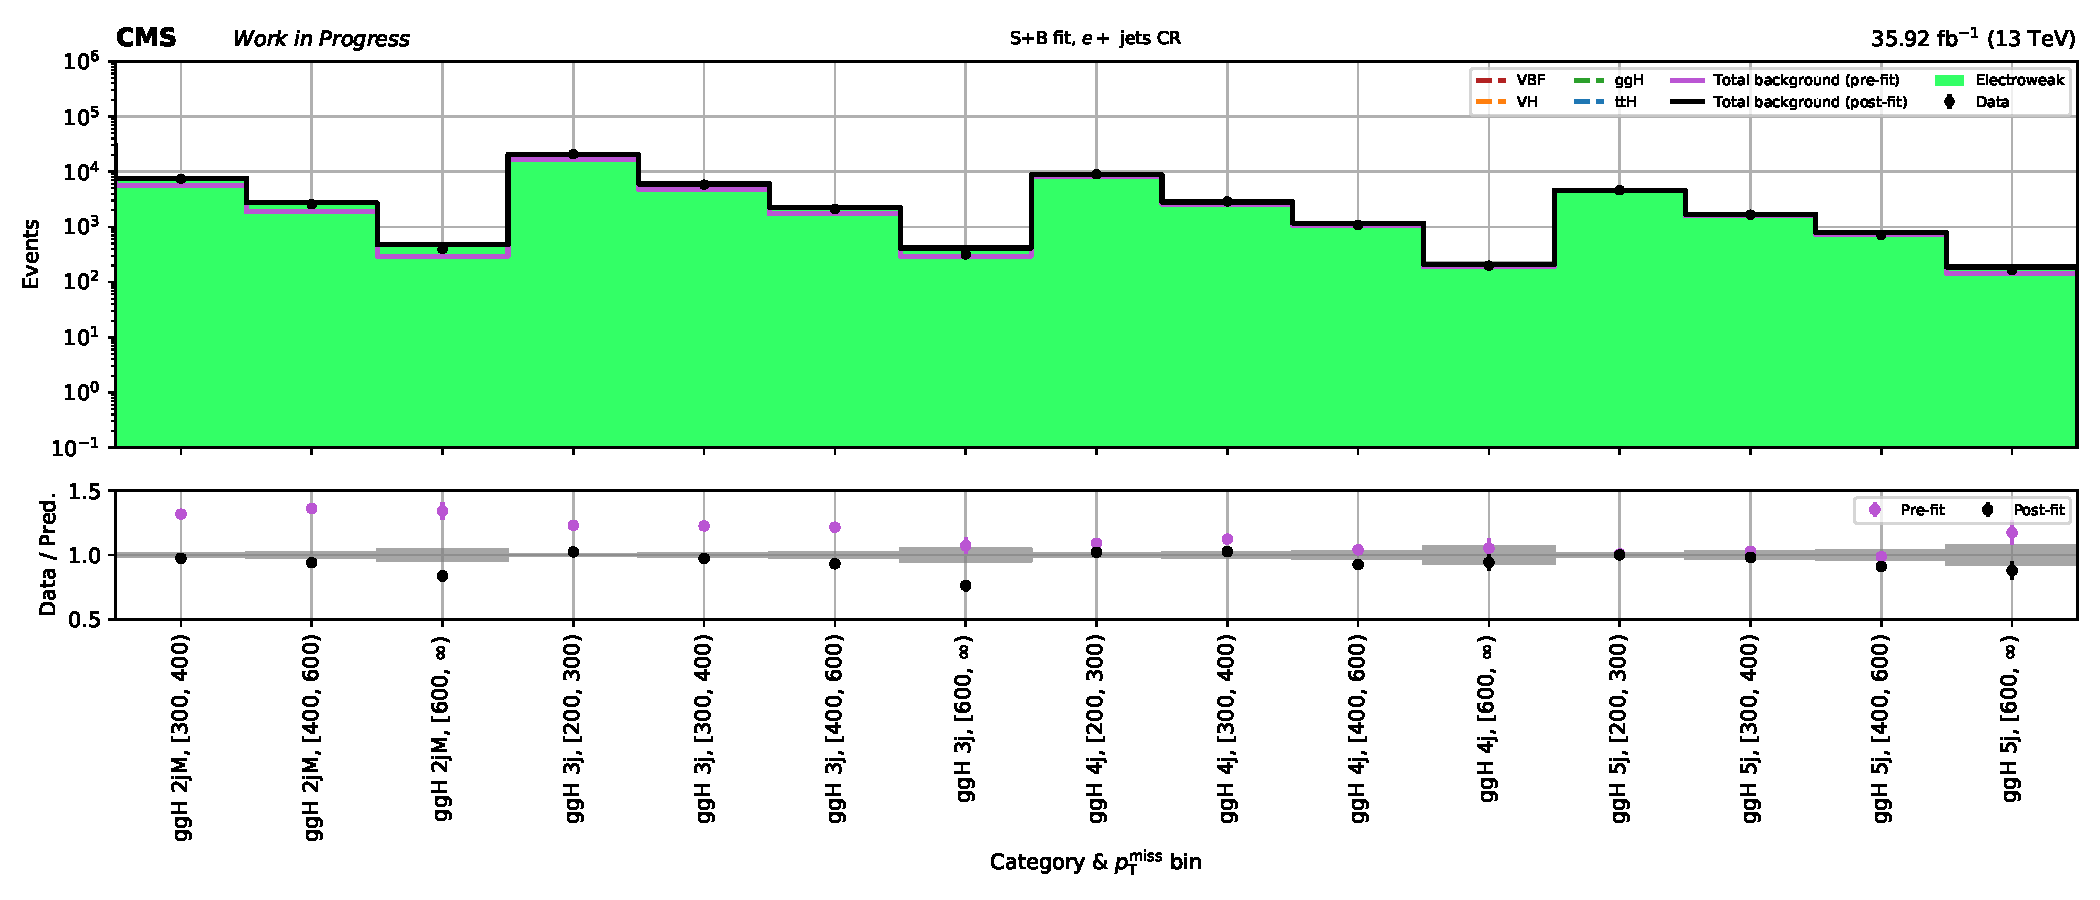
\includegraphics[width=\textwidth]{chapters/higgstoinv/figures/mountain_ranges/2016/ggF/Wenu_tree_fit_s-abs_values_ggF_cats.pdf}
        \caption{\ggH --- \singleEleCr \gls{CR} (2016)}
    \end{subfigure}

    \begin{subfigure}[b]{0.66\textwidth}
        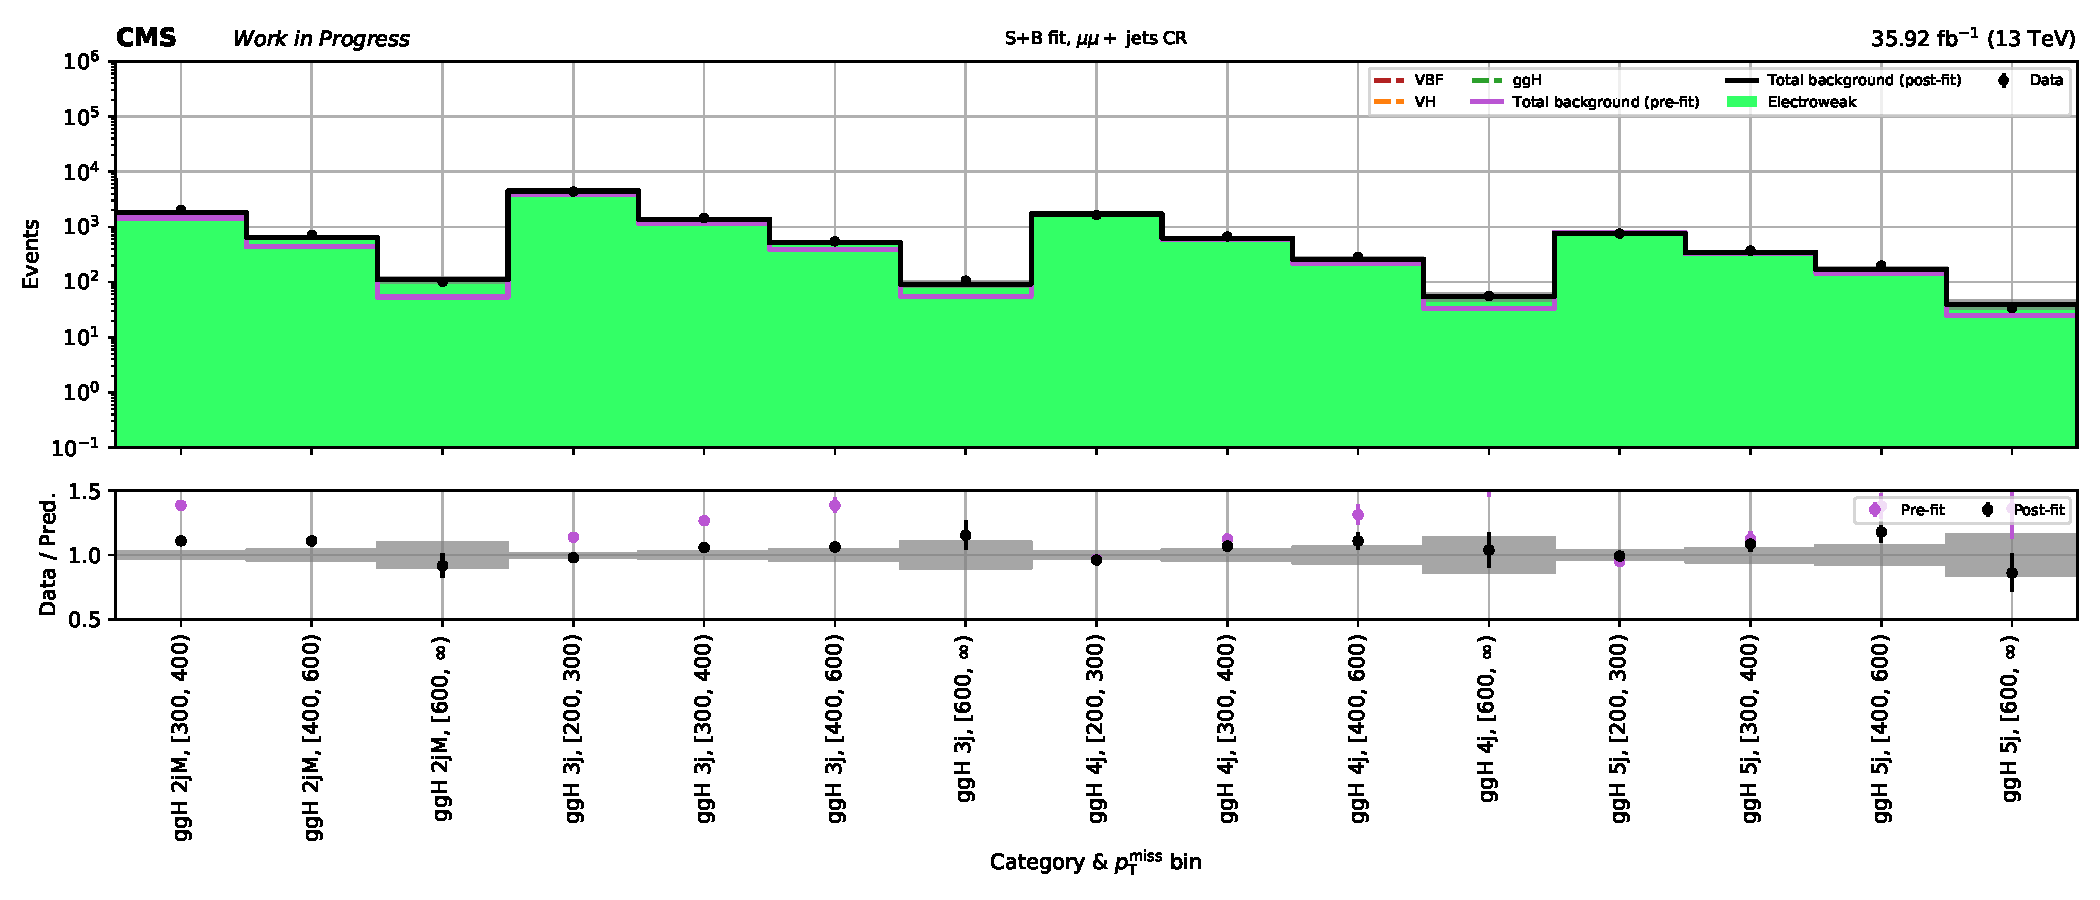
\includegraphics[width=\textwidth]{chapters/higgstoinv/figures/mountain_ranges/2016/ggF/Zmumu_tree_fit_s-abs_values_ggF_cats.pdf}
        \caption{\ggH --- \doubleMuCr \gls{CR} (2016)}
    \end{subfigure}

    \begin{subfigure}[b]{0.66\textwidth}
        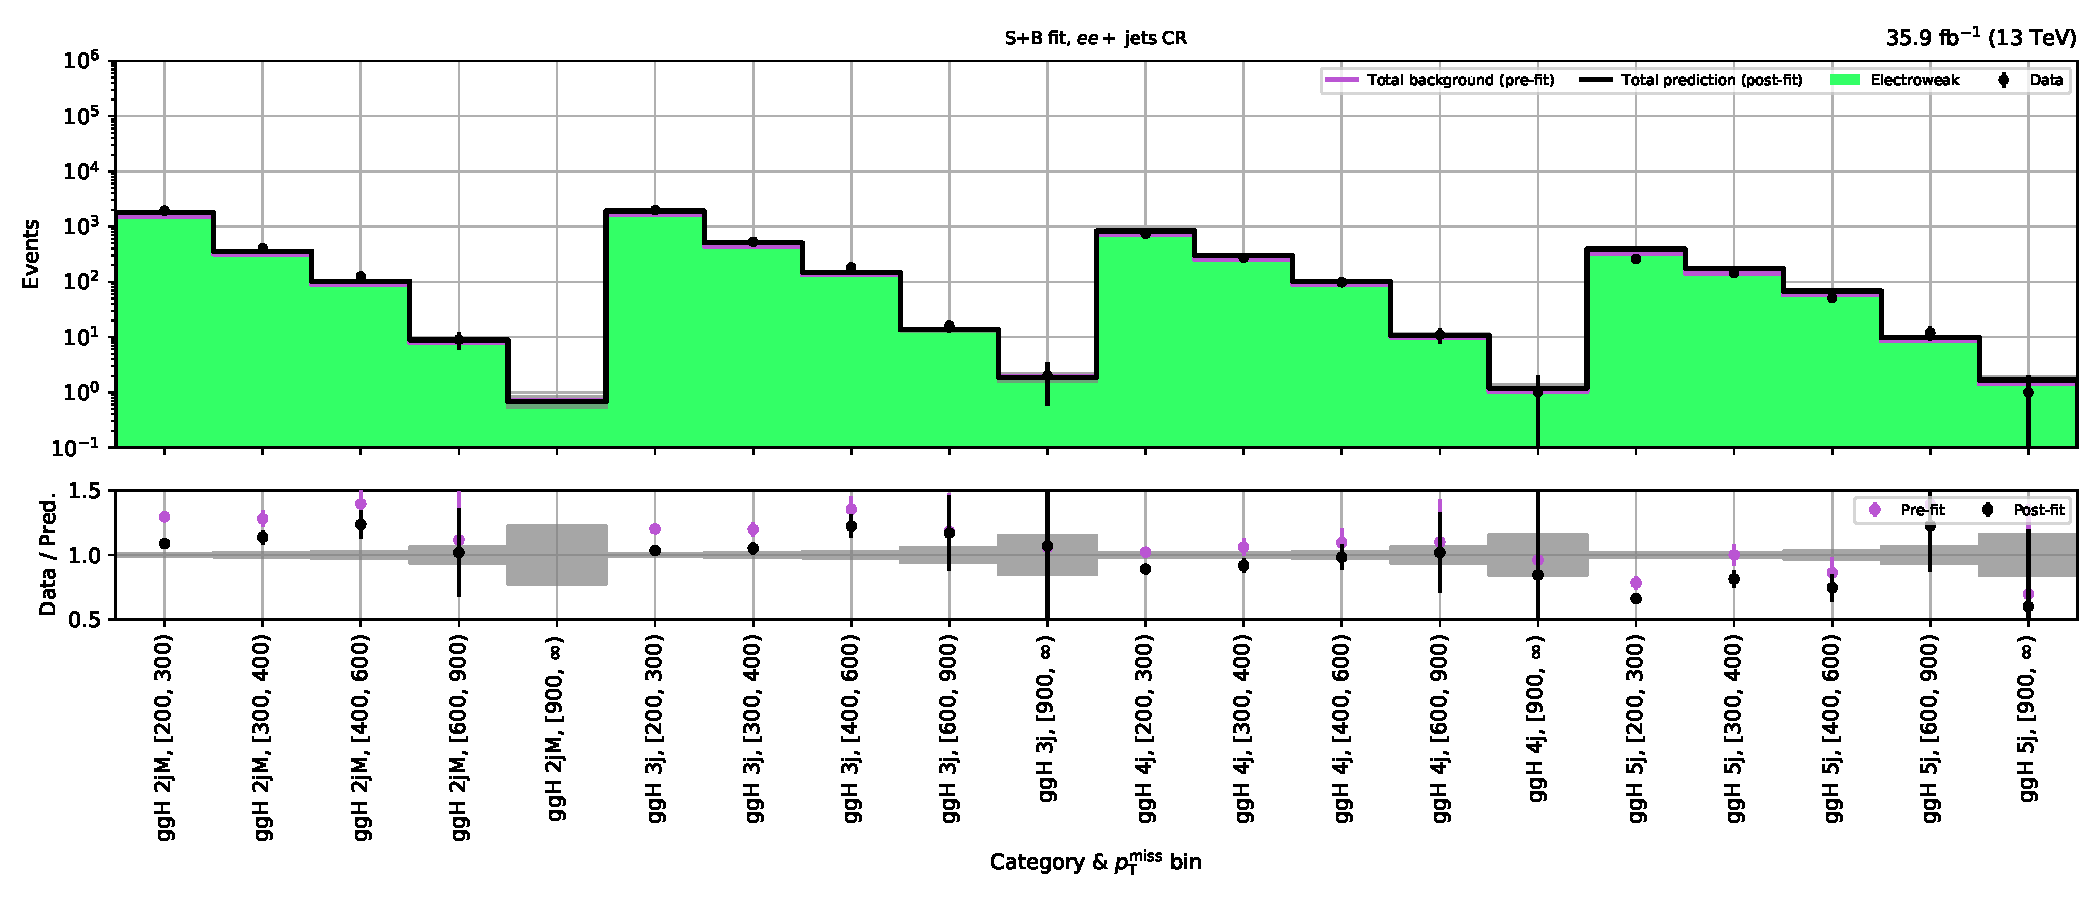
\includegraphics[width=\textwidth]{chapters/higgstoinv/figures/mountain_ranges/2016/ggF/Zee_tree_fit_s-abs_values_ggF_cats.pdf}
        \caption{\ggH --- \doubleEleCr \gls{CR} (2016)}
    \end{subfigure}

    \begin{subfigure}[b]{0.66\textwidth}
        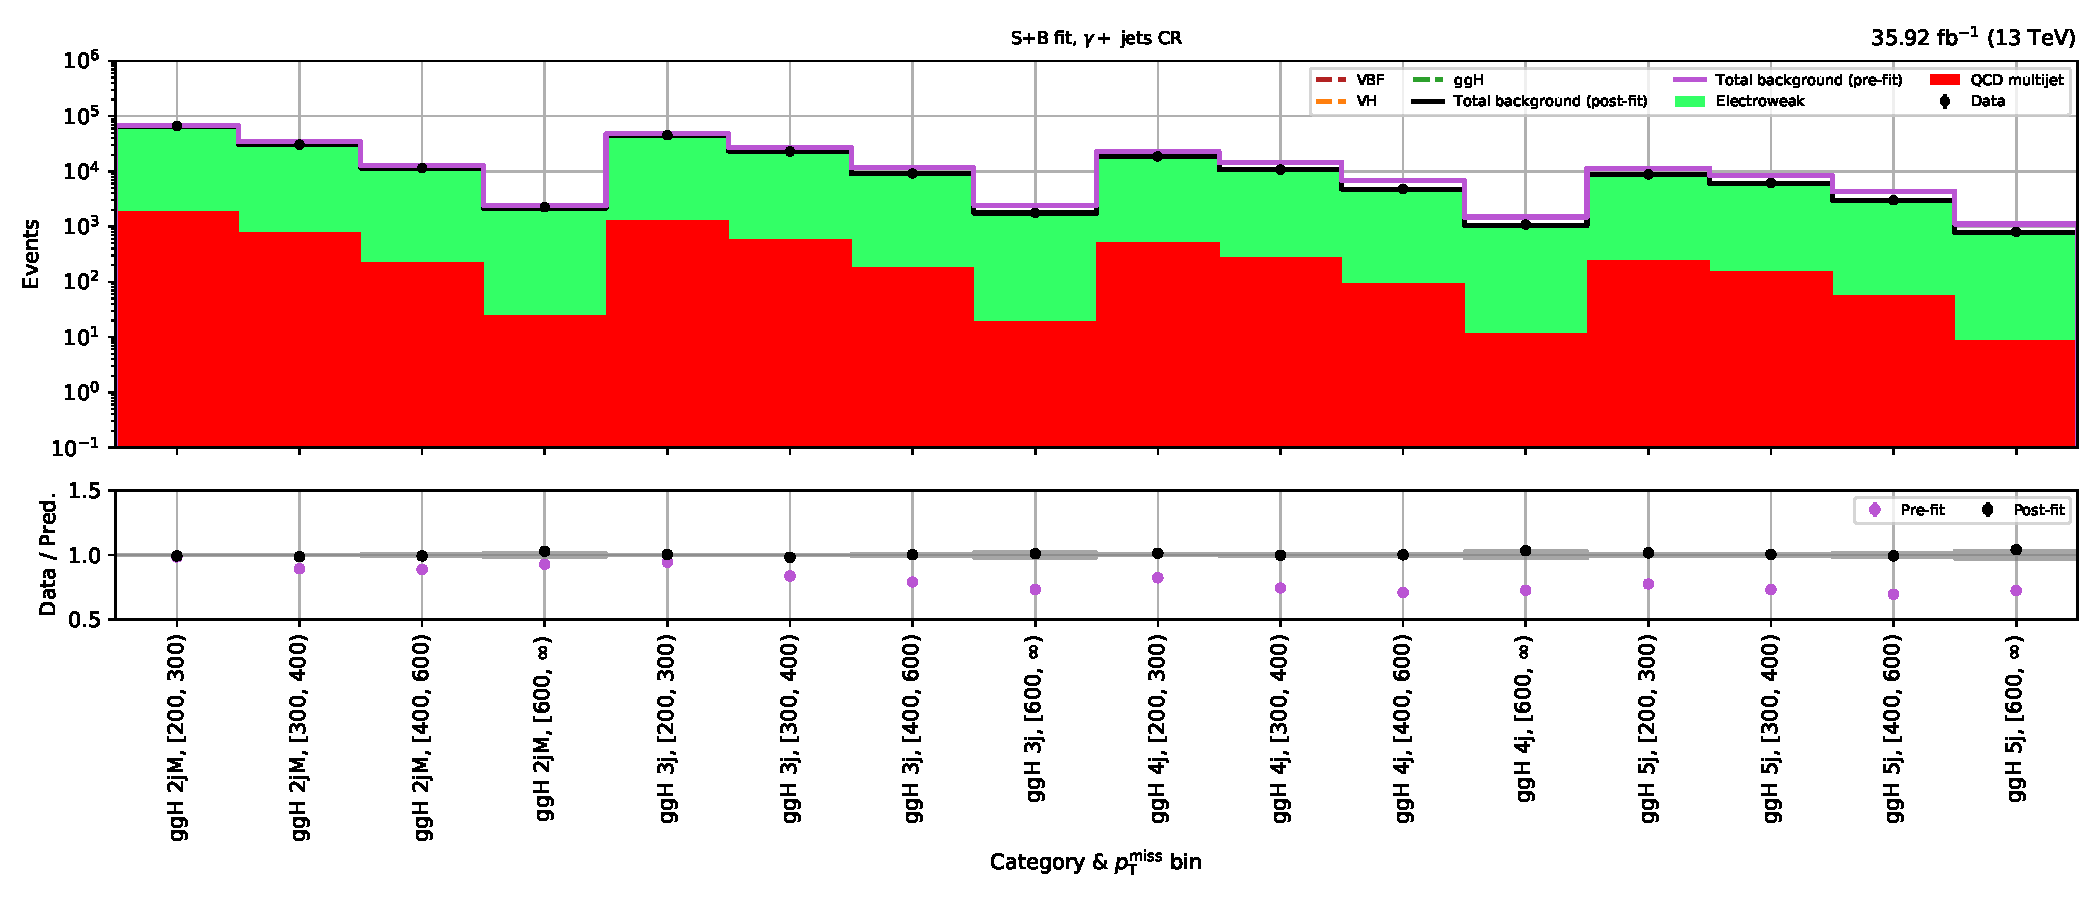
\includegraphics[width=\textwidth]{chapters/higgstoinv/figures/mountain_ranges/2016/ggF/Photon_tree_fit_s-abs_values_ggF_cats.pdf}
        \caption{\ggH --- \singlePhotonCr \gls{CR} (2016)}
    \end{subfigure}
    \caption[Post-fit yields for each \ggH subcategory and \ptmiss bin in the lepton and photon control regions for the 2016 dataset]{Post-fit yields for each \ggH subcategory and \ptmiss bin in the lepton and photon \glspl{CR} for the 2016 dataset. The total background pre-fit and post-fit is compared in the lower panel of each subfigure.}
    \label{fig:htoinv_mountain_range_ggF_2016_CRs}
\end{figure}

\begin{figure}[htbp]
    \centering
    \begin{subfigure}[b]{0.66\textwidth}
        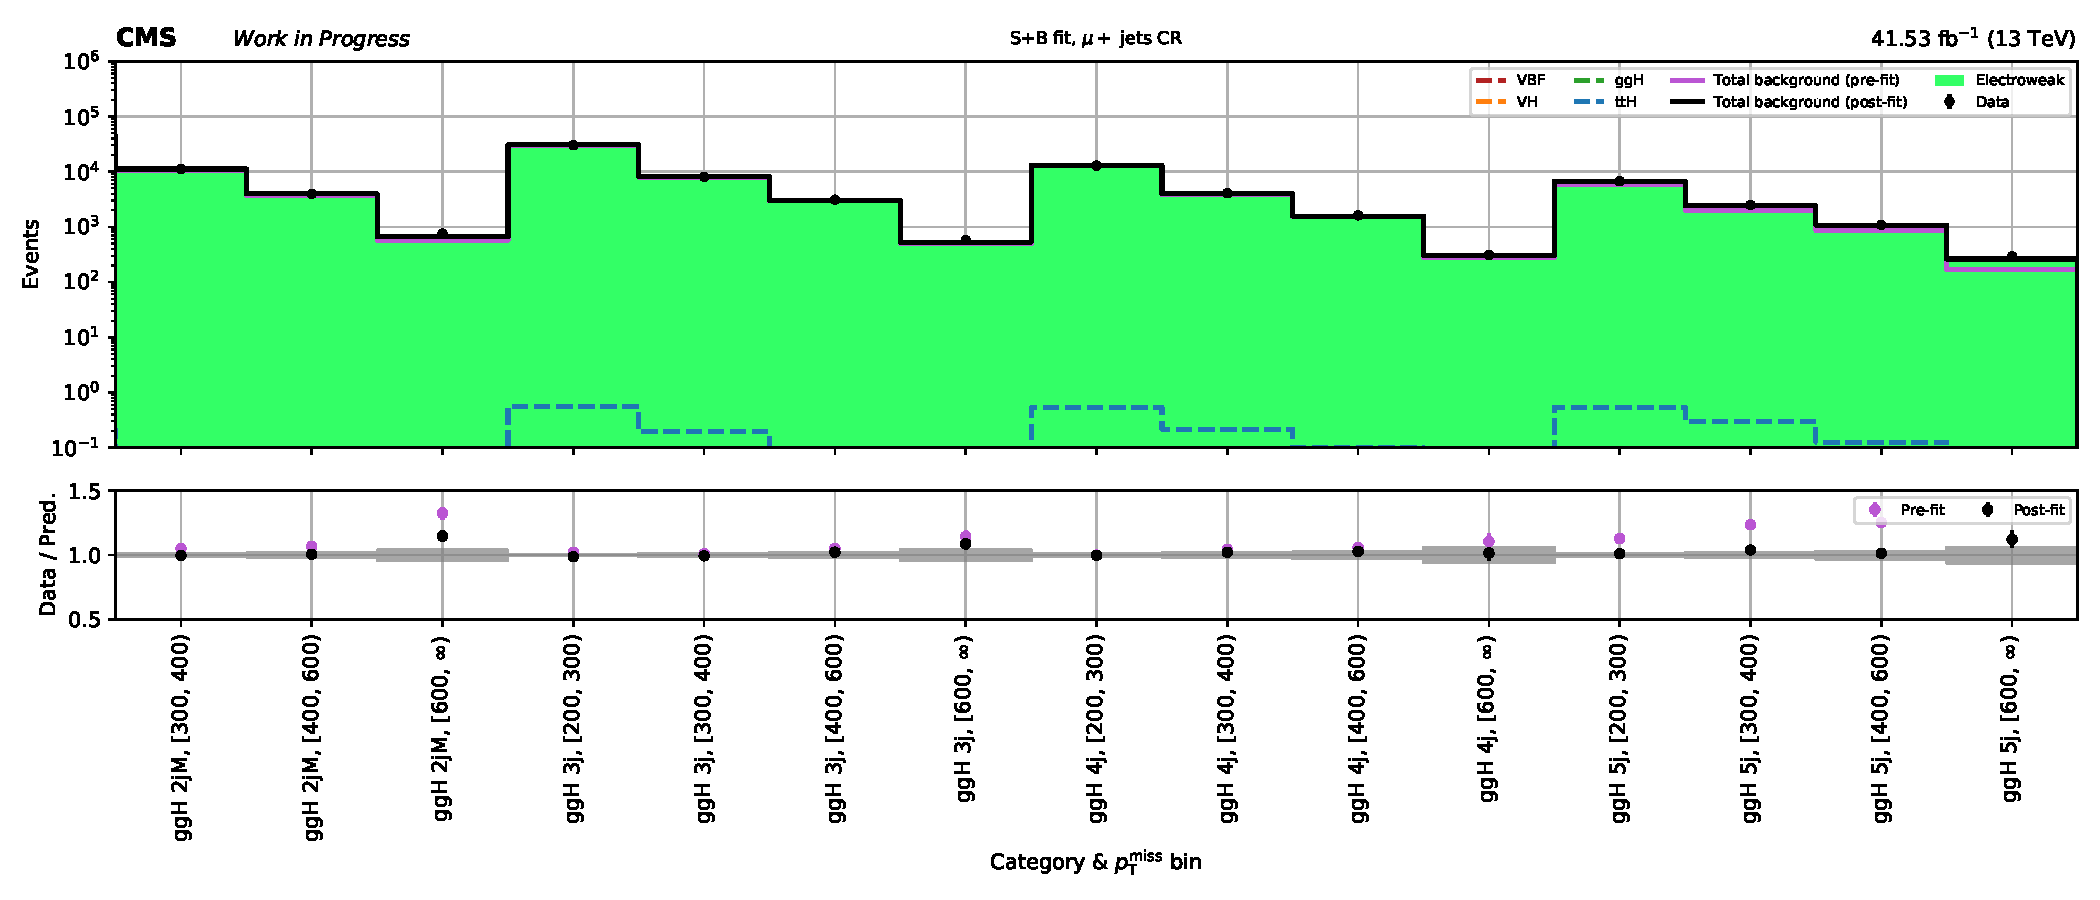
\includegraphics[width=\textwidth]{chapters/higgstoinv/figures/mountain_ranges/2017/ggF/Wmunu_tree_fit_s-abs_values_ggF_cats.pdf}
        \caption{\ggH --- \singleMuCr \gls{CR} (2017)}
    \end{subfigure}

    \begin{subfigure}[b]{0.66\textwidth}
        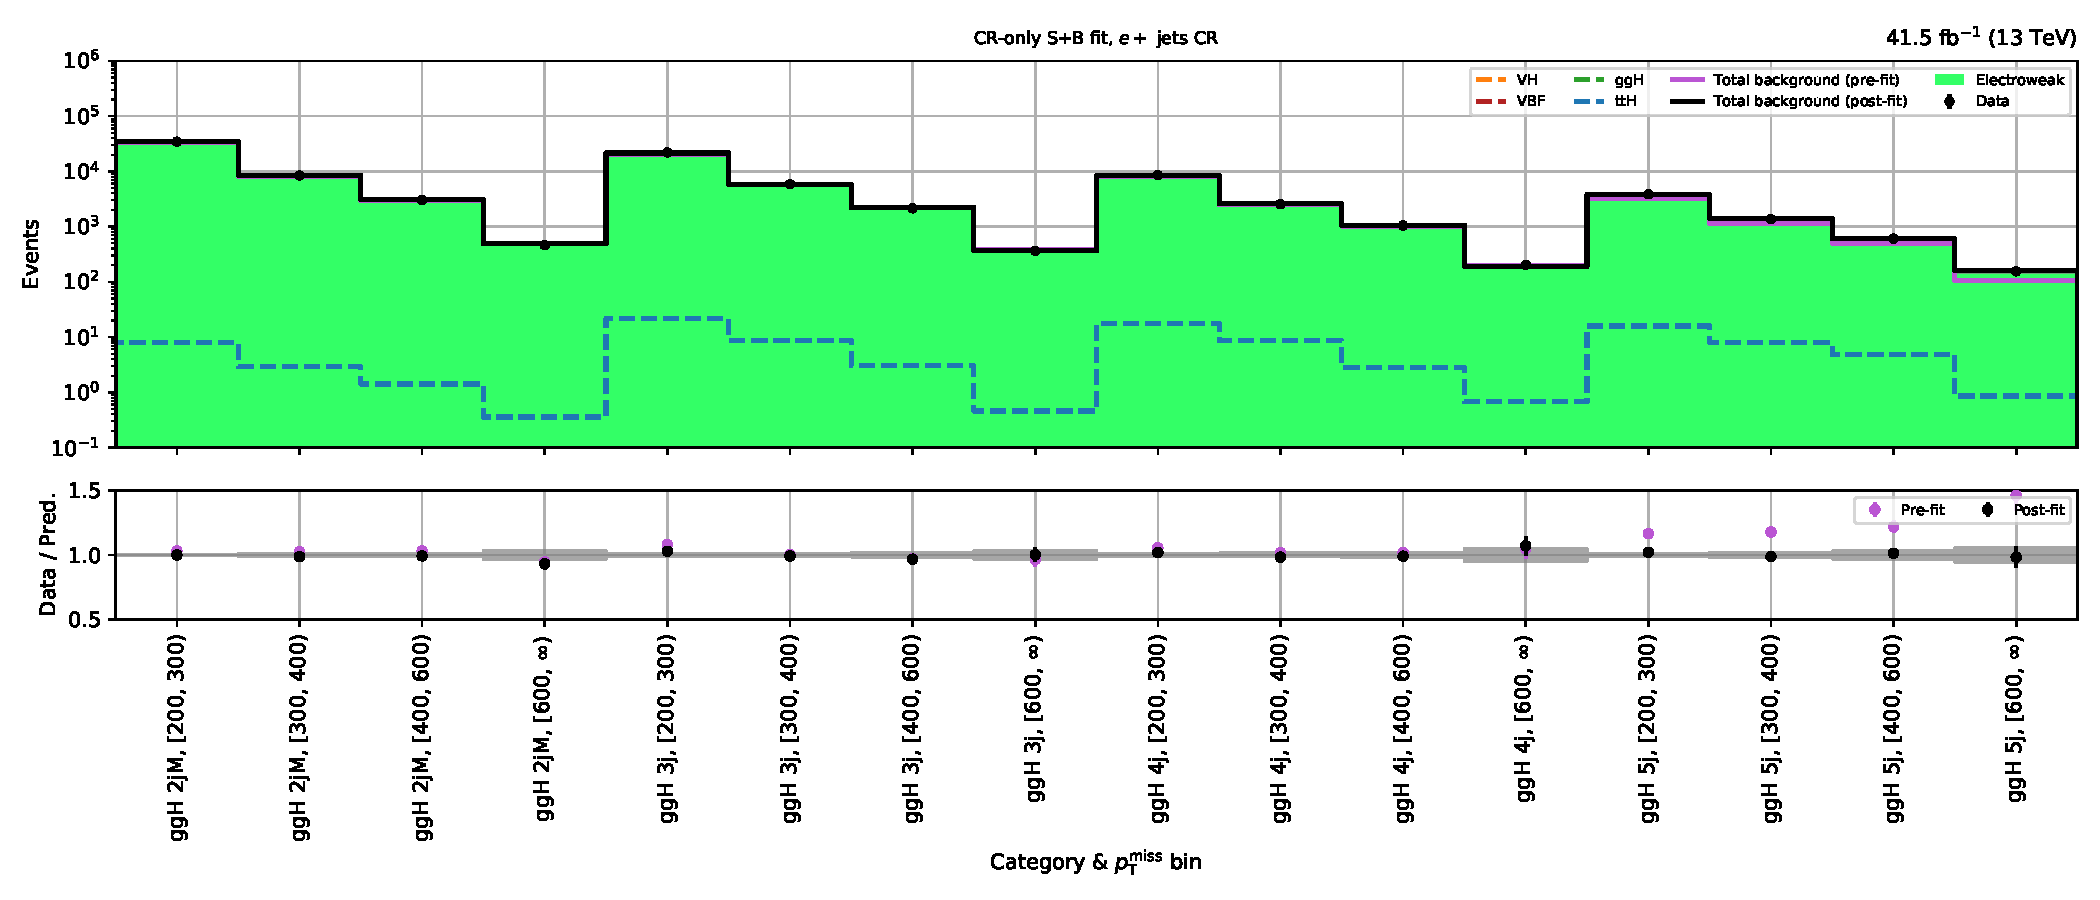
\includegraphics[width=\textwidth]{chapters/higgstoinv/figures/mountain_ranges/2017/ggF/Wenu_tree_fit_s-abs_values_ggF_cats.pdf}
        \caption{\ggH --- \singleEleCr \gls{CR} (2017)}
    \end{subfigure}

    \begin{subfigure}[b]{0.66\textwidth}
        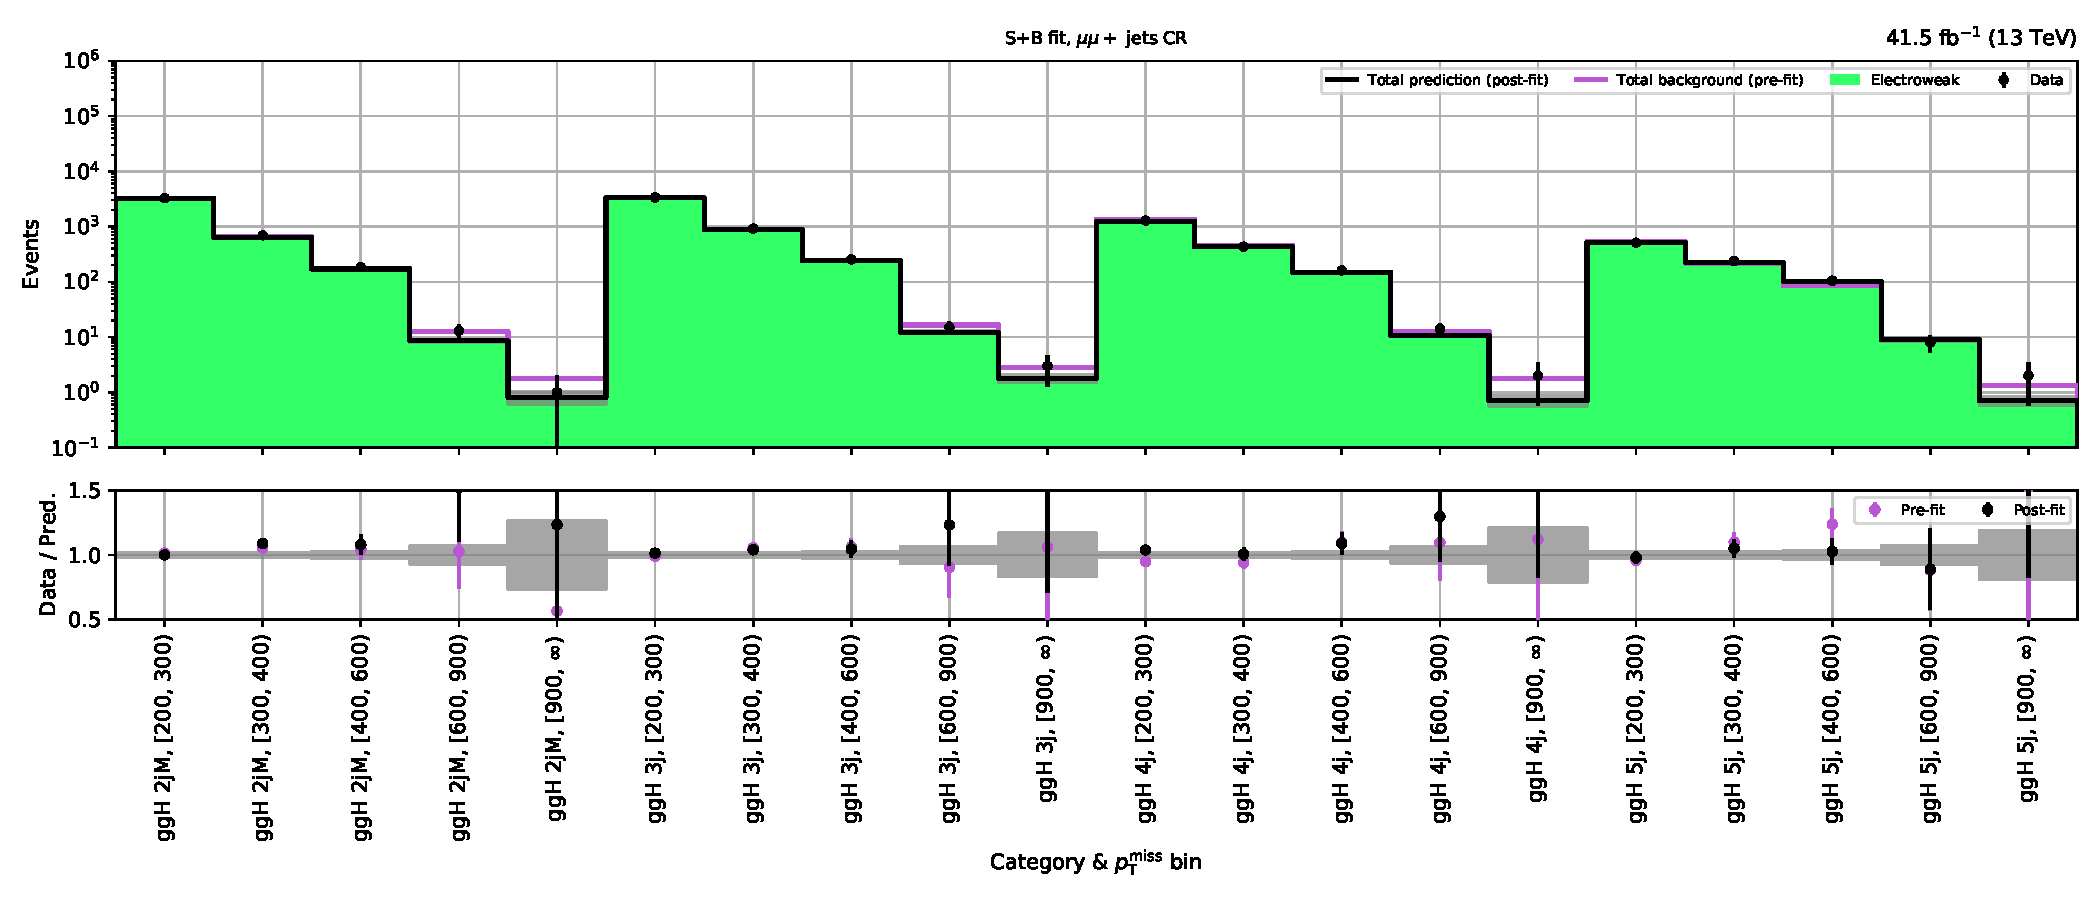
\includegraphics[width=\textwidth]{chapters/higgstoinv/figures/mountain_ranges/2017/ggF/Zmumu_tree_fit_s-abs_values_ggF_cats.pdf}
        \caption{\ggH --- \doubleMuCr \gls{CR} (2017)}
    \end{subfigure}

    \begin{subfigure}[b]{0.66\textwidth}
        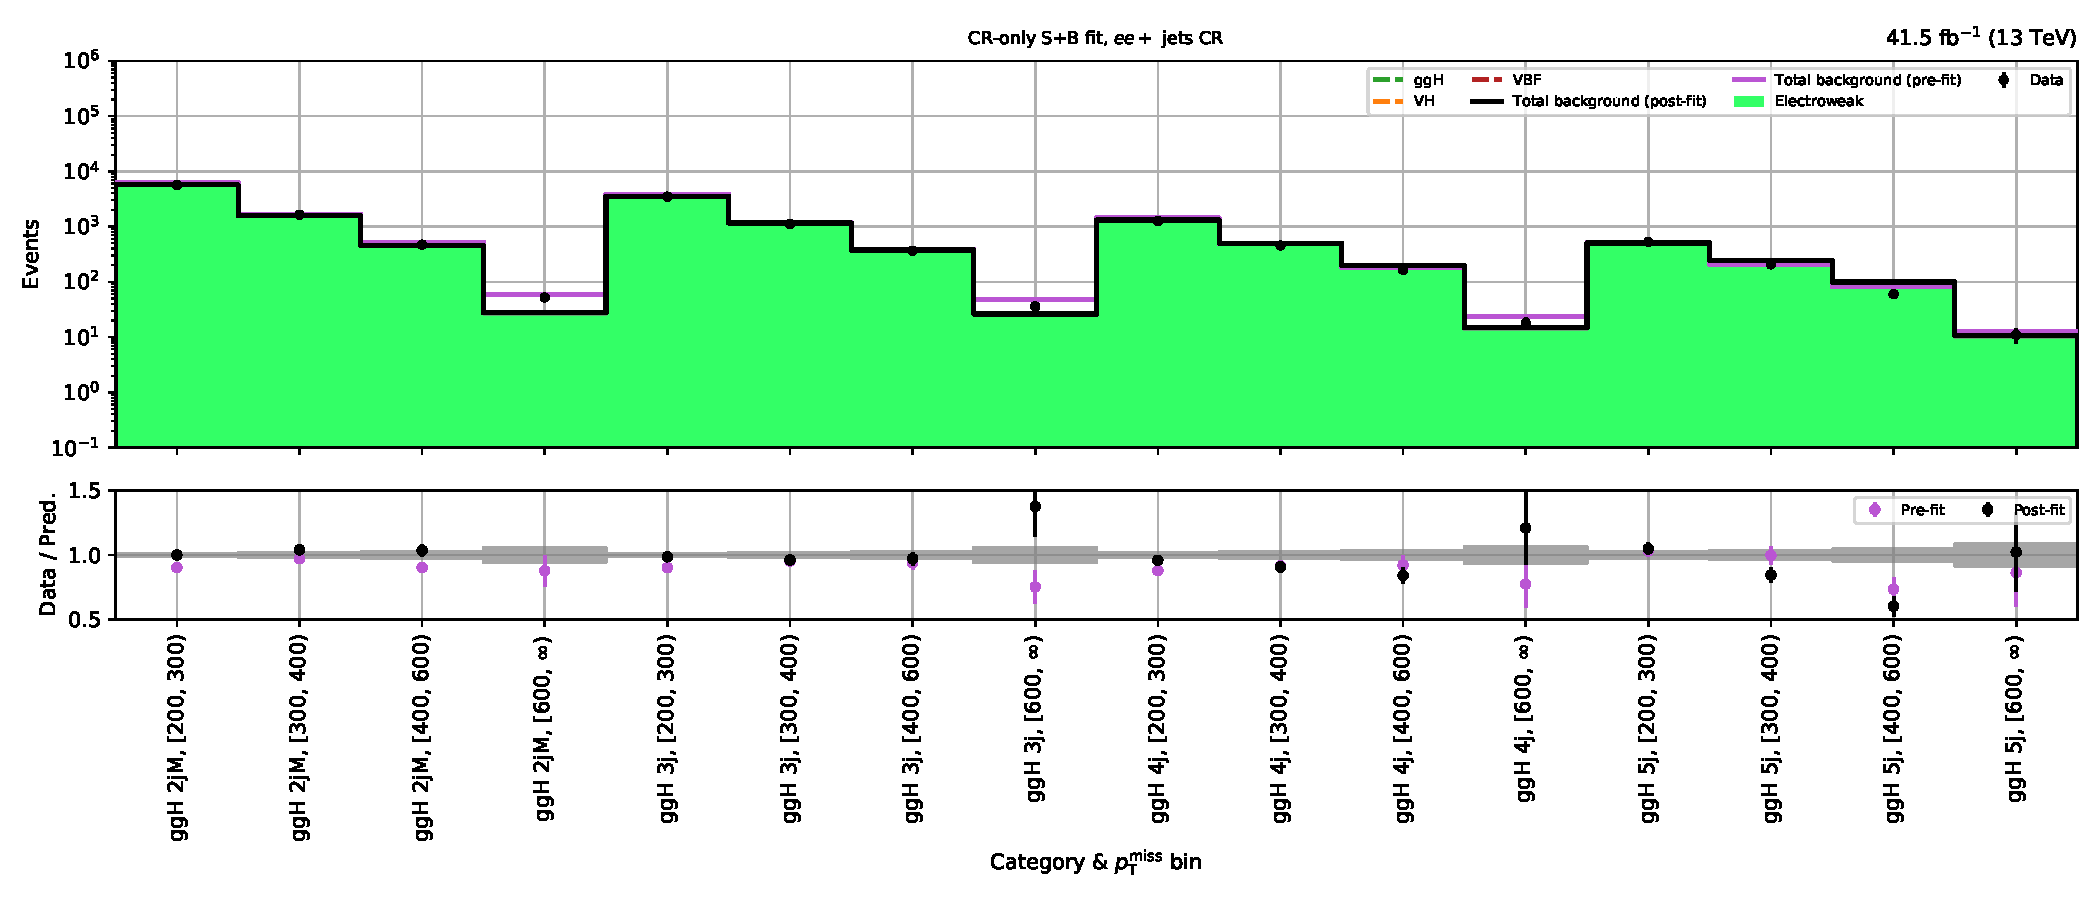
\includegraphics[width=\textwidth]{chapters/higgstoinv/figures/mountain_ranges/2017/ggF/Zee_tree_fit_s-abs_values_ggF_cats.pdf}
        \caption{\ggH --- \doubleEleCr \gls{CR} (2017)}
    \end{subfigure}

    \begin{subfigure}[b]{0.66\textwidth}
        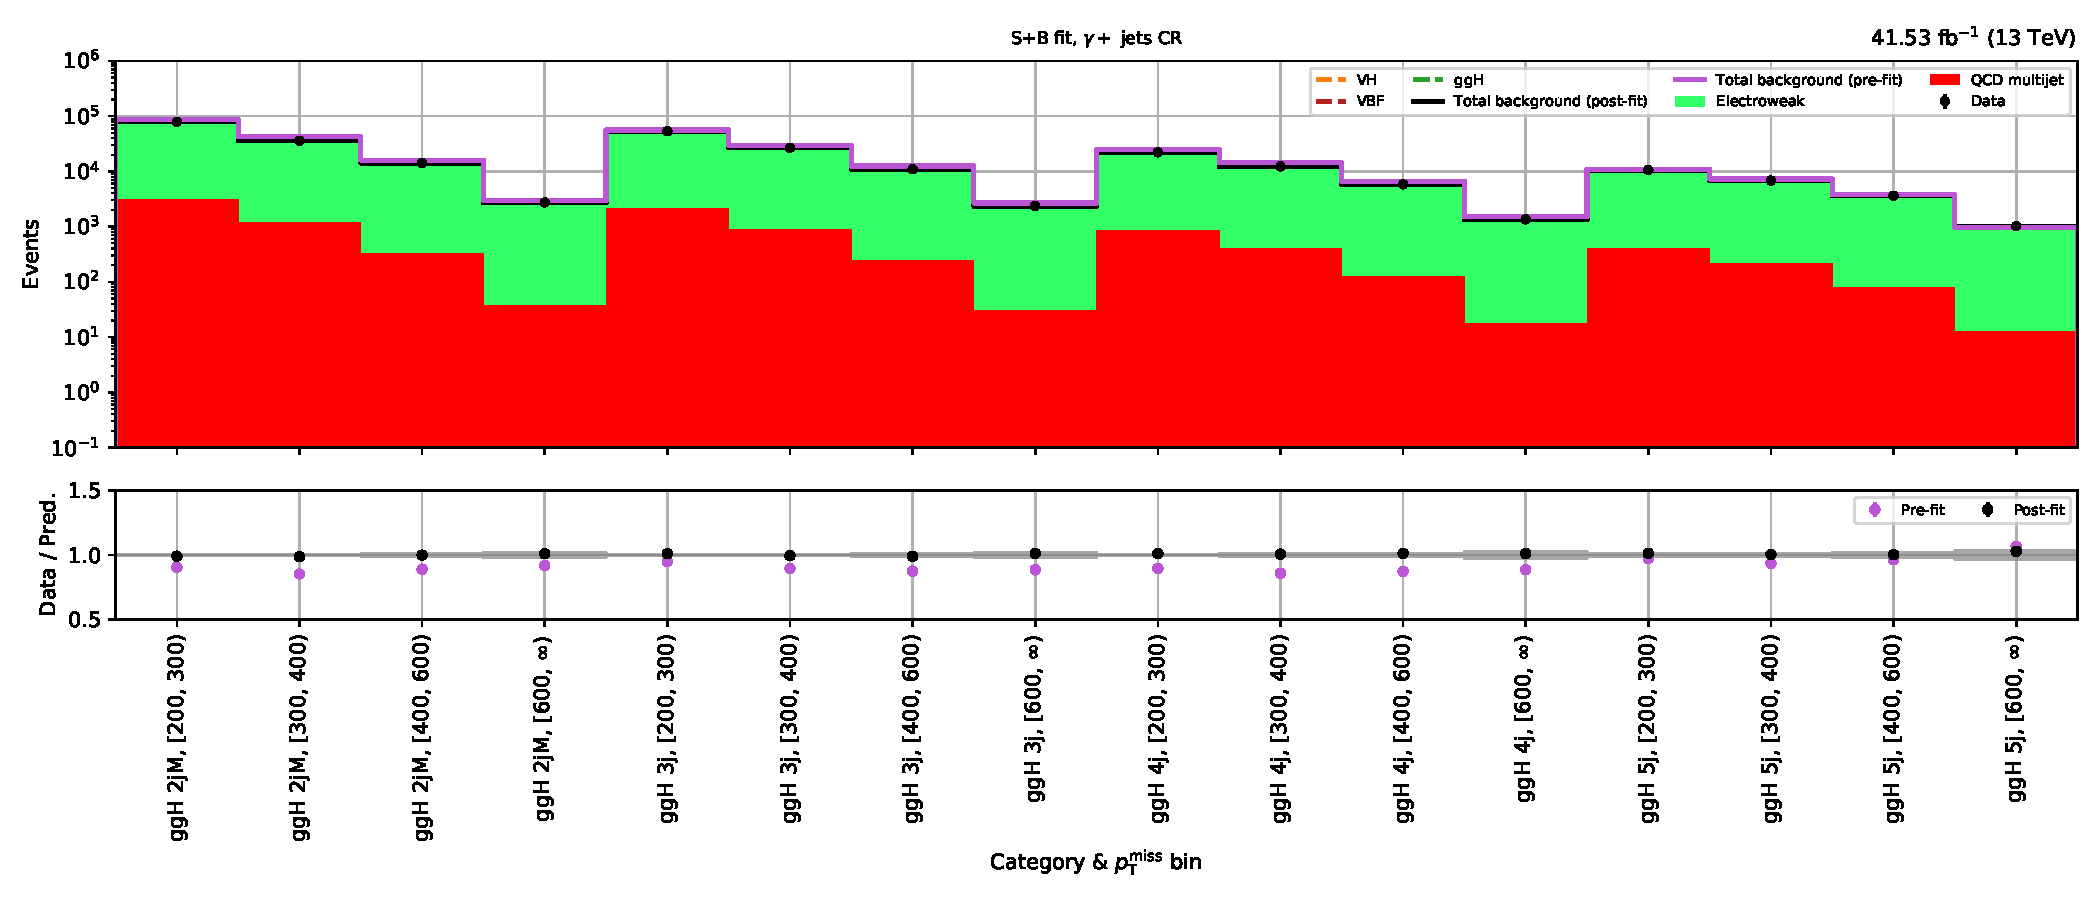
\includegraphics[width=\textwidth]{chapters/higgstoinv/figures/mountain_ranges/2017/ggF/Photon_tree_fit_s-abs_values_ggF_cats.pdf}
        \caption{\ggH --- \singlePhotonCr \gls{CR} (2017)}
    \end{subfigure}
    \caption[Post-fit yields for each \ggH subcategory and \ptmiss bin in the lepton and photon control regions for the 2017 dataset]{Post-fit yields for each \ggH subcategory and \ptmiss bin in the lepton and photon \glspl{CR} for the 2017 dataset. The total background pre-fit and post-fit is compared in the lower panel of each subfigure.}
    \label{fig:htoinv_mountain_range_ggF_2017_CRs}
\end{figure}

\begin{figure}[htbp]
    \centering
    \begin{subfigure}[b]{0.66\textwidth}
        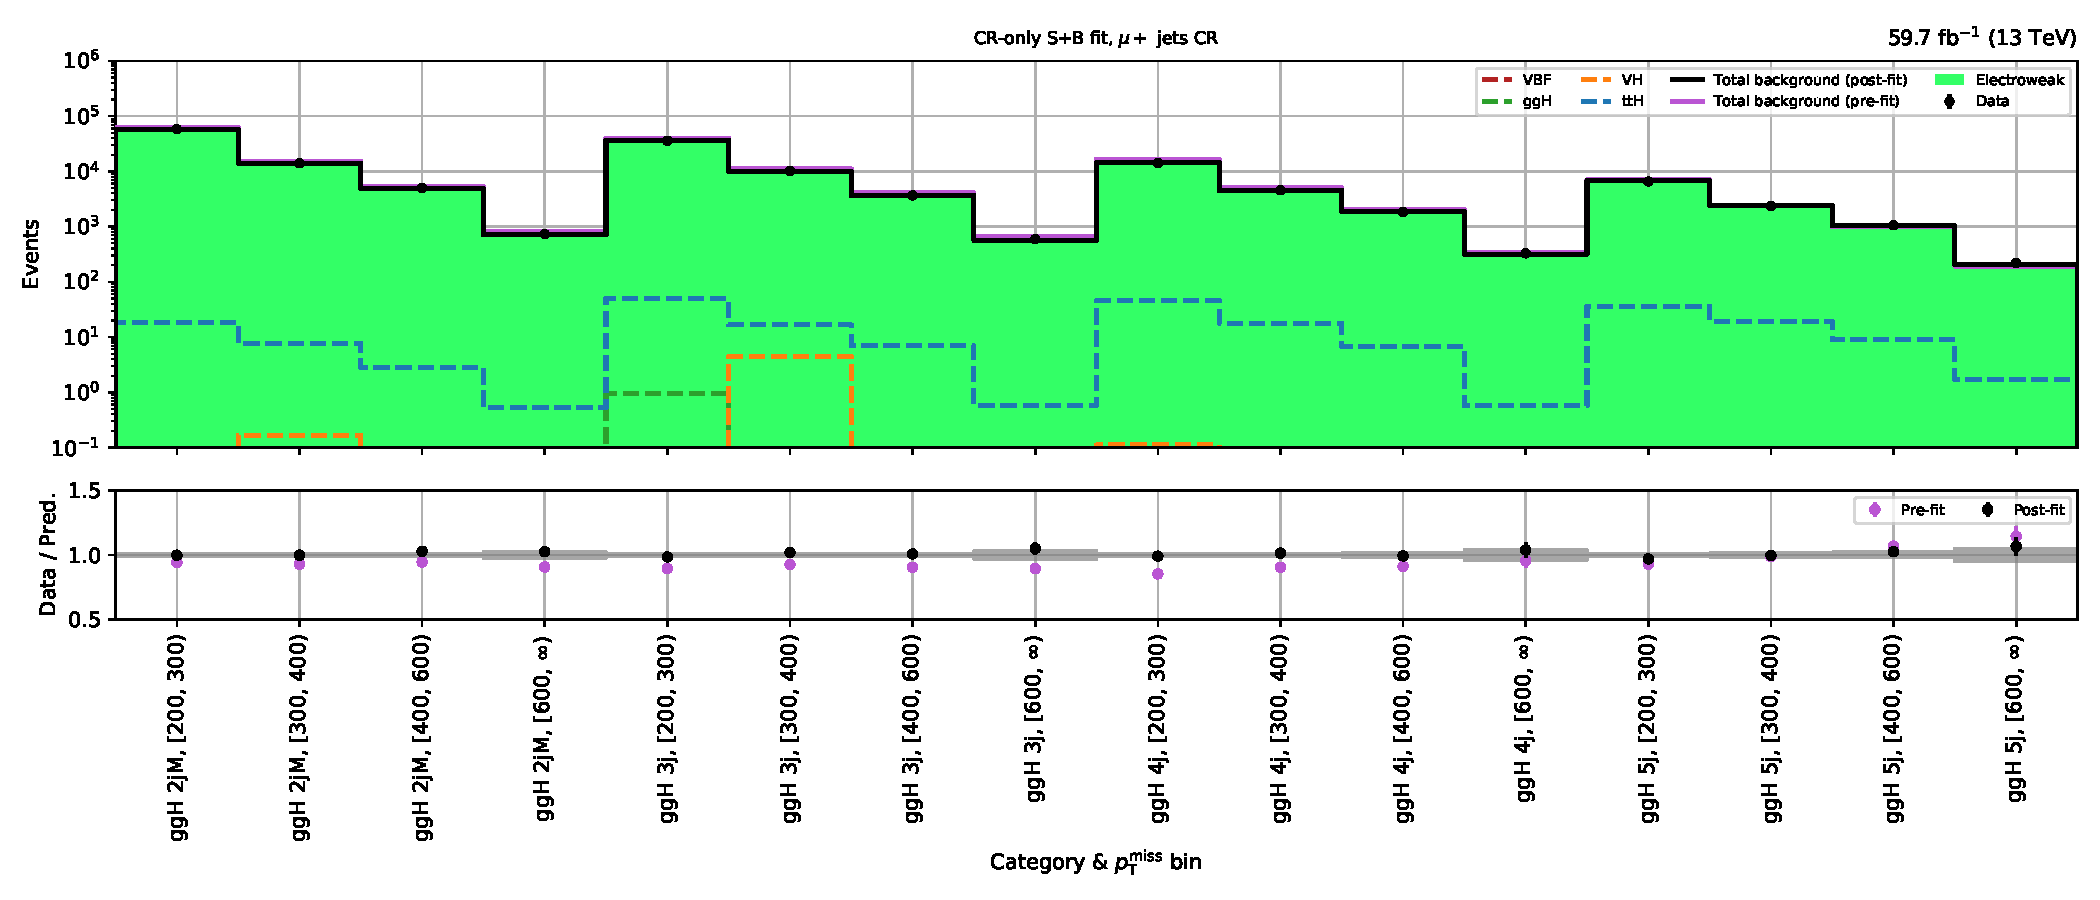
\includegraphics[width=\textwidth]{chapters/higgstoinv/figures/mountain_ranges/2018/ggF/Wmunu_tree_fit_s-abs_values_ggF_cats.pdf}
        \caption{\ggH --- \singleMuCr \gls{CR} (2018)}
    \end{subfigure}

    \begin{subfigure}[b]{0.66\textwidth}
        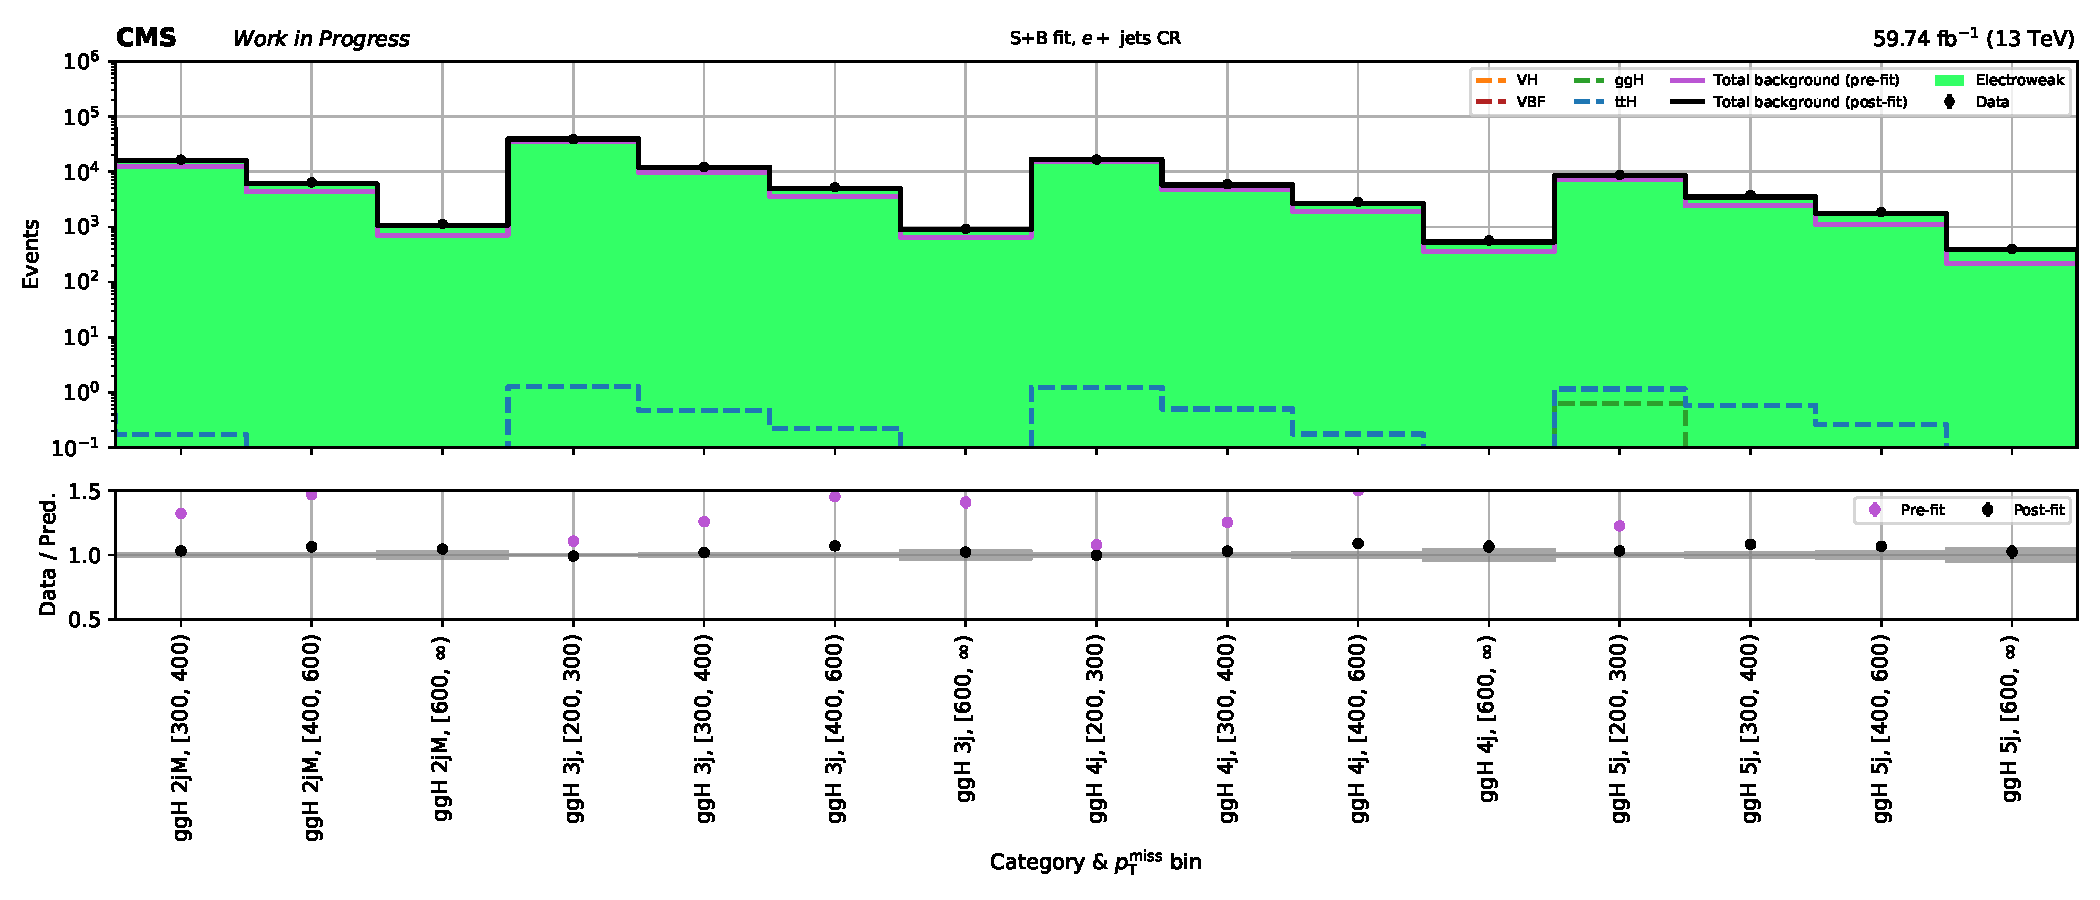
\includegraphics[width=\textwidth]{chapters/higgstoinv/figures/mountain_ranges/2018/ggF/Wenu_tree_fit_s-abs_values_ggF_cats.pdf}
        \caption{\ggH --- \singleEleCr \gls{CR} (2018)}
    \end{subfigure}

    \begin{subfigure}[b]{0.66\textwidth}
        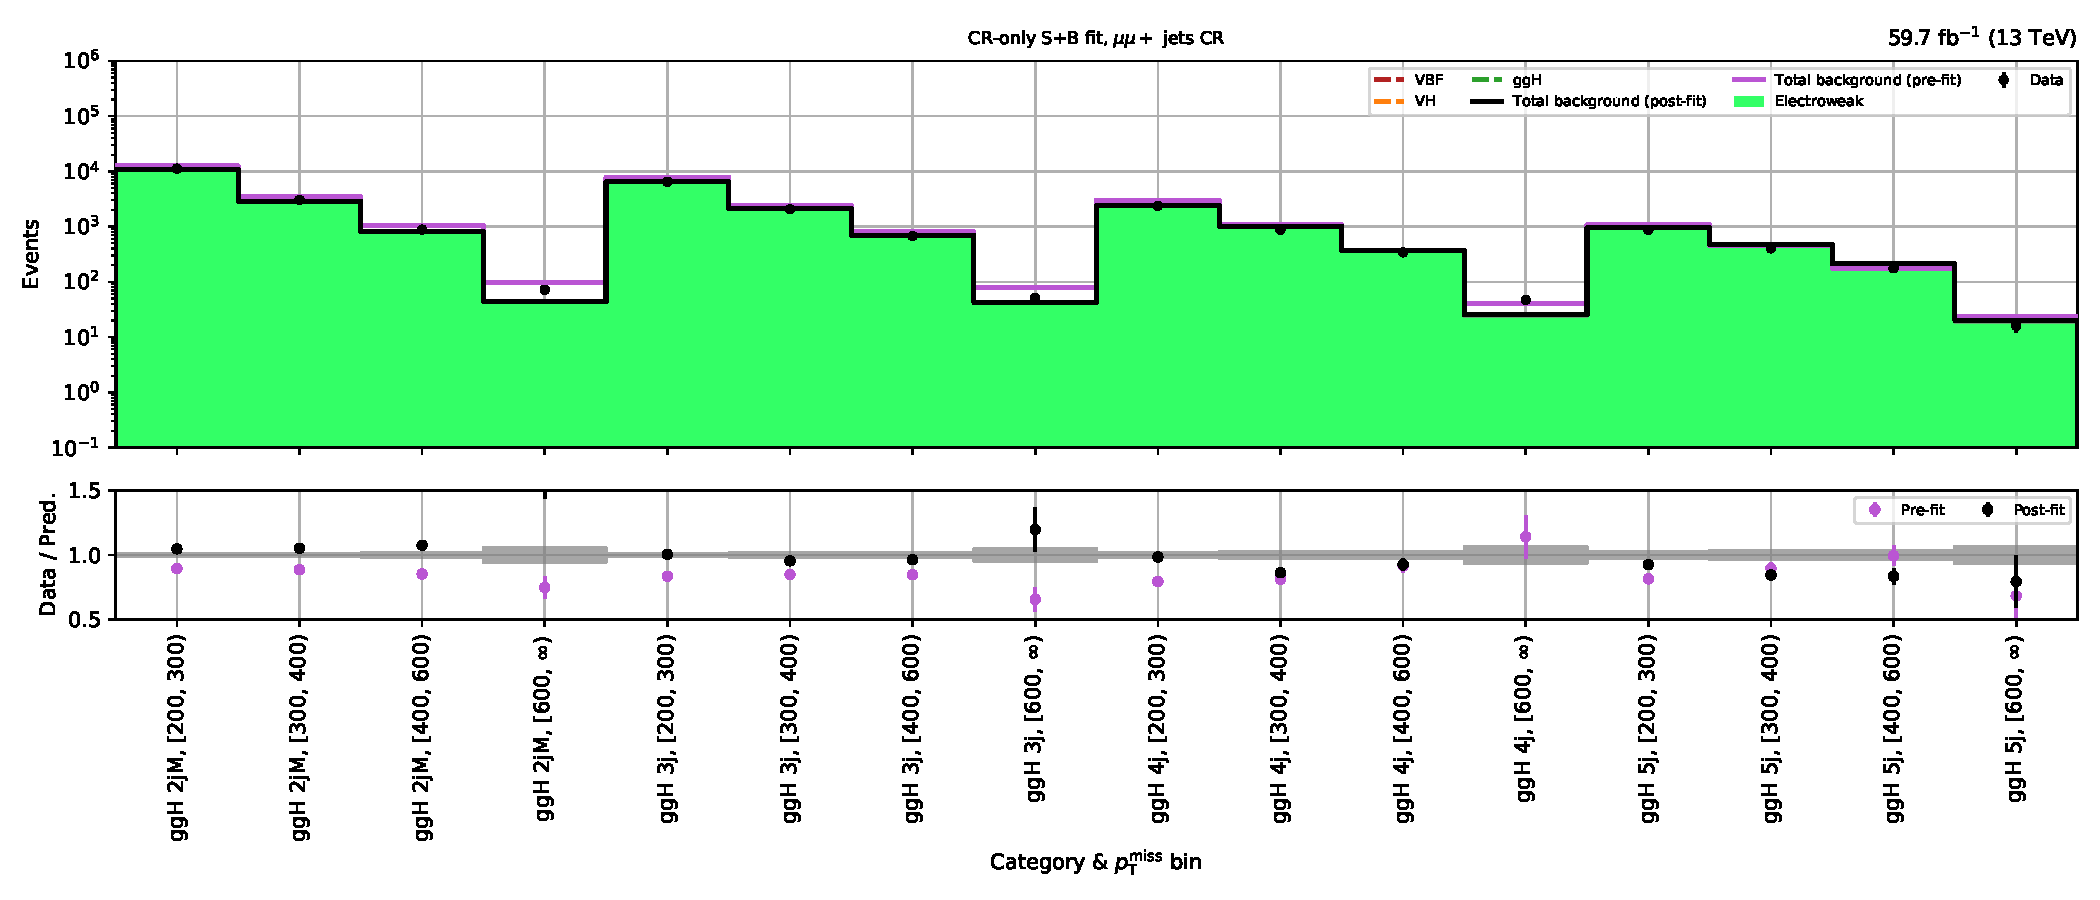
\includegraphics[width=\textwidth]{chapters/higgstoinv/figures/mountain_ranges/2018/ggF/Zmumu_tree_fit_s-abs_values_ggF_cats.pdf}
        \caption{\ggH --- \doubleMuCr \gls{CR} (2018)}
    \end{subfigure}

    \begin{subfigure}[b]{0.66\textwidth}
        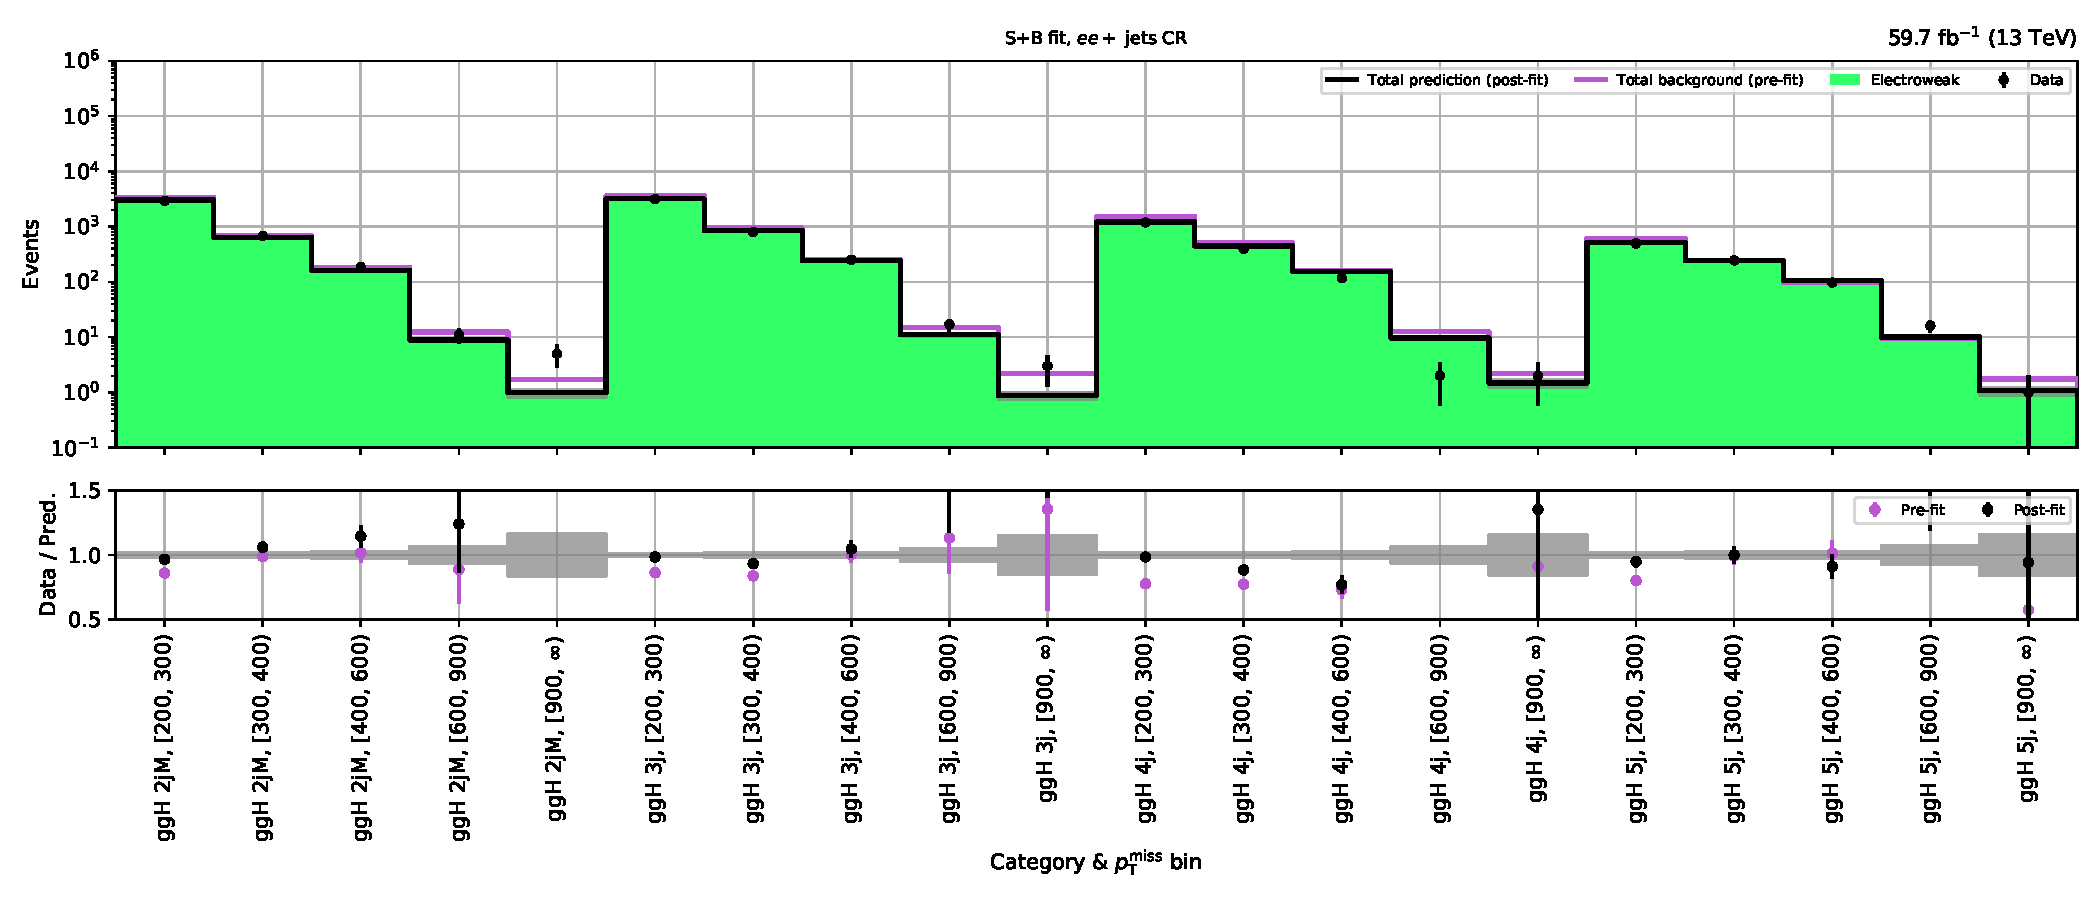
\includegraphics[width=\textwidth]{chapters/higgstoinv/figures/mountain_ranges/2018/ggF/Zee_tree_fit_s-abs_values_ggF_cats.pdf}
        \caption{\ggH --- \doubleEleCr \gls{CR} (2018)}
    \end{subfigure}

    \begin{subfigure}[b]{0.66\textwidth}
        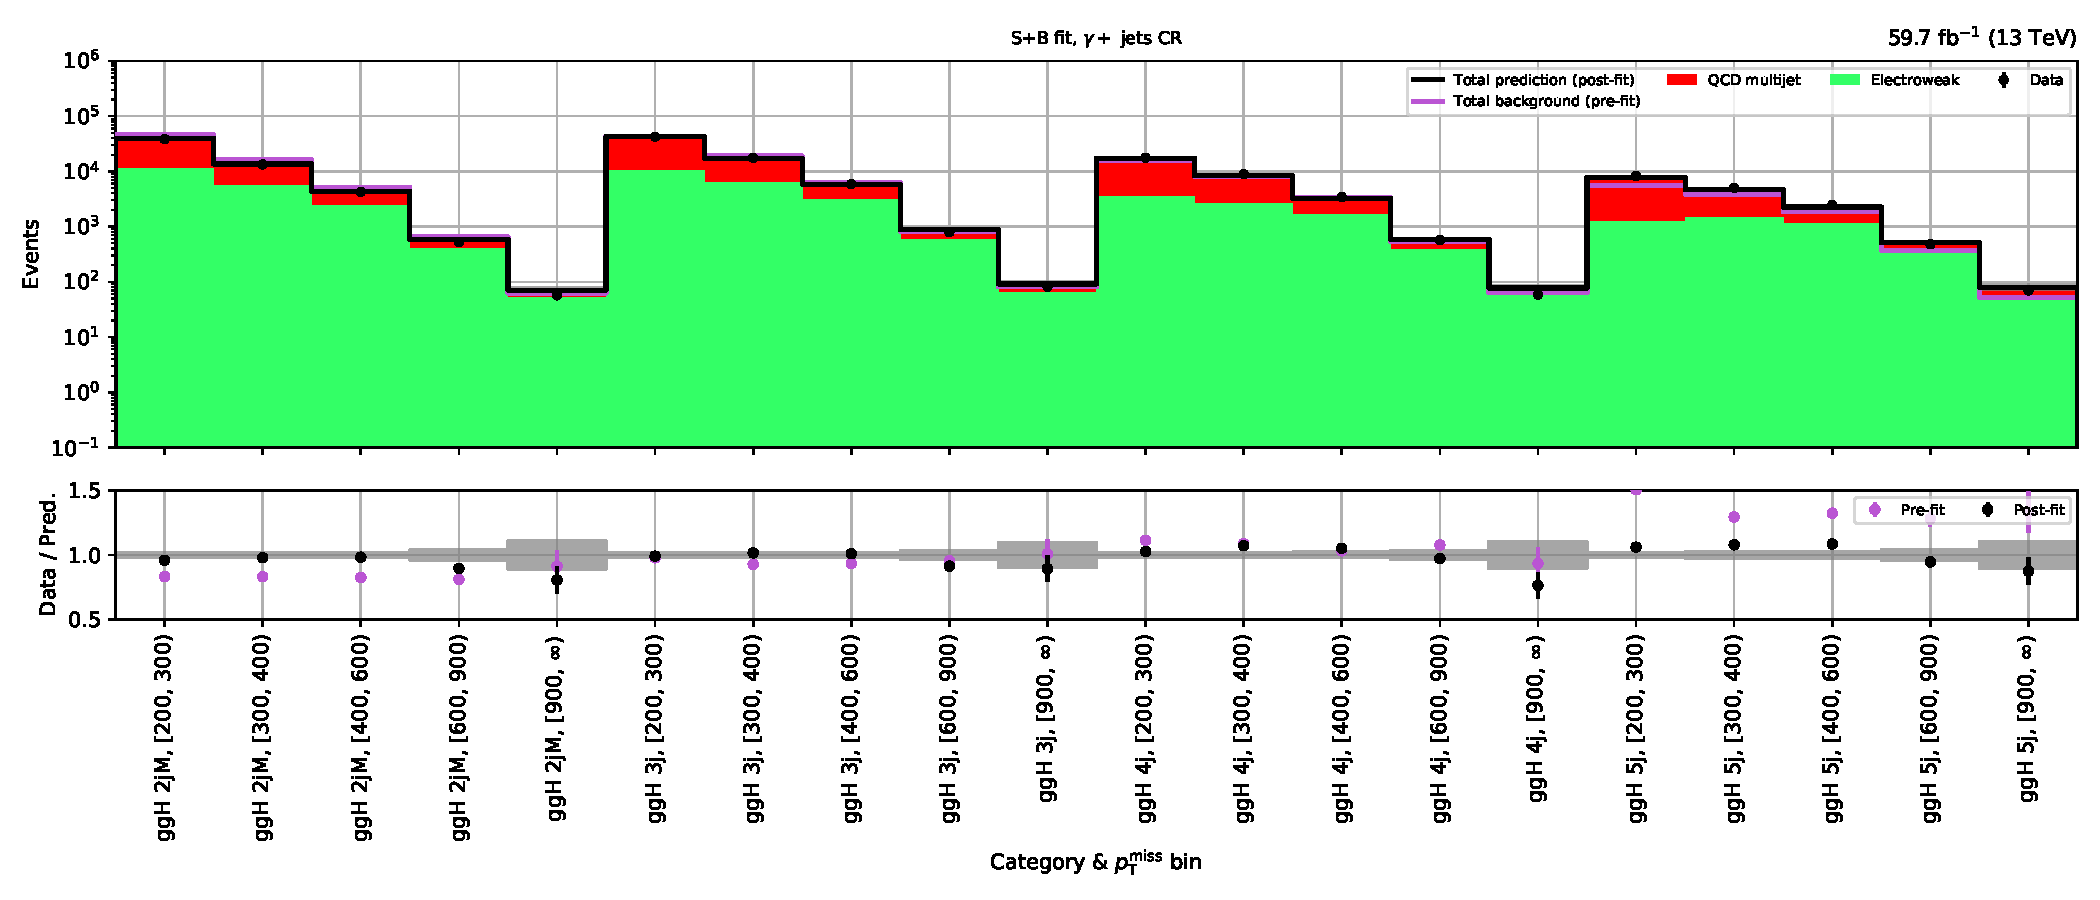
\includegraphics[width=\textwidth]{chapters/higgstoinv/figures/mountain_ranges/2018/ggF/Photon_tree_fit_s-abs_values_ggF_cats.pdf}
        \caption{\ggH --- \singlePhotonCr \gls{CR} (2018)}
    \end{subfigure}
    \caption[Post-fit yields for each \ggH subcategory and \ptmiss bin in the lepton and photon control regions for the 2018 dataset]{Post-fit yields for each \ggH subcategory and \ptmiss bin in the lepton and photon \glspl{CR} for the 2018 dataset. The total background pre-fit and post-fit is compared in the lower panel of each subfigure.}
    \label{fig:htoinv_mountain_range_ggF_2018_CRs}
\end{figure}
